\documentclass[a4paper, 11pt, bibliography=totoc, abstract=true]{scrreprt}  
\usepackage[utf8]{inputenc}
\usepackage[english,ngerman]{babel}
\usepackage{graphicx}
\graphicspath{ {./images/} }
\usepackage{setspace}
\usepackage{lipsum}
\usepackage{geometry}
\usepackage{dirtree}
\usepackage{xurl}
\usepackage[breaklinks]{hyperref}
\usepackage{cleveref}
\usepackage{caption}
\usepackage{subcaption}
\usepackage{adjustbox}

%Abbildungen formatieren
\usepackage{float}

\renewcommand{\sectfont}{\rmfamily\bfseries}
%\usepackage{subfigure}\hyphenation{Bit-rate}

%Einrücken nach Absatz verhindern
\setlength{\parindent}{0pt}

%%%%%%%%%%%%%%%%%%%%%%%%%%%%%%%%%%%
%Seiten Kopf- und Fußzeilen
\usepackage[automark,						
		headsepline,								
		plainfootsepline, 
		]{scrlayer-scrpage}

\automark[section]{chapter} 
\pagestyle{scrheadings}			

\clearscrheadings	% Alte Kopfformatierungen entfernen
\clearscrplain		% Alte Plain-Formatierung entfernen
\clearscrheadfoot   % Alte Fußzeile entfernen
\cfoot[\pagemark]{\pagemark} % Seitenzahl zentriert in Fußzeile 
\ihead{\leftmark}
\ohead{\rightmark} 
 
%%%%%%%%%%%%%%%%%%%%%%%%%%%%%%%%%%%


\usepackage{array}
\usepackage{footnote}
\usepackage{listings}
\usepackage{tikz}
\usepackage{./tikz-uml}
\usepackage{pgf-umlsd}
\usepgflibrary{arrows} % for pgf-umlsd

\usetikzlibrary{shapes,arrows, positioning}
\usepackage{xcolor}

%BIB
\usepackage{cite}
\bibliographystyle{eg-alpha}

\renewcommand{\lstlistingname}{Codeausschnitt}
\definecolor{darkgreen}{rgb}{0.0, 0.5, 0.0}

\lstdefinelanguage{JavaScript}{
  keywords={typeof, new, true, false, catch, function, return, null, catch, switch, var, if, in, while, do, else, case, break},
  keywordstyle=\color{blue}\bfseries,
  ndkeywords={class, export, boolean, throw, implements, import, this},
  ndkeywordstyle=\color{darkgray}\bfseries,
  identifierstyle=\color{black},
  sensitive=false,
  comment=[l]{//},
  morecomment=[s]{/*}{*/},
  commentstyle=\color{darkgreen}\ttfamily,
  stringstyle=\color{red}\ttfamily,
  morestring=[b]',
  morestring=[b]",
}

\lstdefinestyle{codeStyle}{
  language=Javascript, 
   extendedchars=true,
   basicstyle=\footnotesize\ttfamily,
  numbers=left,
   numberstyle=\footnotesize,
  stepnumber=1,
   numbersep=9pt,
  showspaces=false,
  showstringspaces=false,
  showtabs=false,
  tabsize=2,
  breaklines=true,
  breakatwhitespace=true,
  frame=single,
  rulecolor=\color{gray},
  captionpos=b,
  escapeinside={\%*}{*)},
}






%\geometry{a4paper, left=25mm, right=25mm, top=30mm, bottom=30mm}


\title{Webbasierte Multiplayer Schach-App}
\author{Jasper Paul Fülle}
\date{24. Mai 2023}

\begin{document}

\begin{titlepage}
\begin{center}
{\huge \textbf{Philipps-Universität Marburg}}\\[0.5cm]
\textbf{Fachbereich 12 - Mathematik und Informatik}\\[0.5cm]

\begin{figure}[h]
	\centering
		
\includegraphics[width=0.8\textwidth]{unilogo.pdf}
\end{figure}

{\huge \textbf{{\large \\[1cm]Bachelorarbeit}}}
\\[1cm]

{\Huge \textbf{Webbasierte Multiplayer\\ Schach-App}}
\\[1cm]

{\large von}\\
{\large Jasper Paul Fülle}\\
{\large Mai 2023}\\[3cm]

{\large
Betreuer:\\ Prof. Dr. Thorsten Thormählen\\[1cm]
Arbeitsgruppe Grafik und Multimedia Programmierung}

\end{center}
\end{titlepage}
\newpage
\thispagestyle{empty}
\section*{}
\newpage
\thispagestyle{empty}
\vspace*{7cm}
\textbf{\Large {Erklärung}}\\[0.5cm]
Ich, Jasper Paul Fülle (Wirtschaftsinformatikstudent an der Philipps-Universität Marburg, Matrikelnummer
3367654), versichere an Eides statt, dass ich die vorliegende Bachelorarbeit selbstständig verfasst und keine anderen
als die angegebenen Quellen und Hilfsmittel verwendet habe. Die hier vorliegende Bachelorarbeit wurde weder in ihrer jetzigen noch in einer ähnlichen Form einer Prüfungskommission vorgelegt.\\[1cm]
Marburg, 24. Mai 2023\\[0.5cm]
Jasper Fülle
\newpage
\shipout\null

%\setstretch {1.15}%Zeilenabstand setzen
\renewcommand{\abstractname}{Kurzzusammenfassung}

\newpage
\newpage\thispagestyle{empty}\hspace{1em}\newpage

\begin{abstract}
%Viele der in der Computergrafik verwendeten 3D-Modelle werden mit Hilfe von Dreiecksnetzen repräsentiert. ... (max. 1 Seite)

Das Interesse an Schach hat in den letzten Jahren immer mehr zugenommen und Online-Schachplattformen verzeichnen aktuell Rekorde an Benutzern und täglichen Spielen. Dies bietet die attraktive Möglichkeit eine Schach-App zu entwerfen und zu implementieren, deren Konzept Elemente aufgreift,

 welche bei bisherigen Schachplattformen kritisiert werden (kann ich eigentlich nicht schreiben, weil das nur meine Meinung ist ;()

welche mehr Anreize schaffen Partien zu spielen und soziale Interaktionen mit Fremden aber auch innerhalb einer Freundesgruppe zu fördern. 

Diese Bachelorarbeit hat das Ziel eine Webbasierte Multiplayer Schach-App zu entwerfen, die die Basis für Erweiterungen bildet, um konkurrenzfähig gegenüber den bisherigen Schachplattformen zu sein. Der Fokus liegt dabei besonders auf soziale Interaktionen, eine ansprechende Benutzererfahrung und Sicherheit hinsichtlich Benutzerdaten.
\end{abstract}
 
\newpage\thispagestyle{empty}\hspace{1em}\newpage

\begin{otherlanguage}{english}
\begin{abstract}
text text text text text text
text text text text
text text text text text text text text text text
(exakte englische Übersetzung der deutschen Kurzzusammenfassung)
\end{abstract}
\end{otherlanguage} 


\pagenumbering{Roman}
\setcounter{page}{1}
\tableofcontents
\newpage
\pagenumbering{arabic}
\setcounter{page}{1}

\chapter{Einleitung}
    \section{Motivation}
    Schach ist ein traditionsreiches und abwechslungsreiches Brettspiel, dessen Ursprung nicht genau bestimmt werden kann. Allerdings wird vermutet, dass das erste schachähnliche Spiel  \textit{Tschaturanga} seinen Ursprung in Nordindien um 600 n. Chr. hatte \cite{schachgeschichte}. Bis heute bleibt Schach ein beliebtes Spiel, das 2020 durch die Netflix Serie \textit{Damengambit} und 2022 durch den Betrugsvorwurf von Magnus Carlsen an seinen 19-jährigen Gegner Hans Niemann\footnote{Quelle: \url{https://www.sportschau.de/schach/magnus-carlsen-hans-niemann-ermittlungen-100.html} am 22. April 2023} eine größere Aufmerksamkeit erhielt (siehe Abbildung \ref{fig:Schachinteresse}). 
    
    \begin{figure}[ht]
\raggedleft
  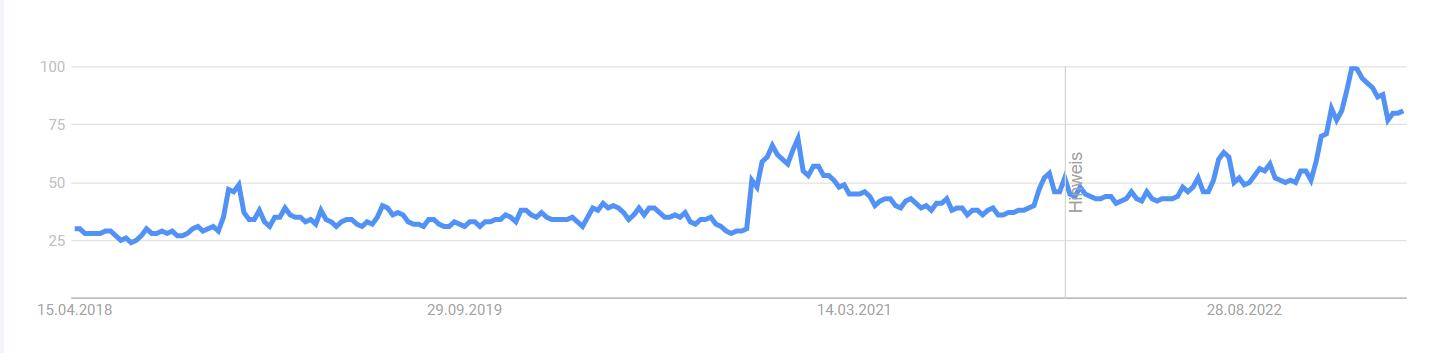
\includegraphics[width=\textwidth]{Schachentwicklung.jpg}
    \footnotesize\sffamily\textbf{Quelle:} \url{https://trends.google.de/}
  \caption{Relatives Suchinteresse des Wortes \textit{Chess} auf Google in den letzten 5 Jahren.}
  \label{fig:Schachinteresse}
\end{figure}

     Darüber hinaus hat Schach im digitalen Zeitalter eine neue Popularität erreicht. Online-Schachplattformen wie \url{chess.com} verzeichnen über zehn Millionen Schachpartien täglich\footnote{Quelle: \url{https://www.chess.com/about} am 12. Mai 2023}, während Schach Live-Streams auf Plattformen wie \url{twitch.com} Millionen von Followern anziehen\footnote{Quelle: \url{https://www.twitch.tv/chess} am 27. April 2023}.
     
Die Entwicklung einer webbasierten Multiplayer-Schach-App bietet eine einzigartige Gelegenheit, ein traditionsreiches und beliebtes Spiel im digitalen Zeitalter weiterzuentwickeln. Mein Ziel für diese Arbeit besteht darin, eine App zu entwickeln, die die Grundlagen einer Schach-App enthält und gleichzeitig eine solide Basis für zukünftige Erweiterungen und Verbesserungen bietet.
Insbesondere die Aussicht in Zukunft, innovative Funktionen zu integrieren, die bislang in den gängigen Schach-Apps nicht oder nicht kostenfrei vorhanden sind motiviert diese Arbeit. Durch die Entwicklung einer Schach-App mit neuen Funktionalitäten kann ich dazu beitragen, die Popularität von Schach zu steigern und vor allem das Spiel einem breiteren Publikum zugänglich zu machen.
    \section{Zielsetzung}
    Diese Bachelorarbeit hat das Ziel eine Schach-App zu entwerfen und zu implementieren, die eine intuitive User Experience und ein ansprechendes User Interface mit vielen nützlichen Funktionen beinhaltet. Bei der Anwendung soll dabei vor allem soziale Interaktionen im Zusammenhang mit Schach im Vordergrund stehen.
    
User Experience (kurz UX) bezieht sich darauf, wie ein Nutzer sich auf einer Anwendung bewegt und wie einfach und angenehm es für den Nutzer ist, die Funktionen der Anwendung zu verwenden.
    
    Unter User Interface (kurz UI) versteht man die visuelle und interaktive Gestaltung von Benutzeroberflächen. Es umfasst die Gestaltung von Buttons, Formularen und anderen visuellen Komponenten, sowie das Feedback dieser Komponenten, wie zum Beispiel die Rückmeldung einer fehlgeschlagenen Anmeldung.
    Zusammengefasst beschäftigt sich UX damit, wie man eine Anwendung verwendet und UI damit, wie die Benutzeroberfläche der Anwendung aussieht.\cite{webdesign}
        
        Funktionen der Schach-App sind unter anderem das Registrieren und Anmelden, das Versenden, Annehmen und Ablehnen von Freundschaftsanfragen, das Zuschauen bei laufenden Spielen, das Herausfordern von Freunden zu Schachspielen und natürlich das Spielen von Schachpartien mit einem Chat und verschiedenen Einstellungsmöglichkeiten der Spielzeiten selbst.
    Dabei wird besonderer Wert auf die Verwendung moderner Web-Technologien wie React, Node.js, Socket.IO, Redis und PostgeSQL gelegt, um eine optimale Benutzererfahrung und Skalierbarkeit zu gewährleisten. Darüber hinaus soll die Arbeit einen Überblick über die technischen Herausforderungen und Lösungen im Zusammenhang mit der Implementierung einer solchen Schach-App bieten.
    
Die Anwendung dient hauptsächlich als Basis Schach-App für Erweiterungen. So ist das Webdesign noch nicht responsiv, da mit neuen Erweiterungen die UI und UX ohnehin angepasst werden müsste, um weitere Funktionen zur Verfügung zu stellen.
    
    \section{Aufbau der Arbeit}
Diese Bachelorarbeit gliedert sich in sechs Hauptkapitel, die jeweils unterschiedliche Aspekte der Entwicklung und Implementierung der Schach-App behandeln.

Im ersten Kapitel, der \textit{Einleitung}, werden die Motivation für die Entwicklung der Schach-App, die Zielsetzung der Arbeit und der Aufbau der Arbeit selbst vorgestellt.

Das zweite Kapitel, \textit{Theoretische Grundlagen}, erläutert die Grundlagen von Schach als Spiel sowie die verwendeten Web-Technologien wie Node.js, Express, Socket.io, React und PostgreSQL, die für das Verständnis der nachfolgenden Kapitel wichtig sind.

Im dritten Kapitel, \textit{Systemarchitektur}, wird die Gesamtarchitektur der Schach-App beschrieben, einschließlich der Unterteilung in Frontend und Backend, der Datenbankstruktur und der Kommunikation zwischen den verschiedenen Komponenten.

Das vierte Kapitel, \textit{Implementierung}, geht auf die praktische Umsetzung der Schach-App ein, indem es die Entwicklungsprozesse für das Frontend und das Backend sowie die Integration der Datenbanken erläutert.

Das fünfte Kapitel, \textit{Tests und Evaluation}, behandelt die verschiedenen Tests, die durchgeführt wurden, um die Funktionalität, Usability, Performance und Sicherheit der Schach-App zu bewerten.

Im abschließenden sechsten Kapitel, \textit{Fazit und Ausblick}, werden die Ergebnisse der Arbeit zusammengefasst, eventuelle Limitationen diskutiert und mögliche Erweiterungen und Weiterentwicklungen für die Schach-App vorgeschlagen.

Die Arbeit endet mit dem \textit{Anhang}, der zusätzliche Grafiken und die Liste der verwendeten Literatur enthält.

\section{Verwandte Arbeiten}
\label{sec:Verwandte Arbeiten}
Es gibt vor allem zwei große online Schachplattformen: \url{chess.com} und \url{lichess.org}.

Dabei war \url{chess.com} auf Platz 114 und \url{lichess.org} auf Platz 209 der Webseiten mit am meisten Web-Traffic weltweit im April 2023\footnote{Quelle: \url{https://www.similarweb.com/website/chess.com/vs/lichess.org/\#overview} am 12. Mai 2023}.

\subsection{Chess.com}
Chess.com zeichnet sich durch vielfältige Funktionen, einer verspielten UI und sehr vielen Benutzern aus. Was im Vergleich zu Lichess jedoch schnell bemerkbar ist, ist die Kommerzialisierung.

Chess.com hat auf seiner gesamten Seite viel Werbung und bietet viele Funktionen nur bei einem monatlichen Abonnement gegen Geld an (siehe Abbildung \ref{fig:chess.com-abo}). Zu diesen Funktionen gehören Analysen der Schachpartien, mehrere Spiele gleichzeitig zu spielen, der Zugriff auf Lektionen zum lernen von Schach und vieles weitere.

  \begin{figure}[htb]
  \centering
  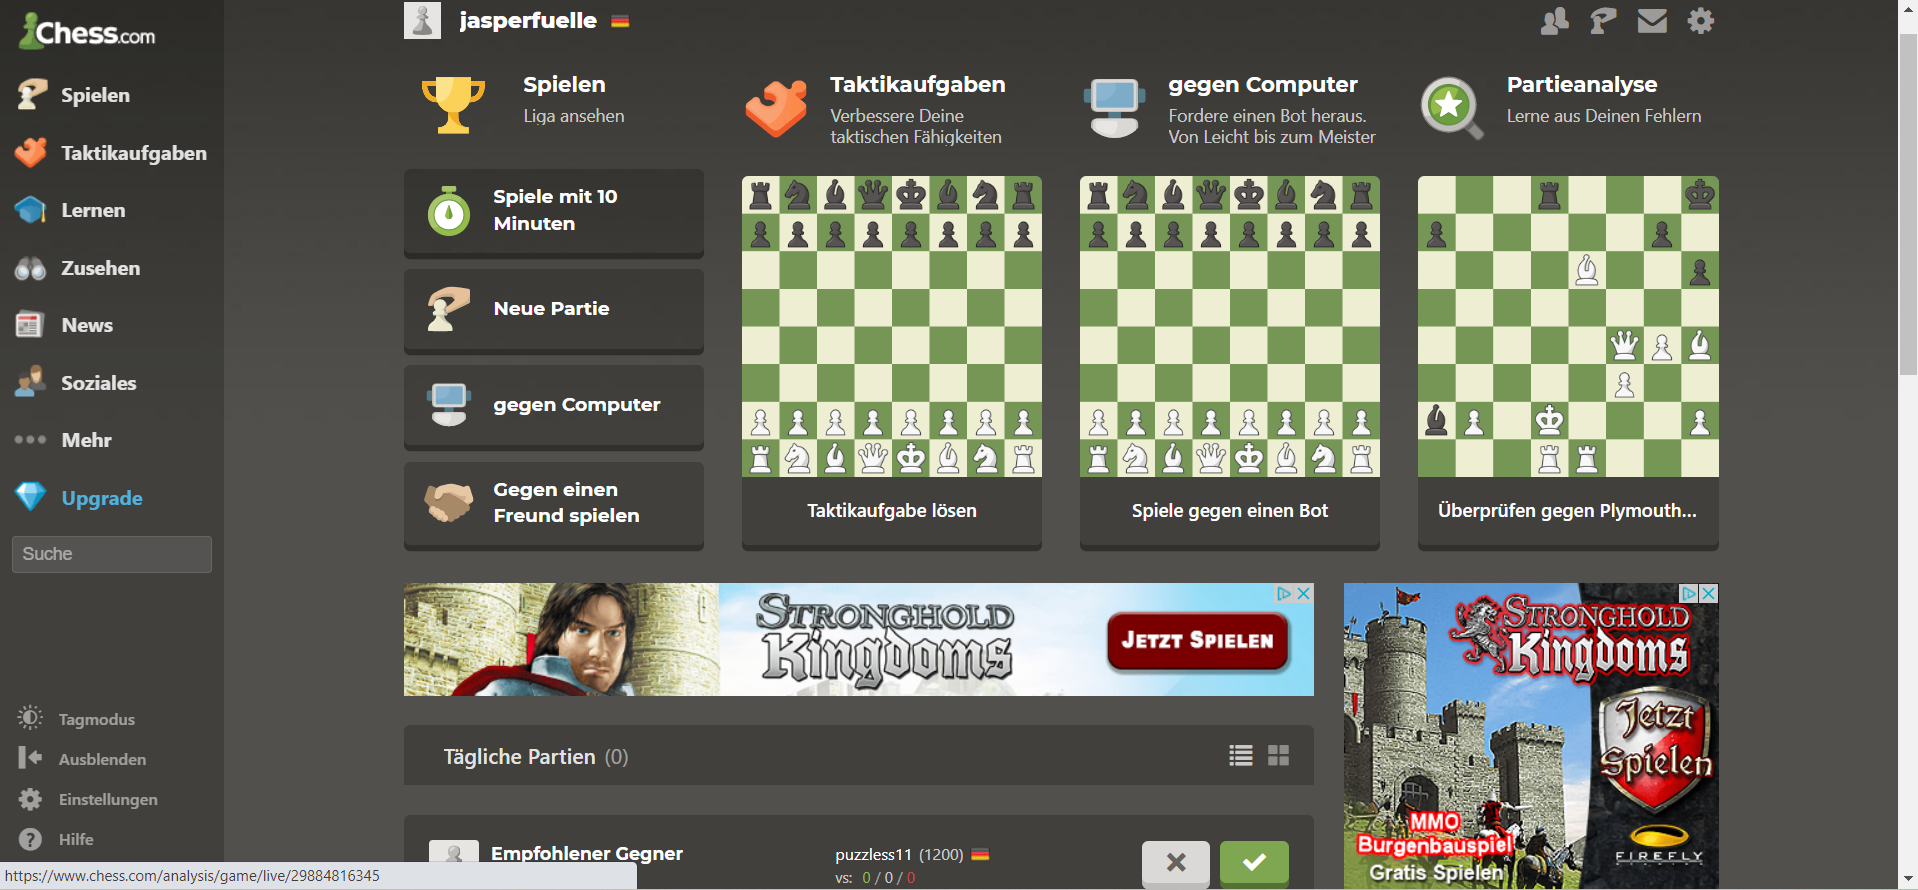
\includegraphics[width=\textwidth]{chess.com.png}
\raggedleft
    \footnotesize\sffamily\textbf{Quelle:} \url{https://www.chess.com/home} am 12. Mai 2023
  \caption{Home-Bildschirm von Chess.com}
  \label{fig:chess.com}
\end{figure}

  \begin{figure}[htb]
  \centering
  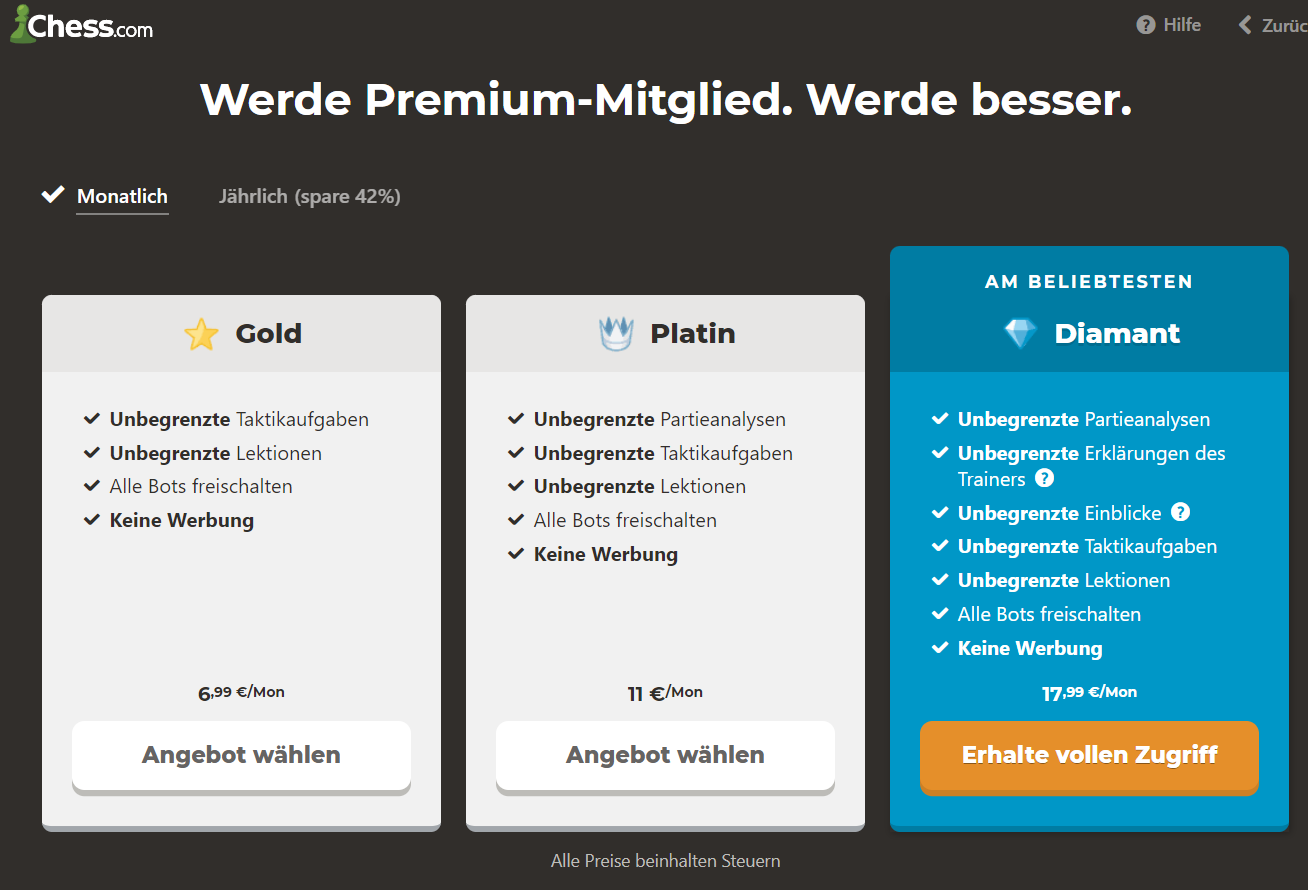
\includegraphics[width=0.7\textwidth]{Abo-chess.com.png}
  
\raggedleft

    \footnotesize\sffamily\textbf{Quelle:} \url{https://www.chess.com/membership?c=navbar} am 12. Mai 2023
  \caption{Abonnement Möglichkeiten von Chess.com}
  \label{fig:chess.com-abo}
\end{figure}

Die Funktionen die Chess.com zur Verfügung stellt (kostenpflichtige, als auch kostenfreie) sind dafür sehr umfangreich. Es gibt Clubs mit Turnieren, es gibt verschiedene Spielmodi, die beispielsweise ermöglichen zu viert ein Schachspiel zu spielen und Taktikaufgaben zum lösen.

Chess.com zeichnet sich auch durch seine Online-Präsenz auf Plattformen wie YouTube\footnote{Quelle: \url{https://www.youtube.com/@chess} am 12. Mai 2023} oder twitch\footnote{Quelle: \url{https://www.twitch.tv/chess} am 12. Mai 2023} aus.


\subsection{Lichess}
Lichess wirbt vor allem damit, dass es komplett kostenfrei verwendbar ist, keine Werbung hat und keine Registrierung nötig ist um zu spielen. Auch Funktionen wie Analysen eines Spiels sind für alle Benutzer uneingeschränkt verfügbar. Die Finanzierung von \url{lichess.org} basiert auf Spenden und die Entwicklung übernehmen Freiwillige\footnote{Quelle: \url{https://lichess.org/about} am 12. Mai 2023}. Der gesamte Code ist Open-Source und für jeden einsehbar.

Lichess ist dunkel und modern gehalten. Einige Funktionen sind auf dem Desktop schwer zugänglich, während sie auf einem Mobil-Gerät in der App gar nicht verfügbar sind. Dazu zählen auch soziale Interaktionen wie Gruppen. Sie sind wenig ausgebaut und schwierig, bis gar nicht, auffindbar.

  \begin{figure}[htb]
  \centering
  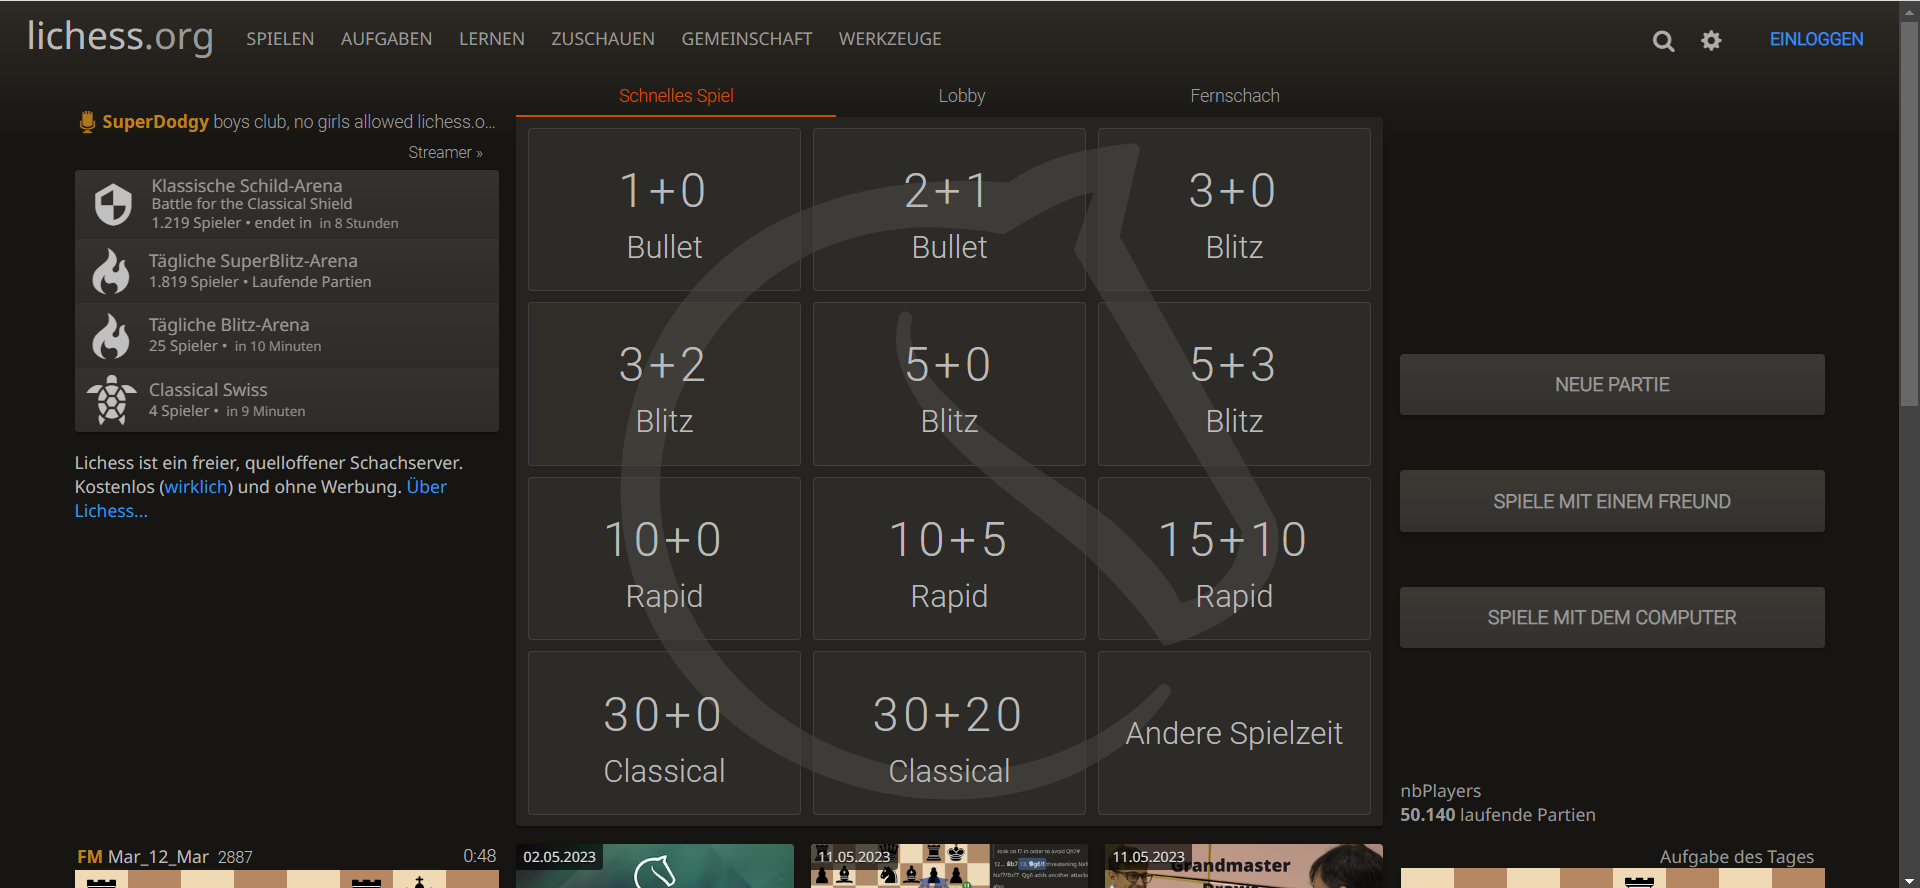
\includegraphics[width=\textwidth]{lichess.png}
\raggedleft
    \footnotesize\sffamily\textbf{Quelle:} \url{lichess.org} am 12. Mai 2023
  \caption{Der Lichess Desktop Home-Bildschirm}
  \label{fig:lichess}
\end{figure}
\newpage
\newpage\thispagestyle{empty}\hspace{1em}\newpage
	\chapter{Theoretische Grundlagen}
    \section{Schach}
    \label{sec:schach-theorie}
   Schach ist ein strategisches Brettspiel für zwei Spieler, welches auf einem quadratischen Spielfeld mit 64 Feldern gespielt wird. Jeder Spieler beginnt mit 16 Figuren und das Ziel des Spiels ist es, den König des Gegners schachmatt zu setzen, indem man ihn bedroht, ohne dass der Gegner den Angriff verhindern kann. 
   
   Wie Figuren sich bewegen und andere Figuren schlagen erkläre ich nicht explizit, lediglich zwei Sonderregeln des Schachs und Schachuhren werde ich genauer erklären, da diese bei der Umsetzung des Spiels gesondert gehandhabt werden müssen.
   
   Die erste ist die so genannte \textit{en passant}-Regel. Dabei ist es einem Bauern möglich einen gegnerischen Bauer diagonal zu schlagen, falls dieser zwei Felder gezogen ist und nun auf der gleichen Höhe wie der eigene Bauer steht (siehe Abbildung \ref{fig:en-passant}).
   
   Die zweite Zusatzregel ist die \textit{Bauernumwandlung}. Sie besagt, dass falls ein Bauer die gegnerische Grundreihe erreicht, dieser Bauer in eine Dame, einen Springer, einen Turm oder einen Läufer umgewandelt werden kann (siehe Abbildung \ref{fig:promotion}).
   
     \begin{figure}[ht]
\raggedleft
  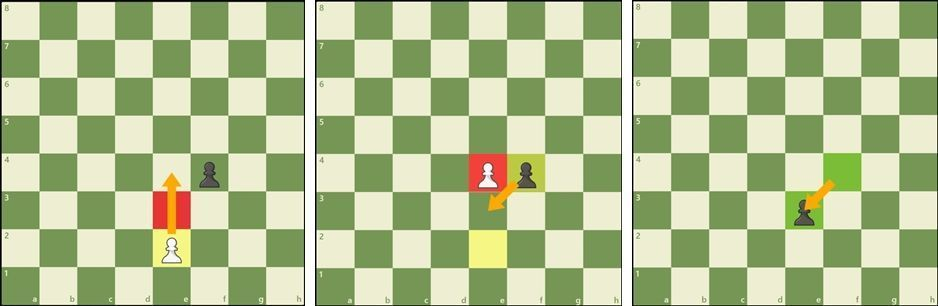
\includegraphics[width=\textwidth]{en-passant.jpeg}
    \footnotesize\sffamily\textbf{Quelle:} \url{https://www.chess.com/de/schachregeln}
  \caption{Die Zusatzregel \textit{en passant}}
  \label{fig:en-passant}
\end{figure}

  \begin{figure}[ht]
\centering
  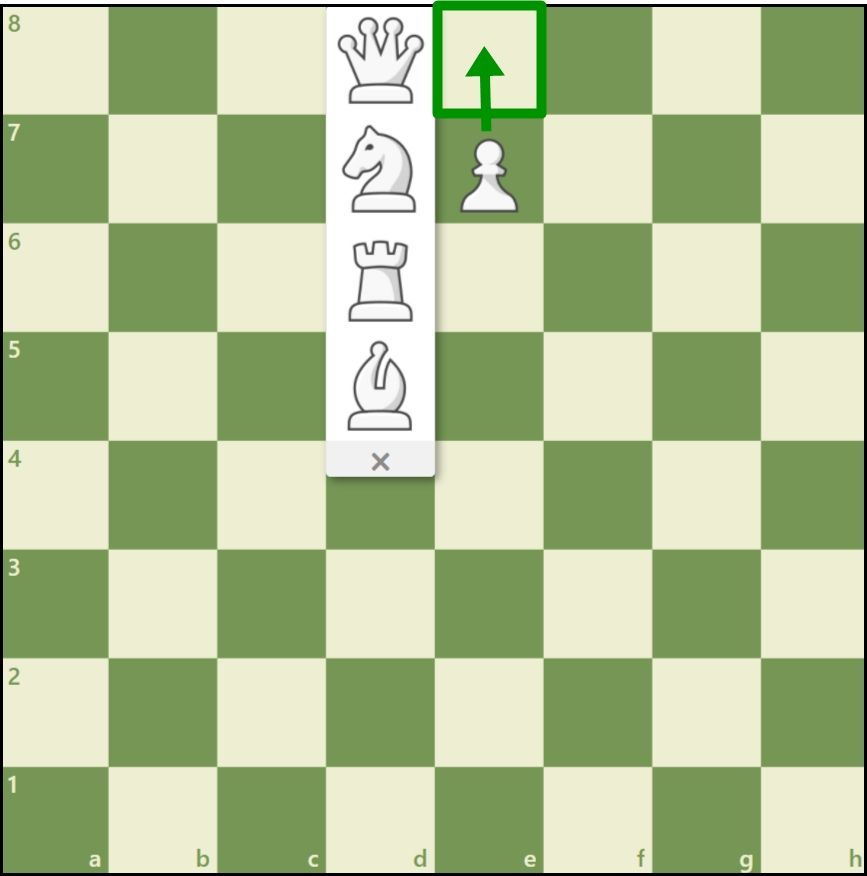
\includegraphics[height=0.4\textwidth]{promotion.jpeg}
   
   
\raggedleft
    \footnotesize\sffamily\textbf{Quelle:} \url{https://www.chess.com/de/schachregeln}
  \caption{Die Zusatzregel \textit{Bauernumwandlung}}
  \label{fig:promotion}
\end{figure}

Die Notation von Schachuhren besteht aus zwei Zahlen, die mit einem Plus getrennt werden, wie zum Beispiel \glqq 10 + 5\grqq .  Hier steht die erste Zahl, in diesem Fall 10, für die Gesamtzeit, die jedem Spieler zur Verfügung steht, also 10 Minuten. Die zweite Zahl, hier 5, wird als Inkrement bezeichnet. Dies bedeutet, dass nach jedem Zug eines Spielers diesem Spieler zusätzlich 5 Sekunden hinzugefügt werden. Dadurch haben Partien mit Inkrement mehr Zeit, je mehr Züge gespielt werden.

Bei Online-Schachpartien ist es zusätzlich üblich, eine bestimmte Startzeit für den ersten Zug jedes Spielers verstreichen zu lassen. Dies gewährleistet, dass die Uhren erst zu laufen beginnen, wenn beide Spieler bereit sind und mitbekommen haben, dass das Spiel gestartet wurde.

    \section{Web-Technologien}
        \subsection{Node.js und Express}
        \subsubsection{Node.js und seine Vorteile}
        \label{sec:node.js}
Node.js ist eine JavaScript-Laufzeitumgebung, welche erstmals 2009 angekündigt wurde\footnote{Quelle: \url{https://www.youtube.com/watch?v=EeYvFl7li9E} am 22. April 2023} und speziell für die Entwicklung von skalierbaren Netzwerkanwendungen entworfen wurde \cite{nodejs}. Skalierbarkeit bedeutet, dass mit steigender Benutzeranzahl der Ressourcenverbrauch idealerweise linear steigt. Zu den relevanten Ressourcen von Webanwendungen gehören Rechenleistung, Ein-/Ausgabeoperationen (kurz I/O) und Arbeitsspeicher, wobei Node.js vor allem die Skalierbarkeit von I/O intensiven Anwendungen verbessert \cite{nodejsbook}.
I/O-Zugriffe sind beispielsweise Zugriffe auf Datenbanken, Webservices oder auf das Dateisystem. Node.js setzt dabei vollständig auf asynchrone Zugriffe. Dabei wartet der Thread nicht auf das Ergebnis eines I/O-Zugriffs, sondern führt andere Aufgaben aus, bis das Ergebnis verfügbar ist. Anschließend wird eine zuvor definierte Callback Funktion (siehe Codeausschnitt \ref{lst:callback}) durchgeführt. Bei einem synchronen Zugriff, wie es bei einigen anderen Laufzeitumgebungen der Fall ist, würde der Thread auf das Ergebnis warten und dieses anschließend weiterverarbeiten, wobei jedoch sein Speicherplatz zum Teil belegt bleibt.\cite{nodejsbook} Die Vorteile hinsichtlich der Skalierbarkeit werden jedoch erst bei einer hohen Anzahl von Zugriffen erkennbar.

\begin{lstlisting}[style=codeStyle, caption={Beispiel einer Callback Funktion \textbf{Quelle: } \cite{nodejsbook}}, label={lst:callback}]
database.query(  "SELECT * FROM user",  function(result) {
result...
});
\end{lstlisting}


Ein weiterer Vorteil der Nutzung von Node.js ist die Nutzung der gleichen Programmiersprache für Frontend und Backend.
In einem Team-Projekt kann das besonders hilfreich sein, da Kommunikationsbarrieren durch unterschiedliche Programmiersprachen von Frontend und Backend niedriger sind. Natürlich versteht deshalb der Frontend-Entwickler nicht alles was  der Backend-Entwickler macht und umgekehrt, jedoch gibt es eine gemeinsame Grundlage. Neben den Kommunikationsvorteilen ermöglicht die Verwendung von der gleichen Programmiersprache im Frontend und Backend das Teilen von Code. So ist es zum Beispiel möglich Callback Funktionen vom Frontend an das Backend zu senden und dort aufzurufen.

Node.js basiert auf der Verarbeitung von Requests vom Frontend und dem zurück senden von einem Result mittels dem HTTP-Protokoll. Das HTTP-Protokoll verwendet verschiedene Methoden wie GET, POST, PUT und DELETE, um unterschiedliche Aktionen durchzuführen  \cite{expressbook}. Zum Beispiel wird GET zum Abrufen von Informationen verwendet, während POST zum Senden von Daten verwendet wird. Die Art und Weise wie ein Request verarbeitet werden soll ist dabei selbst zu definieren (siehe Abbildung \ref{fig:node-request}). Dabei kann der Request sein, eine bestimmte Seite zu laden, womit dann mit der entsprechenden HTML-Datei geantwortet wird, oder es kann als API genutzt werden, um Beispielsweise Daten einer Datenbank zu übermitteln. Um die Verarbeitung dieser Anfragen weniger komplex zu gestalten gibt es die Erweiterung \textit{Express} für Node.js.

  

  \begin{figure}[ht]
  \centering
  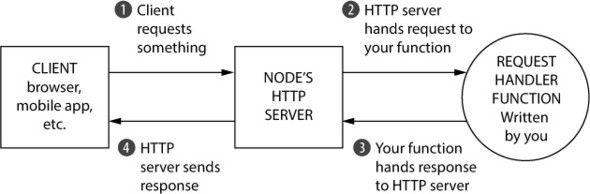
\includegraphics[width=\textwidth]{node-request.jpg}
\raggedleft
    \footnotesize\sffamily\textbf{Quelle:} \cite{expressbook}
  \caption{Ablauf einer Anfrage an einen Node.js Server}
  \label{fig:node-request}
\end{figure}


\subsubsection{Express}
\label{sec:express}
\textit{Express} ist ein leichtgewichtiges und sehr beliebtes Web-Frameworks, welches unter Node.js zur Verfügung steht. Es dient zur Vereinfachung der API von Node.js und stellt hilfreiche Funktionen bereit \cite{expressbook}. Es ermöglicht beispielsweise die Verwendung von \textit{Middleware} und \textit{Routing}.

\textit{Middleware} ermöglicht, dass eine Anfrage an den Node.js Server nicht ausschließlich von einer Funktion bearbeitet werden muss, welche das Ergebnis zurücksendet, sondern von mehreren Funktionen, die sich um verschiedene Teile der Request kümmern (siehe Abbildung \ref{fig:express-request}). Diese Funktionen heißen \textit{Middleware}. Dabei gibt es eine von uns definierte Reihenfolge der Middlewares. Zum Beispiel können wir definieren, dass zu erst der Request von einer Middleware geloggt werden soll, anschließend soll der Benutzer authentifiziert werden und falls der Benutzer eine URL aufrufen möchte, für die er keine Berechtigung hat wird eine \glqq not authorized\grqq{ }Seite zurück gesendet und die nächste Middleware wird nicht aufgerufen. Ansonsten wird die nächste Middleware der Kette ausgeführt, wie zum Beispiel das senden von Informationen (siehe Abbildung \ref{fig:middleware-beispiel}). Ein Vorteil der Nutzung von Middlewares ist, dass es bereits viele vordefinierte Middlewares (auch von Dritten) gibt, welche nützliche Funktionalitäten mitbringen. Die Anfrage des Frontends in mehrere kleinere Funktionen aufzuteilen, anstatt eine Funktion zu schreiben, welche sich um all dies kümmert verringert die Komplexität und erhöht die Modularität.

  \begin{figure}[h]
  \centering
  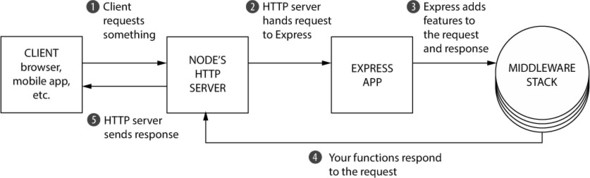
\includegraphics[width=\textwidth]{express-request.jpg}
\raggedleft
    \footnotesize\sffamily\textbf{Quelle:} \cite{expressbook}
  \caption{Ablauf einer Anfrage an einen Node.js Server mit Express}
  \label{fig:express-request}
\end{figure}



  \begin{figure}[h!]
  \centering
  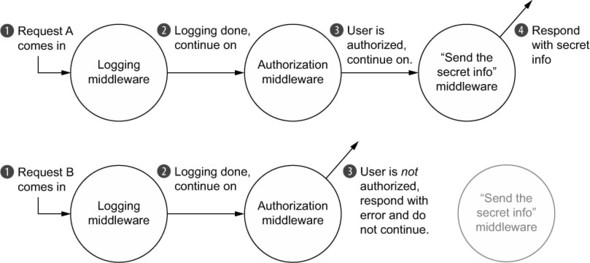
\includegraphics[width=0.7\textwidth]{Middleware-Beispiel.jpg}
  
  \vspace{10mm}
  
  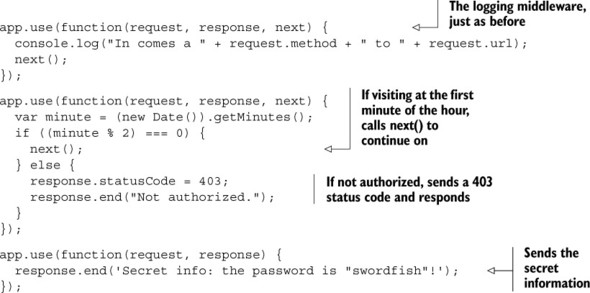
\includegraphics[width=0.7\textwidth]{Middleware-Beispiel-2.jpg}
  
\raggedleft
    \footnotesize\sffamily\textbf{Quelle:} \cite{expressbook}
  \caption{Beispiel der Nutzung von Middlewares}
  \label{fig:middleware-beispiel}
\end{figure}

\textit{Routing} hilft dabei zu identifizieren bei welchem Request welche Middleware ausgeführt werden soll (siehe Abbildung \ref{fig:routing-beispiel}). Beispielsweise kann eine Anfrage an die URL \url{/auth} mit den angegeben Anmeldedaten des Benutzers gesendet werden. Unter diesem Pfad können wir dann bestimmte Middlewares verwenden, welche sich mit der Authentifizierung des Benutzers befassen.

  \begin{figure}[ht]
  \centering
  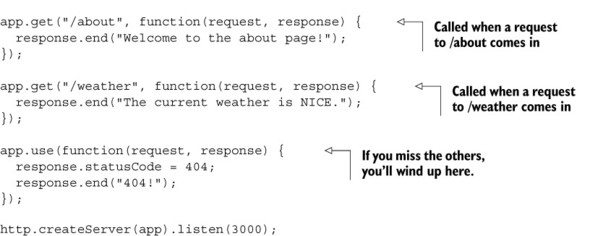
\includegraphics[width=\textwidth]{express-routing-example.jpg}
\raggedleft
    \footnotesize\sffamily\textbf{Quelle:} \cite{expressbook}
  \caption{Beispiel der Nutzung von Routing}
  \label{fig:routing-beispiel}
\end{figure}

        \subsection{Socket.io}
        \label{sec:socket.io}
Die Kommunikation mit dem HTTP-Protokoll über Express hat den Nachteil, dass für jeden Datenaustausch eine neue Verbindung aufgebaut und wieder geschlossen wird, was zu einer Latenz führt, welche für Echtzeit-Anwendungen ungeeignet ist. Diese Problematik behebt das Framework \textit{socket.io}. %QUELLE BENÖTIGT%

Es ermöglicht eine direkte, bidirektionale Echtzeitübertragung von Daten mittels Websockets, long-polling und fünf anderen Protokollen zwischen den Clients und dem Server. Diese Echtzeitkommunikation ist für viele Spiele, wie auch für diese Schach-App, essentiell. So können beim Spielen mit Schachuhr Millisekunden entscheidend sein.
Neben der Echtzeitkommunikation überprüft socket.io unter anderem Timeouts, Verbindungsabbrüche, stellt Verbindungen automatisch wieder her und sorgt dafür, dass die Events in der richtigen Reihenfolge beim Server und beim Client ankommen. 

Die Kommunikation mit Socket.io läuft ausschließlich über Events. So kann man sowohl beim Client, als auch bei dem Server Eventlistener definieren, die auf ein bestimmtes Event hören und darauf hin eine Funktion auf den übertragenen Daten anwenden. Diese Eventlistener (definiert mit der Funktion \verb|.on()|) haben als ersten Parameter den Namen des Events als String, auf den dieser Listener hören soll und als zweiten Parameter die auszuführende Callback Funktion, welche mit den Parametern aufgerufen wird, die beim senden des Events übertragen wurden.

Events können basierend auf verschiedenen Aktionen wie zum Beispiel dem Drücken eines Buttons im Frontend oder als Reaktion eines eingegangenen Events auf dem Server gesendet werden (mit der Funktion \verb|.emit()|) (siehe Abbildung \ref{fig:socket.io-beispiel}). Der erste Parameter der \verb|emit|-Funktion ist wieder der Name des Events als String und im Anschluss kann man beliebig viele Parameter übertragen mit denen die Callback-Funktion des Listeners aufgerufen wird.


  \begin{figure}[ht]
\raggedleft
  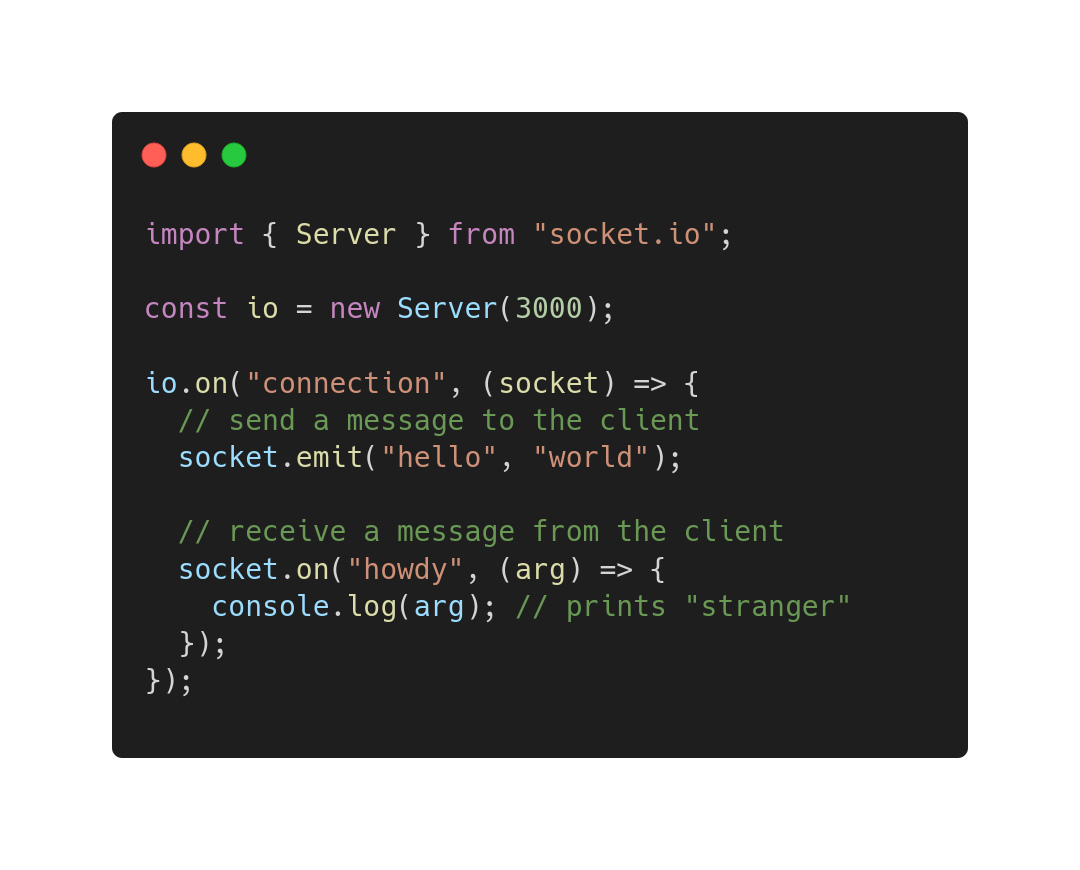
\includegraphics[width=0.45\textwidth]{socket.io-server-beispiel.png}
  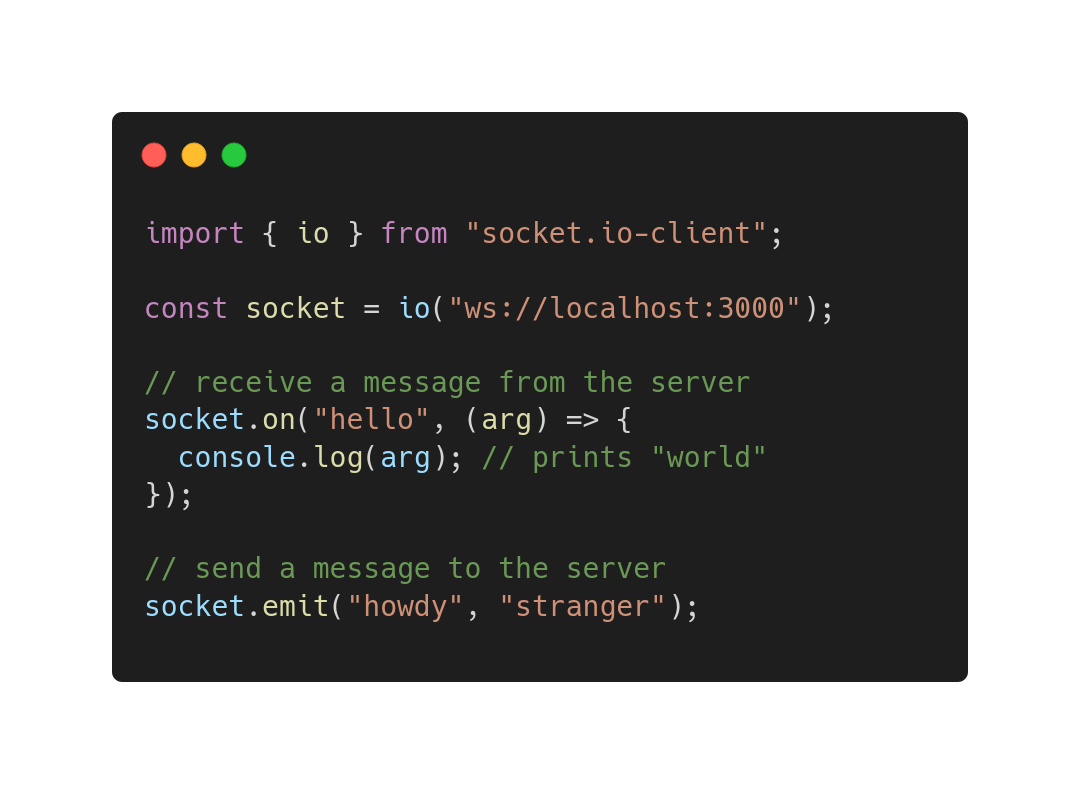
\includegraphics[width=0.45\textwidth]{socket.io-client-beispiel.png}
    \footnotesize\sffamily\textbf{Quelle:} \cite{socketio}
  \caption{Simples Beispiel der Initialisierung einer socket.io Verbindung und das Senden und Empfangen von Events}
  \label{fig:socket.io-beispiel}
\end{figure}

Ein wichtiges Feature von socket.io sind die Räume\footnote{Quelle: \url{https://socket.io/docs/v4/rooms/} am 22. April 2023}. Sockets im Backend können ihnen Beitreten und sie Verlassen. Serverseitig kann man dadurch an alle Sockets, die in einem bestimmten Raum sind etwas senden, ohne es allen einzeln schicken zu müssen (siehe Abbildung \ref{fig:socket.io-room}). Hier kann man sich entschließen das Event an alle clients im Raum zu versenden (\verb|io.to(...).emit(...)|) oder an alle, außer den sender (\verb|socket.to(...).emit(...)|) (siehe Codeausschnitt \ref{lst:socket-rooms}).


  \begin{figure}[ht]
  \centering
  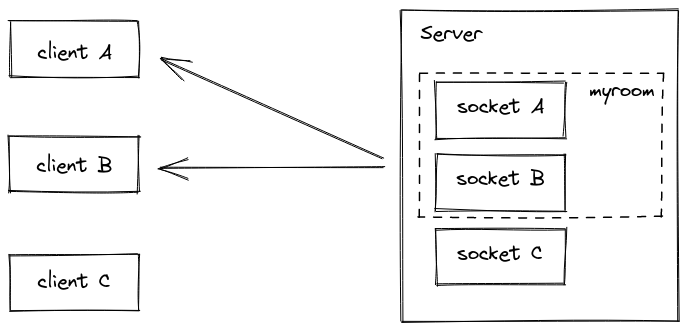
\includegraphics[width=\textwidth]{socket.io-rooms.png}
\raggedleft
    \footnotesize\sffamily\textbf{Quelle:} \url{https://socket.io/docs/v4/rooms/} am 27. April 2023
  \caption{Darstellung eines Raumes \textit{myroom} mit zwei sockets}
  \label{fig:socket.io-room}
\end{figure}

Des weiteren erhält jede socket beim Verbinden eine eigene ID, die ebenfalls als Raum genutzt werden kann. Dementsprechend ist \verb|io.to(socket.id).emit('hello');| äquivalent zu \verb|socket.emit('hello');|.

Socket.io unterstützt wie Express Middlewares, welche bei einem Verbindungsaufbau ausgeführt werden. Dabei sind die übergebene Argumente die socket und die next Funktion als nächste Middleware.
Es bietet sich daher an Authetifikation oder die Initialisierung von Listenern als Middleware  zu behandeln.


\begin{lstlisting}[style=codeStyle, caption={Beispiel zum Beitreten Raums und das senden eines Events in diesen Raum}, label={lst:socket-rooms}]
//Server
io.on("connection", (socket) => {
  socket.join("Chat");
  socket.on("message", (text) => {
  	socket.to("Chat").emit("message", text);
  }
  //Empfangen der Nachricht und weiterleiten an alle im Raum, ausser Sender.
});

//Frontend
...
socket.emit("message", "hello world"); //Senden
socket.on("message", text => console.log(text)); //Empfangen
...
\end{lstlisting}
//QUELLE socket.io im nodejsbook
        \subsection{React}
        \subsubsection{React}
        \label{sec:react}
React ist eine der beliebtesten (nach einer Umfrage von 2022 von Stack Overflow sogar die beliebteste \cite{stack-overflow-survey}) Frontend Javascript Bibliotheken. Es basiert auf Komponenten, welche wiederverwendbar und kombinierbar sind und vereinfacht die Verwaltung von Interaktionen mit User Interfaces. Dabei benutzt React eine Syntax Erweiterung namens \textit{JSX}. Mit dieser Erweiterung ist es erlaubt HTML Elemente in JavaScript Dateien zu verwenden, welches es ermöglicht die Logik hinter getrennten HTML und JavaScript Dateien in eine Datei zu kombinieren. Die Idee hinter React ist, dass wenn sich nur ein bestimmter Teil des User Interfaces im Vergleich zum aktuell sichtbaren User Interface ändert, auch nur dieser Teil neu gerendert wird und nicht das ganze User Interface. Diese reaktiven Änderungen veranlasst React mittels seiner \textit{Hooks} \cite{react-key-concepts}.

Ich werde die Art und Weise wie React und seine Hooks funktionieren an dem Beispiel \ref{lst:react-example} erklären.
In diesem Beispiel implementieren wir die Komponente \textit{ExampleComponent}, welche zum Beispiel mittels dem Tag \verb|<ExampleComponent initialCount={10} loadingDelay={3000} />| verwendet werden kann. 

Die zwei übergebenen Variablen \textit{initialCount} und \textit{loadingDelay} werden auch \textbf{props} genannt, welche in der Komponente verwendet werden können. Eine Komponente ist eine Funktion, welche als Rückgabe den HTML-Code hat, welcher angezeigt werden soll.

Die Komponente hat den lokalen State \textit{count}, welchen wir mittels der \textbf{useState} Hook initialisieren. Ein State beschreibt einen Zustand der Komponente und eine Änderung veranlasst die Komponente neu zu laden. Die Funktion \textit{useState} nimmt als Argument den initialen Wert des States und gibt uns zwei Elemente zurück, einmal der sich verändernde State \textit{count} und die Funktion \textit{setCount}, um einen neuen Wert in den State \textit{count} zu schreiben. Der zurückgegebenen Funktion \textit{setCount} kann entweder ein konkreter Wert übergeben werden, oder aber eine Funktion welche beschreibt wie der neue Wert sich aus dem alten Wert bilden soll (siehe Zeile 31 in Beispiel \ref{lst:react-example}).

Die Hook \textbf{useEffekt} nimmt zwei Argumente, eine Funktion und ein sogenanntes \textit{Dependency Array}. Das Array enthält Variablen, deren Wertänderung das Ausführen der übergebenen Funktion auslöst. So wird in unserem Beispiel die Funktion einmal beim ersten Rendern der Komponente und dann bei jeder Änderung von \textit{count} oder dem prop \textit{loadingDelay} ausgeführt. Dadurch bleibt der Titel dieser Beispiel-Webanwendung immer konsistent mit dem aktuellen \textit{count} State. Als Rückgabe kann die übergebene Funktion eine weitere Funktion haben, welche ausgeführt wird, sobald die Komponente \textit{unmounted} wird. Das ist eine Phase im Lebenszyklus einer Komponente, die ausgeführt wird, sobald eine Komponente nicht mehr angezeigt wird, weil zum Beispiel auf eine andere Unterseite navigiert wird. In unserem Fall soll dann der Titel der Webanwendung nicht mehr den aktuellen Count repräsentieren, sondern \glqq React App\grqq .

\textbf{useCallback} ist eine Hook, welche unnötige Code Ausführungen vermeidet und daher ausschließlich performante Vorteile bietet. Sie nimmt die gleichen Argumente wie die \textit{useEffect} Hook und durch sie können wir eine Funktion definieren, welche nur neu initialisiert wird, falls sich eine der Variablen im \textit{Dependency Array} ändert. Würden wir sie als reguläre JavaScript Funktion definieren, würde immer wenn die Komponente gerendert wird die Funktion neu initialisiert werden.

Ein weiteres wichtiges Konzept in React ist der \textit{Context}. Mit ihm lassen sich Daten über mehrere Ebenen von verschachtelten Komponenten verfügbar machen, ohne dass man sie explizit als Prop an alle Komponenten weitergeben muss. Ein Kontext lässt sich mittels der Hook \textbf{useContext} importieren. In unserem Beispiel verwenden wir ihn um ein ThemeContext zu importieren, der die Hintergrundfarbe unserer Komponente bestimmt (siehe Zeile 35 in Beispiel \ref{lst:react-example}).

In der Rückgabe der Komponente können wir nicht nur HTML, sondern auch JavaScript innerhalb von geschweiften Klammern verwenden. So prüfen wir in unserem Beispiel mit dem ternären Operator den Wert von \textit{isLoading} und zeigen entsprechende Elemente an (siehe Zeilen 36-44, Beispiel \ref{lst:react-example}).

%react-key-concepts
\begin{lstlisting}[style=codeStyle, caption={Beispiel einer React Komponente}, label={lst:react-example}]
import React, { useState, useEffect, useCallback, useContext } from "react";

// Beispiel Context
const ThemeContext = React.createContext({ theme: "light" });

// Beispiel Component Props
function ExampleComponent({ initialCount, loadingDelay }) {
  // Beispiel useState
  const [count, setCount] = useState(initialCount || 0);
  const [isLoading, setIsLoading] = useState(true);

  // Beispiel useContext
  const { theme } = useContext(ThemeContext);

  // Beispiel useEffect
  useEffect(() => {
    document.title = `Count: ${count}`;

    const timer = setTimeout(() => {
      setIsLoading(false);
    }, loadingDelay || 2000);

    return () => {
      document.title = "React App";
      clearTimeout(timer);
    };
  }, [count, loadingDelay]);
  
  // Beispiel useCallback
  const incrementCount = useCallback(() => {
    setCount((prevCount) => prevCount + 1);
  }, []);

  return (
    <div style={{ backgroundColor: theme === "light" ? "#fff" : "#333" }}>
      {isLoading ? (
        <p>Loading...</p>
      ) : (
        <>
          <p>Count: {count}</p>
          <button onClick={incrementCount}>Increment count</button>
        </>
      )}
    </div>
  );
}

export default ExampleComponent;
\end{lstlisting}

\subsubsection{React Router}
\label{sec:react-router}
React Router ermöglicht die Erstellung von Anwendung mit mehreren Seiten unter verschiedenen Pfaden \cite{react-key-concepts}. Das ist sinnvoll um als Benutzer direkt einen Pfad angeben zu können um auf die gewünschte Seite zu kommen oder sie zu teilen. Ein Beispiel der Funktion von verschiedenen Komponenten auf verschiedenen Pfaden finden Sie in Abbildung \ref{lst:react-router-example}. 

In diesem Beispiel wird unter dem Pfad \glqq /\grqq{ }die Komponente \verb|Dashboard| angezeigt, während unter dem Pfad \glqq /orders\grqq{ } die React Komponente \verb|Orders| gerendert wird. Dafür werden die Komponenten \verb|BrowserRouter|, \verb|Routes| und \verb|Route| des Pakets \verb|react-router-dom| benötigt.
\begin{itemize}
\item \textbf{BrowserRouter} ermöglicht alle Routing Funktionen und Komponenten zu verwenden.
\item \textbf{Routes} enthält alle Definition der Pfade. Es kann auch mehrmals verwendet werden um verschiedene Gruppen von Routen zu definieren.
\item \textbf{Route} legt eine einzelne Route fest. Im \verb|path| kann angegeben werden, welcher Pfad diese Route aktivieren soll und \verb|element| definiert die React Komponente, welche unter diesem Pfad gerendert werden soll.
\end{itemize}

React Router ermöglicht alledings auch noch ein paar weitere Funktionen, wie zum Beispiel die Hooks \verb|useParams()| und \verb|useNaviagte()| \cite{react-key-concepts}. 

Es ist möglich bei einer \verb|Route| Komponente mit \glqq :\grqq{ }in einem Pfad einen String zu übertragen. Auf diesen String kann dann mit der \verb|useParams()| Hook zugegriffen werden, wie bei \verb|OrderDetail| in dem Beispiel \ref{lst:react-router-example}. 

Mit der \verb|useNavigate()| Hook kann zu einem bestimmten Pfad gesprungen werden. Ein Beispiel dafür ist die \verb|navigateToOrders()| Funktion, welche beim klicken auf den Button in der App Komponente ausgelöst wird (Beipiel \ref{lst:react-router-example}).


\begin{lstlisting}[style=codeStyle, caption={Beispiel von verschiedenen Komponenten auf verschiedenen Pfaden \\
Quelle: \cite{react-key-concepts} (abgewandelt)}, label={lst:react-router-example}]
import { BrowserRouter, Routes, Route, useNavigate } from 'react-router-dom';
import { useCallback } from 'react';
import Dashboard from './routes/Dashboard';
import Orders from './routes/Orders';

function App() {
	const navigate = useNavigate();
	
	const navigateToOrders = useCallback(() => {
		navigate('/orders');
	}, [navigate]);

  return (
    <BrowserRouter>
      <Routes>
        <Route path="/" element={<Dashboard />} />
        <Route path="/orders" element={<Orders />} />
        <Route path="/orders/:id" element={ <OrderDetail /> } />
      </Routes>
      <Button onClick={navigateToOrders}> To Orders </Button>
    </BrowserRouter>
  );


export default App;

function OrderDetail() {

  const params = useParams();

  const orderId = params.id; 
  
  useEffect(() => {
	//fetch Data with orderId  
  }, [])

  return (
  // Show Data
  );
}

export default OrderDetail;
\end{lstlisting}
        \subsection{PostgreSQL und Redis}
        \subsubsection{PostgreSQL}
        \label{sec:PostgreSQL}
PostgreSQL ist ein Objektrelationales Open-Source Datenbanksystem, welches erstmals 1989 veröffentlicht wurde \cite{postgresql-book}. Die Verwaltung von Datenbanken basiert auf sogenannte Datenbankmanagementsystemen (DBMS). Das beliebteste DBMS für PostgreSQL ist \textit{pgAdmin}\footnote{Quelle: \url{https://www.pgadmin.org/} am 22. April 2023}.  In relationalen Datenbanken sind Daten in Tabellen organisiert. Zur Bearbeitung und Auswertung von solchen Datenbanken wird die Structured Query Language (\textbf{SQL}) verwendet, die in drei Bereiche unterteilt ist \cite{sql-book}:
\begin{itemize}
 \item Data Definition Language (DDL): Um Datenbanken, Tabellen und ihren Strukturen anzulegen, zu ändern und zu löschen.
 \item  Data Manipulation Language (DML): Zum Einfügen, Ändern, Löschen und Aktualisieren von Daten in Tabellen.
 \item Data Control Language (DCL): Zur Administration von Datenbanken
\end{itemize}

Tabellen bestehen aus Zeilen, die als Tupel bezeichnet werden, und Spalten, die als Attribute bezeichnet werden. Jedes Attribut hat einen bestimmten, von uns definierten Wertebereich. Beispielsweise kann ein Attribut \glqq Preis\grqq{ }eine Zahl mit zwei Nachkommastellen oder ein Attribut \glqq Name\grqq{ }eine Zeichenkette mit maximal 20 Zeichen sein.  Attributen können bestimme Restriktionen (auch \textit{Constraints} genannt) zugewiesen werden, wie zum Beispiel die UNIQUE Restriktion, welche definiert, dass jeder Wert des Attributs nur einmal in der Tabelle vorkommen darf.
Ein weiteres wichtiges Konzept sind Primär- und Fremdschlüssel. Mit Hilfe von ihnen können Tupel verschiedener Tabellen in Beziehung gebracht werden. Ein Primärschlüssel ist ein Attribut, welches jeden Tupel einer Tabelle eindeutig identifiziert und welches als Fremdschlüssel in anderen Tabellen referenziert werden kann. Als Beispiel könnte eine Artikelnummer in einer Tabelle der Artikel als Primärschlüssel genutzt werden, welche in einer Tabelle Rechnung mit verschiedenen abgeschlossenen Bestellungen als Fremdschlüssel referenziert werden kann.

Zudem ist PostgreSQL ACID-konform. \textbf{ACID} steht für folgende Fachbegriffe \cite{sql-book}:
\begin{itemize}
 \item \textit{Atomicity (Atomarität)}: eine Transaktion, wie das Einfügen eines Tupels oder das Erstellen einer Tabelle, wird entweder ganz oder gar nicht ausgeführt.
 \item \textit{Consistency (Konsistenz)}: Sicherstellung, dass die Datenbank immer in einem konsistenten Zustand ist, auch wenn eine Transaktion unter- oder abgebrochen wird.
 \item \textit{Isolation}: Während einer Transaktion wird die Datenbank isoliert, da während einer Transaktion ein inkonsistenter Zustand herrschen kann. Diese Isolation wird am Ende der Transaktion aufgehoben.
  \item \textit{Durability (Dauerhaftigkeit)}: Nach einer abgeschlossenen Transaktion sind die Änderungen an der Datenbank dauerhaft abgespeichert, sodass beispielsweise ein Systemabsturz die Daten nicht gefährden kann.
\end{itemize}

In Node.js kann auf eine PostgreSQL Datenbank mittels dem Framework \textit{node-postgres} zugegriffen werden\footnote{Quelle: \url{https://node-postgres.com/} am 22. April 2023}.
        \subsubsection{Redis}
        \label{sec:redis}
        \begin{savenotes}
Redis ist eine No-SQL (\textit{Not only SQL}) Datenbank, welche nicht wie relationale Datenbanken auf Tabellen basieren, sondern in diesem Fall auf \textit{Key-Value}-Paaren. Redis zeichnet sich vor allem durch seine verschiedenen Datentypen und seine schnellen Schreib- und Lesevorgänge aus, welche durch die Speicherung im Arbeitsspeicher resultieren \cite{redis-book}. Daher ist es gut für Daten geeignet, welche eine hohe Speicherungs- oder Abruffrequenz haben. Obwohl Redis hauptsächlich im Arbeitsspeicher arbeitet bietet es auch Optionen zur Datensicherung auf der Festplatte, um Datenverluste zu vermeiden. Oft dient Redis als Cache-Speicher, um häufig verwendete Daten temporär zu speichern und dadurch den Zugriff auf die Daten zu beschleunigen\footnote{Quelle: \url{https://redis.io/}\label{fn:redis} am 22. April 2023}. 
\end{savenotes}
Zu den möglichen Datentypen zählen Strings, Listen, Sets, Hashes, sortierte Sets, Streams und einige weitere\footref{fn:redis}. 	

 Zudem ermöglicht Redis eine gute Skalierbarkeit indem mehrere Redis Instanzen verbunden werden, anstatt eine Instanz hoch zu skalieren.
       
        \subsection{Weitere verwendete Bibliotheken}
        \label{sec:weiteres}
        \subsubsection{JWT}
        \label{sec:JWT}
JWT (\textit{JSON Web Token}) ist ein offener Standard, der eine sichere Möglichkeit bietet Informationen in Form eines JSON Objekts zu übertragen\footnote{Quelle: \url{https://jwt.io/introduction} am 22. April 2023}. Diesen Informationen kann vertraut werden, da sie mittels eines privaten Server seitigen secrets mit verschiedenen Algorithmen  verschlüsselt (\textit{signiert}) und wieder entschlüsselt werden (siehe Abbildung \ref{fig:jwt-example}). Der meist verwendete Anwendungsbereich für JSON Web Tokens ist die Authentifizierung, bei der der vom Backend generierte Token in einer Session oder einem Cookie gespeichert wird. Dieser kann beim Laden einer Seite aus dem HTTP Request entnommen und mittels des secrets verifiziert werden. Dabei ist wichtig zu beachten, dass der Token nicht Client seitig manipulierbar sein darf, da dies ein Sicherheitsrisiko darstellen kann. Beispielsweise kann das mit einem HTTP-Only Cookie\footnote{Quelle: \url{https://developer.mozilla.org/en-US/docs/Web/HTTP/Cookies} am 22. April 2023} erreicht werden.

  \begin{figure}[hb]
  \centering
  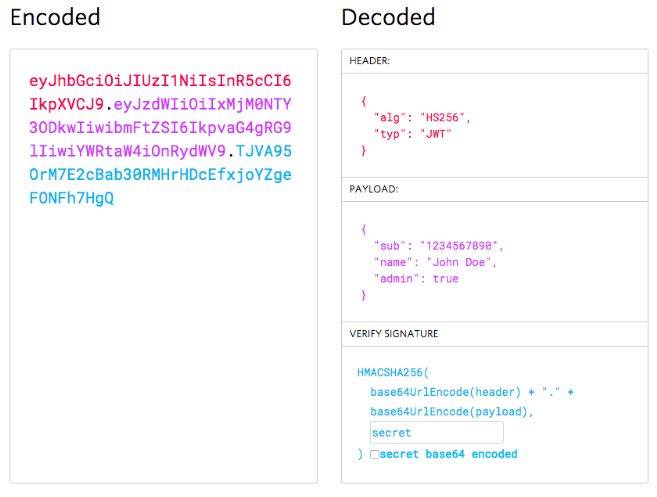
\includegraphics[width=0.6\textwidth]{jwt-beispiel.png}
  
  
\raggedleft
    \footnotesize\sffamily\textbf{Quelle:} \url{https://jwt.io/introduction} am 27. April 2023
  \caption{Beispiel eines verschlüsselten Tokens von JWT}
  \label{fig:jwt-example}
\end{figure}
        \subsubsection{Chakra UI}
        \label{sec:chakraUI}
Chakra UI ist eine simple Komponenten Bibliothek, welche das designen von React Anwendungen vereinfacht\footnote{Quelle: \url{https://chakra-ui.com/} am 22. April 2023}. Es stellt Komponenten zur Verfügung, welchen verschiedene Attribute zugeordnet werden können um diese nach eigenem ermessen zu designen (siehe Code Beispiel \ref{lst:chakra-example} und Abbildung \ref{fig:chakra-example}).


  \begin{figure}[h]
  \centering
  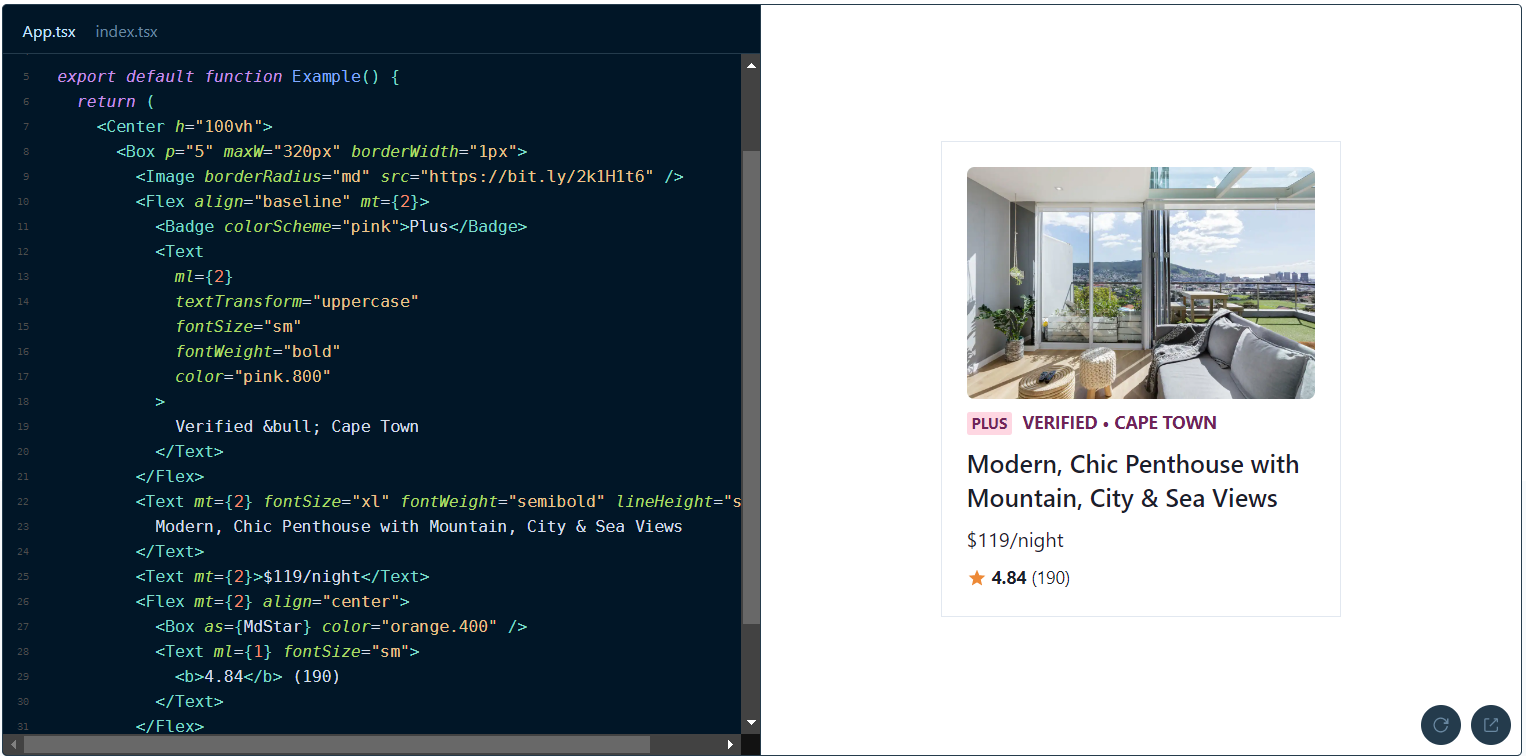
\includegraphics[width=0.4\textwidth]{Chakra-UI Beispiel.png}
  
\raggedleft
    \footnotesize\sffamily\textbf{Quelle:} \url{https://chakra-ui.com/} am 27. April 2023
  \caption{Darstellung der mit Chakra UI designten React Komponente aus dem Code Beispiel \ref{lst:chakra-example}}
  \label{fig:chakra-example}
\end{figure}
  

\begin{lstlisting}[style=codeStyle, caption={Beispiel mit Chakra UI designten React Komponente (siehe Abbildung  \textbf{Quelle:} \url{https://chakra-ui.com/} am 27. April 2023}, label={lst:chakra-example}]
import * as React from "react";
import { Box, Center, Image, Flex, Badge, Text } from "@chakra-ui/react";
import { MdStar } from "react-icons/md";

export default function Example() {
  return (
    <Center h="100vh">
      <Box p="5" maxW="320px" borderWidth="1px">
        <Image borderRadius="md" src="https://bit.ly/2k1H1t6" />
        <Flex align="baseline" mt={2}>
          <Badge colorScheme="pink">Plus</Badge>
          <Text
            ml={2}
            textTransform="uppercase"
            fontSize="sm"
            fontWeight="bold"
            color="pink.800"
          >
            Verified &bull; Cape Town
          </Text>
        </Flex>
        <Text mt={2} fontSize="xl" fontWeight="semibold" lineHeight="short">
          Modern, Chic Penthouse with Mountain, City & Sea Views
        </Text>
        <Text mt={2}>$119/night</Text>
        <Flex mt={2} align="center">
          <Box as={MdStar} color="orange.400" />
          <Text ml={1} fontSize="sm">
            <b>4.84</b> (190)
          </Text>
        </Flex>
      </Box>
    </Center>
  );
}
\end{lstlisting}
        \subsubsection{Formik und Yup}
        \label{sec:formik}
Formik ist die beliebteste Open-Source-Bibliothek für Formulare in React \footnote{Quelle: \url{https://formik.org/} am 22. April 2023}. Sie vereinfacht die Handhabung von Formularen und bietet Funktionen wie Validierung der eingegebenen Werte, Fehlermeldungen und Unterstützung für mehrstufige Formulare.

Yup ist eine Bibliothek  zur einfachen Definition von Schemata, die von bestimmten Formularen erfüllt werden sollen. Sie ermöglicht die Erstellung komplexer Schemata mit wenig Code\footnote{Quelle: \url{https://github.com/jquense/yup} am 22. April 2023}.

Die Integration von Yup-Schemata in Formik-Formularen ist bereits unterstützt, was eine einfache Handhabung von Überprüfungen und Fehlerbehandlungen bei Benutzereingaben ermöglicht.

        \subsubsection{chess.js}
        \label{sec:chess.js}
chess.js ist eine Schach Bibliothek, welche die gesamte Schachlogik zur Verfügung stellt\footnote{Quelle: \url{https://github.com/jhlywa/chess.js/} am 22. April 2023}. Es bietet Methoden, welche alle aktuell möglichen Züge ausgibt, einen Zug ausführt und verschiedene Notationen des Zuges zurückgibt, überprüft ob es sich um ein Schachmatt oder Patt handelt, eine Partie mittels einer FEN\footnote{Quelle: \url{https://de.wikipedia.org/wiki/Forsyth-Edwards-Notation} am 22. April 2023} oder PGN\footnote{\url{https://de.wikipedia.org/wiki/Portable_Game_Notation} am 22. April 2023} Notation laden kann und vieles weitere. 
        \subsubsection{chessground}
        \label{sec:chessground}
chessground ist ein Open-Source-Schach-User-Interface, das ursprünglich für die Online-Schachplattform \url{lichess.org} entwickelt wurde\footnote{Quelle: \url{https://github.com/lichess-org/chessground} am 22. April 2023}. Es bietet zahlreiche Konfigurationsmöglichkeiten, wie zum Beispiel Animationen beim bewegen von Figuren, Auswahl der anklickbaren und bewegbaren Figuren, Anpassung des Figurendesigns und vieles mehr. Die eigentliche Schachlogik ist nicht enthalten, sodass verschiedene Schachvarianten mit Sonderregelungen implementiert werden können.

\subsubsection{bcrypt}
\label{sec:bcrypt}
bcrypt ist eine Bibliothek welche entwickelt wurde um Passwörter zu verschlüsseln. Es basiert auf Blowfish, einem Verschlüsselungsalgorithmus, und löst das Problem, dass durch schnellere Hardware Passwörter immer schneller kodiert und dekodiert werden können und dadurch Sicherheitsrisiken entstehen. Es löst dieses Problem dadurch, dass es die Passwörter um einen selbst definierbaren Faktor zeitlich länger kodiert indem es mehrere Iterationen durchführt\footnote{Quelle: \url{https://auth0.com/blog/hashing-in-action-understanding-bcrypt/}}.
        
	\newpage
\newpage\thispagestyle{empty}\hspace{1em}\newpage
       
\chapter{Systemarchitektur und Konzeption}
In diesem Kapitel wird die Systemarchitektur der Anwendung vorgestellt, indem erläutert wird wie die verschiedenen Komponenten und Technologien zusammenarbeiten und miteinander kommunizieren. Die vorhandenen Funktionen der Schach-App werden mit Bildschirmfotos und Erklärungen veranschaulicht. Des weiteren werden verschiedene Abläufe durch Aktivitäts- und Sequenzdiagramme verdeutlicht.
\section{Einführung}
Die Anwendung ist in zwei Hauptkomponenten unterteilt: das Frontend und das Backend. Das Frontend ist für die Darstellung der Benutzeroberfläche und die Interaktion mit dem Benutzer verantwortlich, während das Backend die Spiellogik, die Verwaltung der Benutzerdaten und die Echtzeit-Kommunikation zwischen den Spielern steuert.

Die Anwendung verwendet moderne Web-Technologien, um eine reaktive und benutzerfreundliche Oberfläche zu schaffen. Das Frontend basiert auf dem React-Framework (siehe Kapitel \ref{sec:react}), das es ermöglicht, wiederverwendbare Komponenten zu entwickeln und den Anwendungsstatus effizient zu verwalten. Das User-Interface basiert auf Chakra UI (siehe Kapitel \ref{sec:weiteres}, einem modernen und flexiblen Komponenten-Bibliothekssystem, das die Entwicklung von responsiven und zugänglichen Benutzeroberflächen erleichtert. Die Benutzerführung und die Kommunikation zwischen den React-Komponenten sind so gestaltet, dass sie eine nahtlose und intuitive Benutzererfahrung bieten.

Auf der Backend-Seite wird Node.js mit dem Express-Framework (siehe Kapitel \ref{sec:express}) verwendet, um einen leistungsstarken und skalierbaren Server bereitzustellen. Die API-Endpunkte und die Echtzeitkommunikation mittels Socket.io (siehe Kapitel \ref{sec:socket.io}) ist so konzipiert, dass sie den Anforderungen der verschiedenen Frontend-Komponenten gerecht werden und die Kommunikation zwischen Frontend und Backend erleichtern. Für die Speicherung und Verwaltung der Benutzerdaten zum Anmelden wird eine PostgreSQL-Datenbank  (siehe Kapitel \ref{sec:Postgresql}) verwendet, die aufgrund ihrer Leistungsfähigkeit und Flexibilität ausgewählt wurde. Freundeslisten und Daten aktiver Spiele werden in einer Redis-Datenbank gespeichert, die sich durch hohe Leistung und niedrige Latenz auszeichnet, insbesondere bei Lese- und Schreibvorgängen. Redis, eine In-Memory-Datenstruktur, eignet sich ideal für Anwendungen, bei denen schnelle Zugriffszeiten und Skalierbarkeit wichtig sind. Die Kombination von PostgreSQL und Redis ermöglicht eine effiziente Verwaltung sowohl persistenter als auch flüchtiger Daten und fördert eine optimale Benutzererfahrung.
\section{Architekturübersicht}
Das Komponentendiagramm in Abbildung \ref{fig:Komponentendiagramm} visualisiert den Zusammenhang der Hauptkomponenten für die Kommunikation.

Wie zu erkennen ist, sind die Datenbanken und deren Funktionen getrennt gehalten. Die Web-API und die PostgreSQL Datenbank werden zum Authentifizieren genutzt, währen die Kommunikation mittels Socket.io und die Redis Datenbank für die restlichen Funktionen der Anwendung verwendet werden. Dies erhöht die Modularität und Flexibilität, wodurch die verschiedenen Datenbanken und Funktionen unabhängig voneinander entwickelt, gewartet und skaliert werden können.

Im Frontend gibt es drei Komponenten, welche die Web-API verwenden: Der \textit{UserContext}, \textit{Login} und \textit{SignUp}. Die Web-API verwendet dabei nur die Methoden GET und POST. Der \textit{UserContext} ist verantwortlich für die Verwaltung des Benutzerzustands, während die Komponenten \textit{Login} und \textit{SignUp} das setzen des Benutzerzustands über das Anmelden und Registrieren unterstützen. Der \textit{SocketContext} baut die Socket.io Verbindung für die Echtzeitkommunikation auf und stellt sie den restlichen React Komponenten zur Verfügung, um Events zu senden und zu empfangen.

Die Anfragen über die Web-API werden durch den in \textit{authRouter} definierten Express Router entgegengenommen. Zur Behandlung werden in ihm verschieden Middlewares der Datei \textit{authController} für verschiedene Anfragen festgelegt, welche auf die PostgreSQL Datenbank zugreifen. Die Web-API und die PostgreSQL Datenbank werden lediglich für das Registrieren und Anmelden von Benutzern verwendet.

Beim Herstellen einer Socket.io Verbindung in \textit{SocketContext} werden im Backend die Middlewares aus \textit{socketMiddleware} ausgeführt, welche unter anderem die Listener aus \textit{socketController} und \textit{socketChessContoller} initialisieren. Der Unterschied zwischen den Listenern der beiden Dateien ist, dass \textit{socketController} sich um allgemeine Funktionen wie das Versenden von Freundschaftsanfragen oder das senden von Informationen an das Frontend kümmert, während \textit{socketChessController} Listener enthält, welche sich um Funktionen des Schachspiels kümmert, wie zum Beispiel das Behandeln eines neuen Zugs. 

Alle Dateien im \verb|sockets| Package verwenden den \textit{redisController}, um Daten aus der Redis Datenbank abzurufen und zu speichern. Beispielsweise werden Freundschaftsanfragen, Freunde und Daten aktiver Spiele in der Redis Datenbank von dem \textit{redisController} verwaltet, abgerufen und gespeichert.

\begin{figure}[h!]
\centering
\begin{adjustbox}{width=\textwidth}
\begin{tikzpicture}
 \begin{umlpackage}[x=4]{Frontend}
 \begin{umlcomponent}{UserContext}
 \begin{umlcomponent}{SocketContext}
 \umlbasiccomponent{Login}
 \umlbasiccomponent[x=3]{SignUp}
 \end{umlcomponent}
 \end{umlcomponent}
 \end{umlpackage}
 
 
 \begin{umlpackage}[y=-5]{Backend}
 \begin{umlpackage}{sockets}
 \umlbasiccomponent{socketController}
 \umlbasiccomponent[x=5]{socketChessController}
 \umlbasiccomponent[x=2.5, y=-2.5]{socketMiddleware}
 \end{umlpackage}
 \umlbasiccomponent[x=2.5, y=-5]{redisController}
 \umlbasiccomponent[x=10]{authRouter}
 \umlbasiccomponent[x=10, y=-5]{authController}
 \end{umlpackage}
 
\umlHVassemblyconnector[with port, anchor2=130]{SocketContext}{sockets}

\umlHVassemblyconnector[with port]{UserContext}{authRouter}
\umlVHVassemblyconnector[with port, anchor1=-90]{Login}{authRouter}
\umlVHVassemblyconnector[with port, anchor1=-90]{SignUp}{authRouter}

\umlnote[x=-1,y=2]{SocketContext-west-port}{socket.io-client}
\umlnote[x=12, y=2]{UserContext-east-port}{Web-API}
\umlnote[x=12, y=-1]{authRouter-north-port}{Express Router}
 
 \umlbasiccomponent[x=2.5, y=-13]{Redis DB}
 \umlbasiccomponent[x=10, y=-13]{PostgreSQL DB}
 
\umlassemblyconnector[anchor1=-90, anchor2=90]{authRouter}{authController} 
\umlVHassemblyconnector[anchor1=-90, anchor2=-180]{socketController}{redisController}
\umlVHassemblyconnector[anchor1=-90, anchor2=0]{socketChessController}{redisController}
\umlVHassemblyconnector[anchor1=-90, anchor2=90]{socketMiddleware}{redisController}

 
 \umlassemblyconnector[with port, anchor1=-90, anchor2=90]{authController}{PostgreSQL DB}
  \umlassemblyconnector[with port, anchor1=-90, anchor2=90]{redisController}{Redis DB}
\end{tikzpicture}
\end{adjustbox}
\caption{Komponentendiagramm der Anwenundung}
\label{fig:Komponentendiagramm}
\end{figure}

\section{Konzeption der Schachuhren}
\label{sec:Konzept-Schachuhr}
Bei der Konzeption der Schachuhren war ein Aspekt besonders entscheidend: Was passiert, falls ein Spieler vorübergehend keine Internetverbindung beim senden oder beim empfangen von Events hat?

Um den Server zu entlasten wäre natürlich eine Client basierte Lösung ideal, bei der mit einem Zug auch die jeweilige aktuelle Zeit gesendet wird. Wenn ein Spieler allerdings eine schlechte Internetverbindung hat und deshalb der Zug im Backend und bei dem anderen Spieler erst verspätet ankommt können sich die Zeiten der beiden Spieler erheblich unterscheiden. Es stellt sich die Frage, welche dieser Zeiten jetzt gültig ist. Trivialerweise entsteht das gleiche Problem bei einer verzögerten Zustellung. Wenn die Zeit auf einem Client bereits abgelaufen wäre, könnte sie auf dem anderen noch weiterlaufen. Hat der Spieler dann gewonnen oder nicht?

Um dieses Problem zu umgehen liegt die einfachste Lösung darin, eine serverseitige Schachuhr einzuführen. Diese Uhr bestimmt die aktuellen Zeiten. Wenn ein Zug im Backend ankommt, wird die auf dem Server gültige Zeit an die Clients gesendet. Dadurch gibt es keine Unklarheiten hinsichtlich der aktuellen Zeit. Wenn eine Zeit auf dem Server abläuft wird dies durch ein Event mitgeteilt.  Es kann zwar vorkommen, dass bei den Clients zu dem Zeitpunkt noch Zeit übrig ist, wenn das letzte Event aufgrund einer schlechten Verbindung verspätet eingetroffen ist, aber dieses Problem ist unvermeidbar.

Durch dieses Konzept umgeht man auch das Problem, dass Client seitiger Code im Browser manipulierbar sein kann und dadurch die Schachuhren beeinflussbar wären.

Wie die Schachuhren konkret funktionieren wird in den nachfolgenden Kapiteln behandelt.

    \section{Frontend-Architektur}
Das Frontend der Anwendung wurde unter Verwendung von React (Abschnitt \ref{sec:react}), Socket.io (Abschnitt \ref{sec:socket.io}) und weiteren Bibliotheken aus Abschnitt \ref{sec:weiteres} entwickelt.



In diesem Kapitel werde ich die unterschiedlichen React-Komponenten vorstellen und erläutern, wie sie zusammenarbeiten, um bestimmte Funktionen zu erfüllen und sowohl untereinander als auch mit dem Backend kommunizieren.

\begin{figure}[h!]
\centering

\begin{minipage}{0.5\textwidth}
\dirtree{%
.1 client/.
.2 public/.
.3 Gambit dark.png.
.3 Gambit light.png.
.3 Gambit springer.png.
.3 index.html.
.3 manifest.json.
.3 robots.txt.
.2 src/.
.3 components/.
.4 ActiveGames.js.
.4 AddFriendModal.js.
.4 Chat.js.
.4 ChessClock.js.
.4 Friend.js.
.4 FriendList.js.
.4 FriendRequest.js.
.4 GameRequests.js.
.4 Navbar.js.
.4 PromotionModal.js.
.3 contexts/.
.4 AccountContext.js.
.4 SocketContext.js.
.4 tests/.
.3 themes/.
.4 Theme.js.
.3 utils/.
.4 ChessLogic.js.
.3 views/.
.4 ChessGame.js.
.4 Home.js.
.4 Login.js.
.4 Signup.js.
.3 App.js.
.3 index.js.
.3 Views.js.
.2 package.json.
}
\end{minipage}
\caption{Ordnerstruktur des Frontends}
\label{fig:frontend_dirtree}

\end{figure}

Die Ordnerstruktur (Abbildung \ref{fig:frontend_dirtree}) ist wie folgt aufgebaut:
\begin{itemize}
\item \textbf{public:} In diesem Ordner befinden sich statische Ressourcen, wie zum Beispiel Bilder des Logos, die von der Anwendung verwendet werden.
\item \textbf{components:} Dieser Ordner enthält alle React-Komponenten, die für die Anwendung verwendet werden. Sie sind modular und stellen jeweils nur ein Teil eines User Interfaces dar.
\item \textbf{contexts:} Hier befinden sich die React Contexts, die zum Verwalten von globalen Zuständen und Kommunikationsschnittstellen verwendet werden.
\item \textbf{themes:} Dieser Ordner enthält Dateien, die für das Design und die Anpassung des Aussehens der Anwendung mittels Chakra UI verantwortlich sind.
\item \textbf{utils:} In diesem Ordner befinden sich Hilfsdateien, die ausgelagerte Funktionen zur Verfügung stellen.
\item \textbf{views:} Dieser Ordner enthält die verschiedenen Seiten der Anwendung. Zu diese Seiten kann mit Hilfe des React-Routers über verschiedene Pfade navigiert werden. Diese Seiten verwenden teilweise die Komponenten aus dem components-Ordner, um eine vollständige Benutzeroberfläche darzustellen.
\end{itemize}
    
        \subsection{React-Komponenten}
        \label{sec:React-Komponenten}
Der hierarchische Aufbau der React-Komponenten in Abbildung \ref{fig:frontend_tikz} zeigt die Struktur und Verschachtelung der Anwendung für angemeldete Benutzer. Nicht angemeldete Benutzer sehen lediglich die Komponenten ActiveGames und FriendList nicht, während der restliche Aufbau gleich bleibt. In diesem Abschnitt werden die wichtigsten Komponenten und ihre Funktionen innerhalb der Anwendung erläutert.
        
\begin{itemize}
\item \textbf{AccountContext:} Stellt Informationen über den Benutzerstatus allen Folgenden Komponenten mittels eines React-Contexts zur Verfügung. Diese Informationen beinhalten, ob ein Benutzer angemeldet ist und falls er das ist seinen Benutzernamen.
\item \textbf{SocketContext:} In diesem React Context wird eine Socket.io Verbindung mit dem Server hergestellt und allen darauf folgenden Komponenten bereitgestellt.
\item \textbf{ChakraBaseProvider und ColorModeScript:} Diese importierten Komponenten von ChakraUI stellen die Funktionen zum designen bereit. Dazu gehören Beispielsweise das Verwenden des globalen Zustands des Farbenschemas (dunkel oder hell) oder das Zugreifen auf definierte Stile.
\item \textbf{Views:} Diese Komponente beinhaltet das User Interface. Mit Hilfe des React-Routers werden hier die Komponenten des \verb|view|-Ordners unter einem bestimmten Pfad definiert. Des weiteren beinhaltet es die Komponenten GameRequest und Navbar, welche durch die Definition in dieser Komponente auf jedem Pfad vorhanden sind.
\begin{itemize}
\item \textbf{Navbar:} Die Navigationsleiste besteht aus dem Logo und einem Button zum wechseln des Farbschemas. Je nachdem, ob ein Benutzer angemeldet ist oder nicht beinhaltet es noch Buttons zum Anmelden, Registrieren oder Abmelden (siehe Abbildungen \ref{fig:home-not-logged-in} \& \ref{fig:home-logged-in}).
\item \textbf{GameRequests:} Diese Komponente ist dafür Verantwortlich beim Eingang einer Spielanfrage eines Freundes, dieses als Modal darzustellen und bietet die Möglichkeit diese Anfrage zu beantworten (siehe Abbildung \ref{fig:game-request}).
\end{itemize}
\item \textbf{Home:} Diese Komponente stellt die Startseite dar und enthält die Buttons zum Starten eines Spiels mit verschiedenen Schachuhr Konfigurationen (siehe Abbildung \ref{fig:home-not-logged-in}). Diese Buttons sind in einigen online Schachplattformen (Beispielsweise \url{lichess.org}) bereits gängig und benötigen keine zusätzliche Erklärung. Ist ein Benutzer angemeldet sind auch noch die Komponenten ActiveGames und FriendList auf der rechten Seite vorhanden (siehe Abbildung \ref{fig:home-logged-in}).
\begin{itemize}
\item \textbf{ActiveGames:} ActiveGames ist eine Komponente die alle derzeit aktiven Spiele mit den Informationen der Benutzernamen und wer welche Farbe spielt als Buttons darstellt (siehe Abbildung \ref{fig:home-logged-in}). Beim klicken auf einen dieser Buttons wird zu der aktiven Partie navigiert.
\item \textbf{FriendList:} Diese Komponente verwaltet alle Freunde und Freundschaftsanfragen eines Benutzers, während die Darstellung und Interaktion die Unterkomponenten \textit{Friend} und \textit{FriendRequest} übernehmen. Die Funktionsweise der Komponente mit seinen Unterkomponenten wird in Abschnitt \ref{sec:Friends} erläutert.
\begin{itemize}
\item \textbf{Friend:} Übernimmt die Darstellung eines Freundes. Mittels eines farbigen Punktes ist erkennbar, ob dieser Freund gerade online ist (grün) oder nicht (rot) (siehe Abbildung \ref{fig:home-logged-in}). Ist er online erscheint noch mindestens ein weiterer Button. Es beinhaltet ein Icon in Form von gekreuzten Schwertern und einem Schild. Dies hat die Funktion einen Freund zu einem Spiel herauszufordern. Falls dieser Freund gerade ein aktives Spiel hat erscheint noch ein zweiter Button mit einem Auge als Icon, welches den Benutzer zu dem aktiven Spiel des Freundes als Zuschauer navigiert.
\item \textbf{FriendRequest:} Eine Freundschaftsanfrage wird mittels dieser Komponente dargestellt und beantwortet (siehe Abbildung \ref{fig:home-logged-in}).
\item \textbf{AddFriendModal:} Mit Hilfe dieser Komponente können Freundschaftsanfragen unter Angabe des Benutzernamens versendet werden (siehe Abbildung \ref{fig:AddFriendModal}.
\end{itemize}
\end{itemize}

\item \textbf{Login \& SignUp:} Komponenten, die das Anmelden und Registrieren mittels Formularen mit Formik und Yup (siehe Abschnitt \ref{sec:formik}) ermöglichen und mit dem Server zur Authentifizierung kommunizieren (siehe Abbildungen \ref{fig:SignUp} \& \ref{fig:Login}). Diese Komponenten befinden sich unter dem Pfad \verb|/login|, beziehungsweise \verb|/signup|.
\item \textbf{ChessGame:} Die Komponente ChessGame ist das Herzstück der Anwendung, da dort das eigentliche Schachspiel stattfindet. Die ChessGame Komponente wird durch den Pfad \verb|/game/:roomId| gerendert und holt sich durch die roomId die Spieldaten vom Backend. In der Abbildung \ref{fig:chess-game} ist eine beispielhafte Komponente zu sehen. Auf der rechten Seite neben dem Brett befindet sich die \textit{ChessClock} Komponente und daneben befindet sich die \textit{Chat} Komponente. Das Spielfeld und die Figuren entstehen durch die Bibliothek chessground, während die Spiellogik hinter dem Schachspiel von chess.js verwaltet wird (siehe Abschnitt \ref{sec:chess.js}). Eine detaillierte Beschreibung, was in der Komponente beim spielen oder empfangen eines Zugs passiert befindet sich im Abschnitt \ref{sec:Schachspiel}.



\begin{itemize}
\item \textbf{ChessClock:} ChessClock ist eine Komponente, die die Verwaltung und Darstellung der Schachuhren übernimmt.
\item \textbf{Chat:} Die Chat Komponente repräsentiert einen simplen gehaltenen Chat in dem die beiden Spieler kommunizieren können. Zuschauer können ihn lesen, allerdings nichts selber schreiben, da sie Tipps geben könnten.
\item \textbf{PromotionModal:} Über dieses Modal lässt sich bei einer Bauernumwandlung eine Figur auswählen, welche den Bauern ersetzen soll (siehe Abbildung \ref{fig:PromotionModal}).
\end{itemize}
\end{itemize}
 
\begin{figure}[h!]
        \centering
        
\begin{adjustbox}{width=\textwidth}
        \begin{tikzpicture}
\node {App}
    child {node {AccountContext}
    		child {node {SocketContext}
    			child {node {ChakraBaseProvider} [sibling distance = 2.5cm]
    				child {node [xshift= -2cm] {ColorModeScript}}
    					child {node {Views} [sibling distance = 2.6cm]
    						child {node {Home} edge from parent [dashed]					
    							child {node {ActiveGames} edge from parent [solid]}
    							child {node {FriendList} [sibling distance = 2.0cm] edge from parent [solid]
								child {node {Friend}}
    								child {node {...}}
    								child {node {FriendRequest}}
    								child {node {...}}
    								child {node {AddFriendModal}}    							
    							 }
    						}
    						child {node {Login} edge from parent [dashed]}  
    						child {node {SignUp} edge from parent [dashed]}  				
    						child {node {ChessGame} edge from parent [dashed]
						child {node {ChessClock} edge from parent [solid]}
						child {node {Chat} edge from parent [solid]}    			
						child {node {PromotionModal} edge from parent [solid]}			
    						}
						child {node {GameRequests}}
						child {node {Navbar}}  
    					}
    				} 
    			}
    		};
    		

    \node[anchor=north east, xshift=-7cm] (dashed) at (current bounding box.north east) {};
    \draw[dashed] (dashed.east) -- ++(0.8cm, 0);

    \node[anchor=west, right=1cm of dashed] {Route Komponenten};

    \node[below=0.3cm of dashed] (solid) {};
    \draw[solid] (solid.east) -- ++(0.8cm, 0);

    \node[anchor=west, right=1cm of solid] {enthaltene Unterkomponenten};
\end{tikzpicture}
\end{adjustbox}
    	
\caption{Aufbau der React-Komponenten für angemeldete Benutzer}
\label{fig:frontend_tikz}
        
        \end{figure}

  \begin{figure}[htbp]
  \centering
  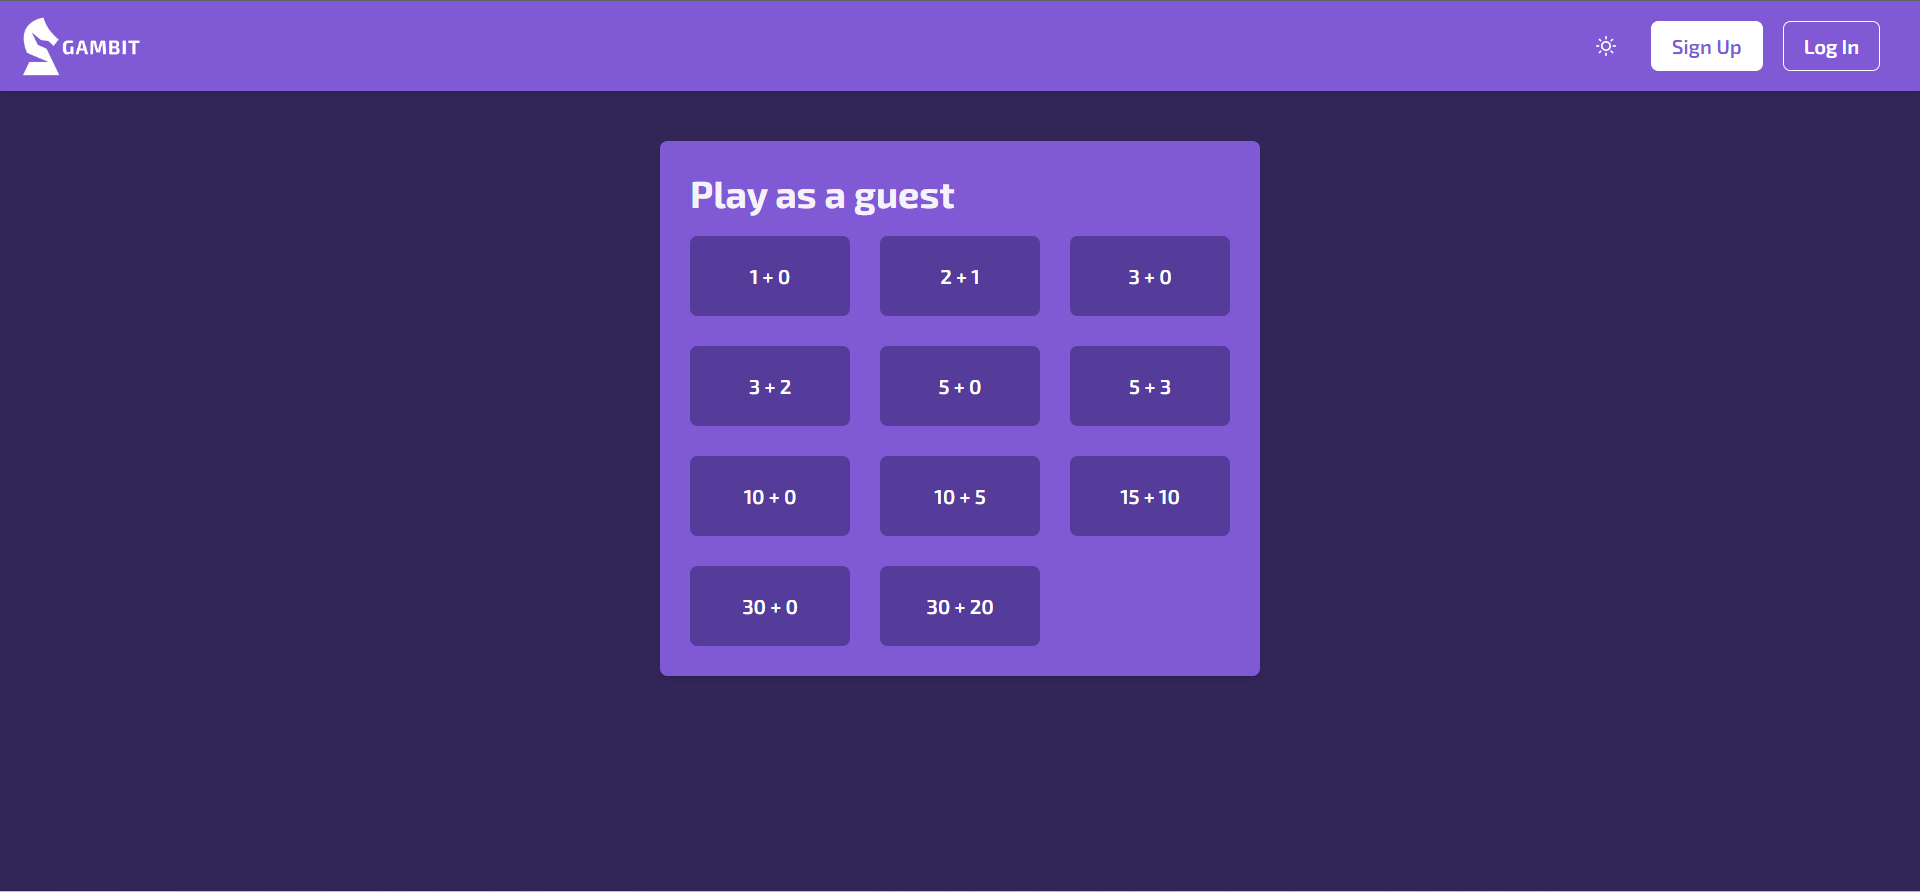
\includegraphics[width=\textwidth]{Home_not_logged_in.png}
  \caption{Home und Navbar Komponente eines nicht angemeldeten Benutzers im dunklen Farbschema}
  \label{fig:home-not-logged-in}
\end{figure}

  
    \begin{figure}[htbp]
    \centering
  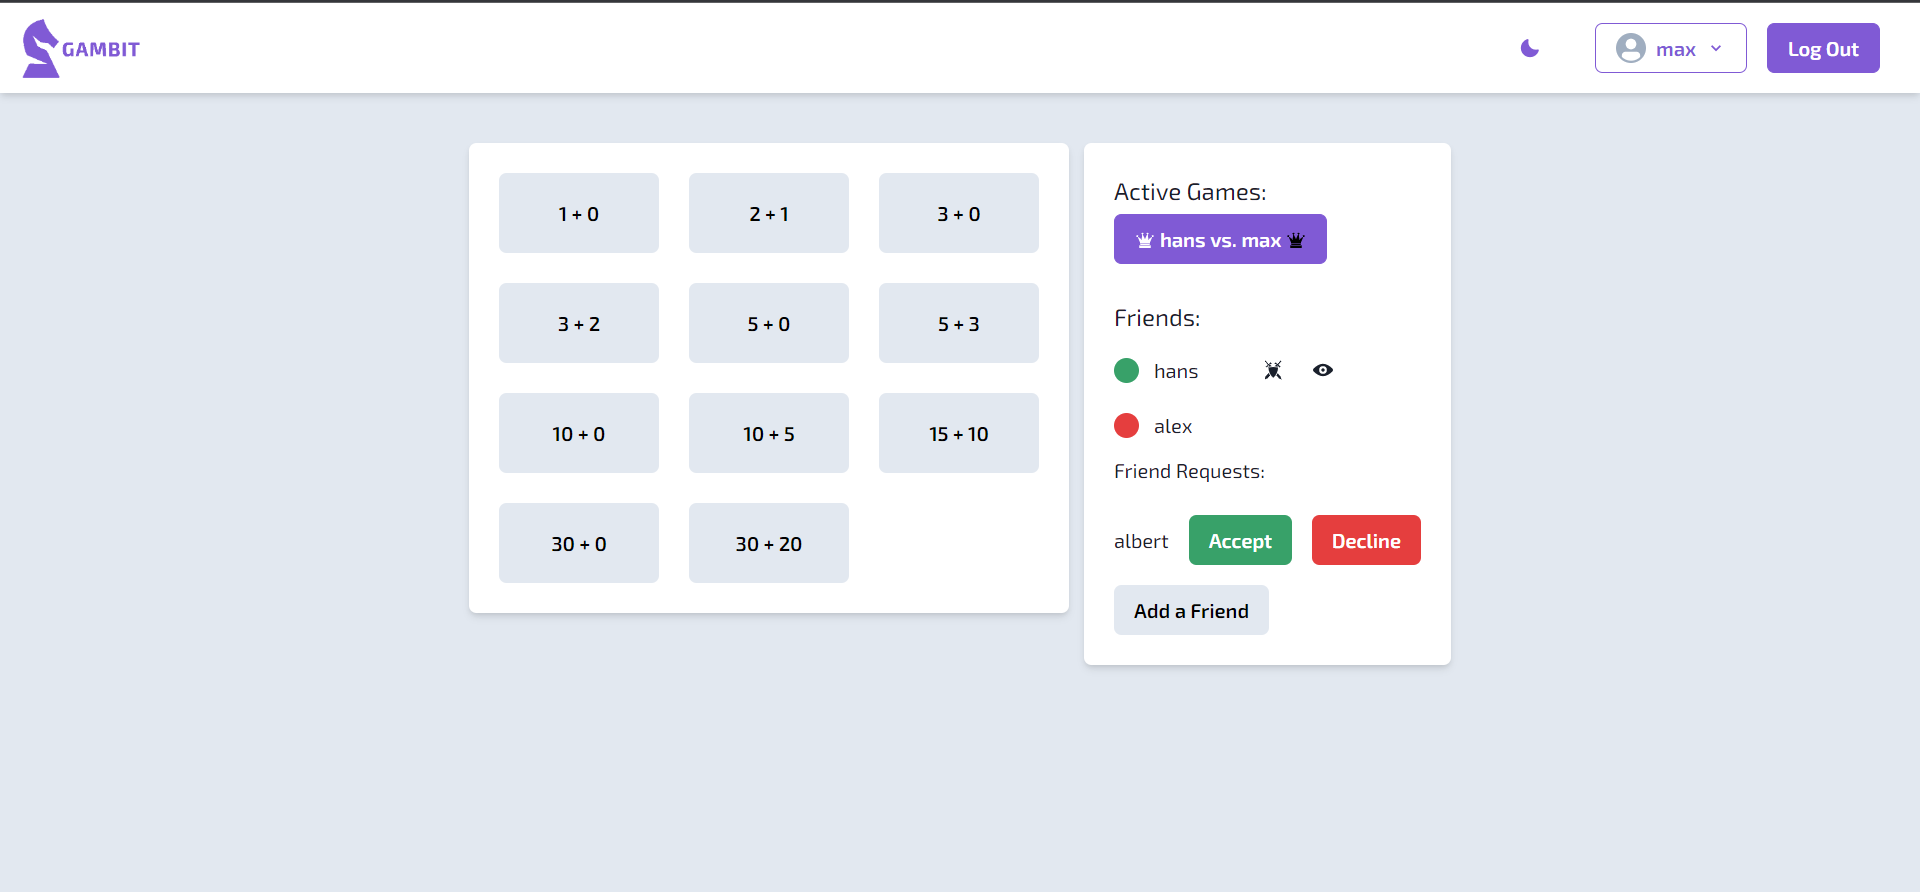
\includegraphics[width=\textwidth]{Home_logged_in.png}
  \caption{Home und Navbar Komponente eines angemeldeten Benutzers im hellen Farbschema}
  \label{fig:home-logged-in}
\end{figure}

      \begin{figure}[htbp]
      \centering
  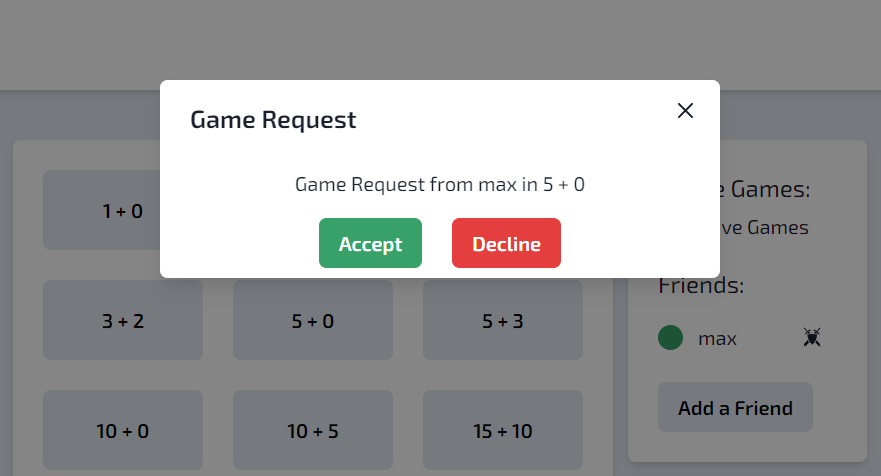
\includegraphics[width=0.7\textwidth]{game_request.png}
  \caption{Das Modal der Komponente GameRequest in hellem Farbschema}
  \label{fig:game-request}
\end{figure}


      \begin{figure}[htbp]
      \centering
  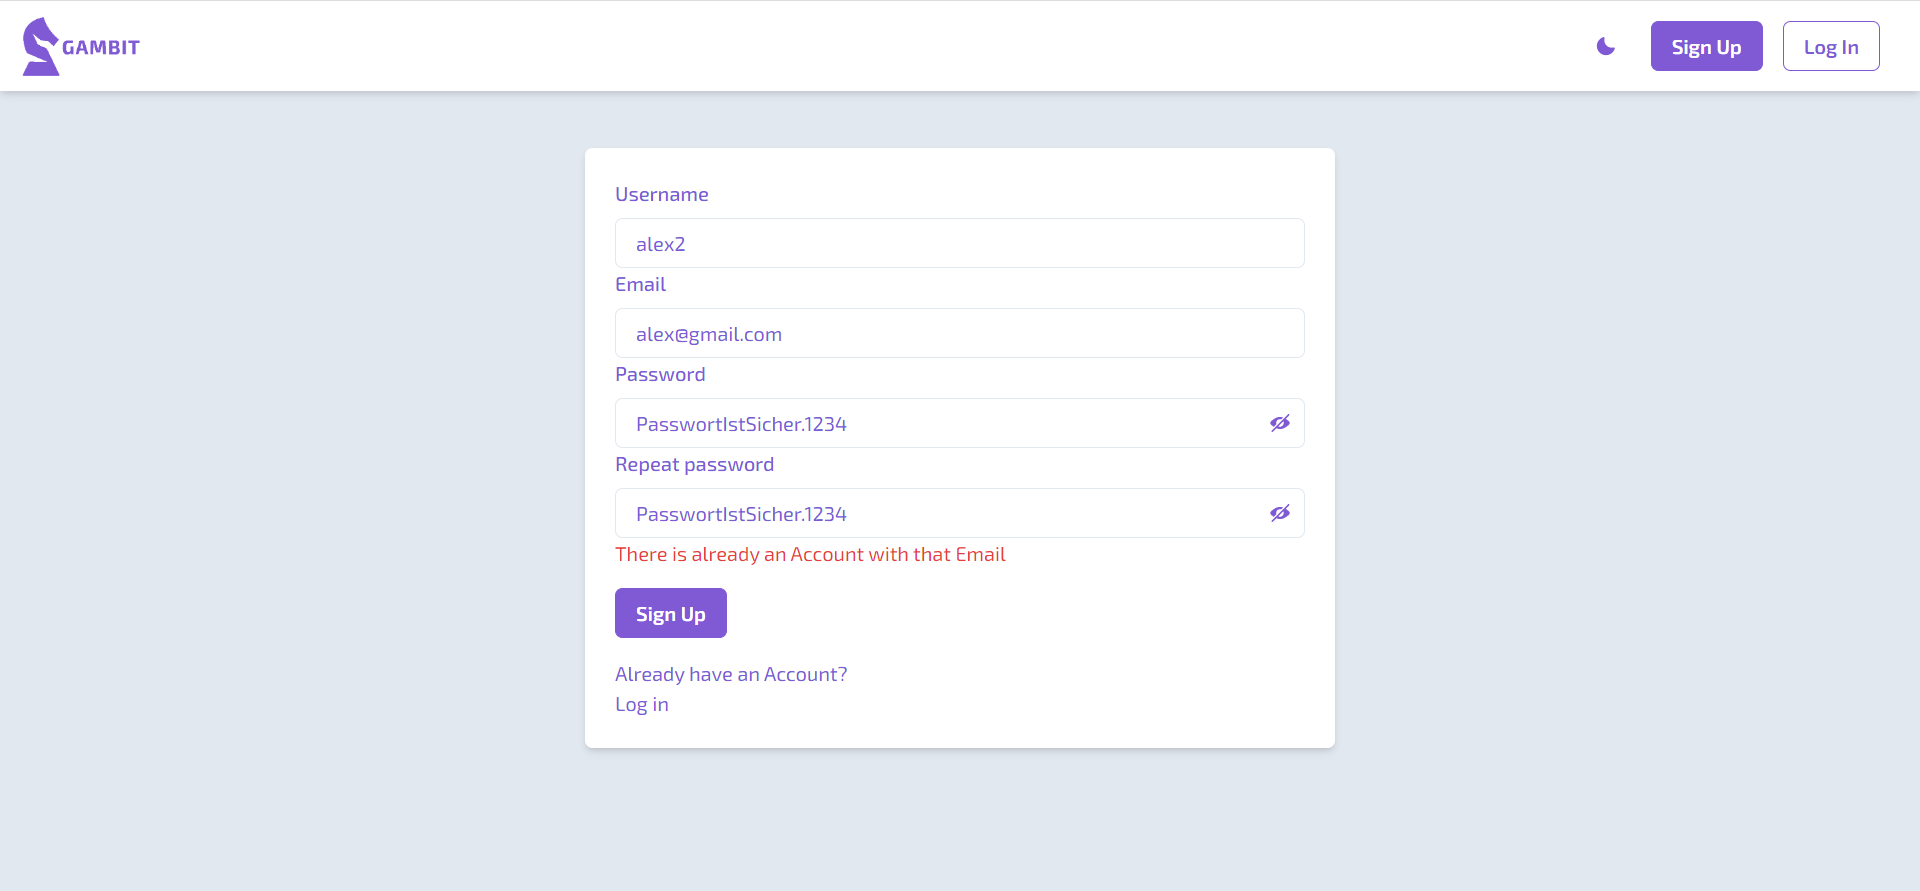
\includegraphics[width=\textwidth]{SignUp.png}
  \caption{Beispiel einer SignUp-Komponente mit bereits verwendet E-Mail Adresse} 
  \label{fig:SignUp}
\end{figure}

      \begin{figure}[htbp]
      \centering
  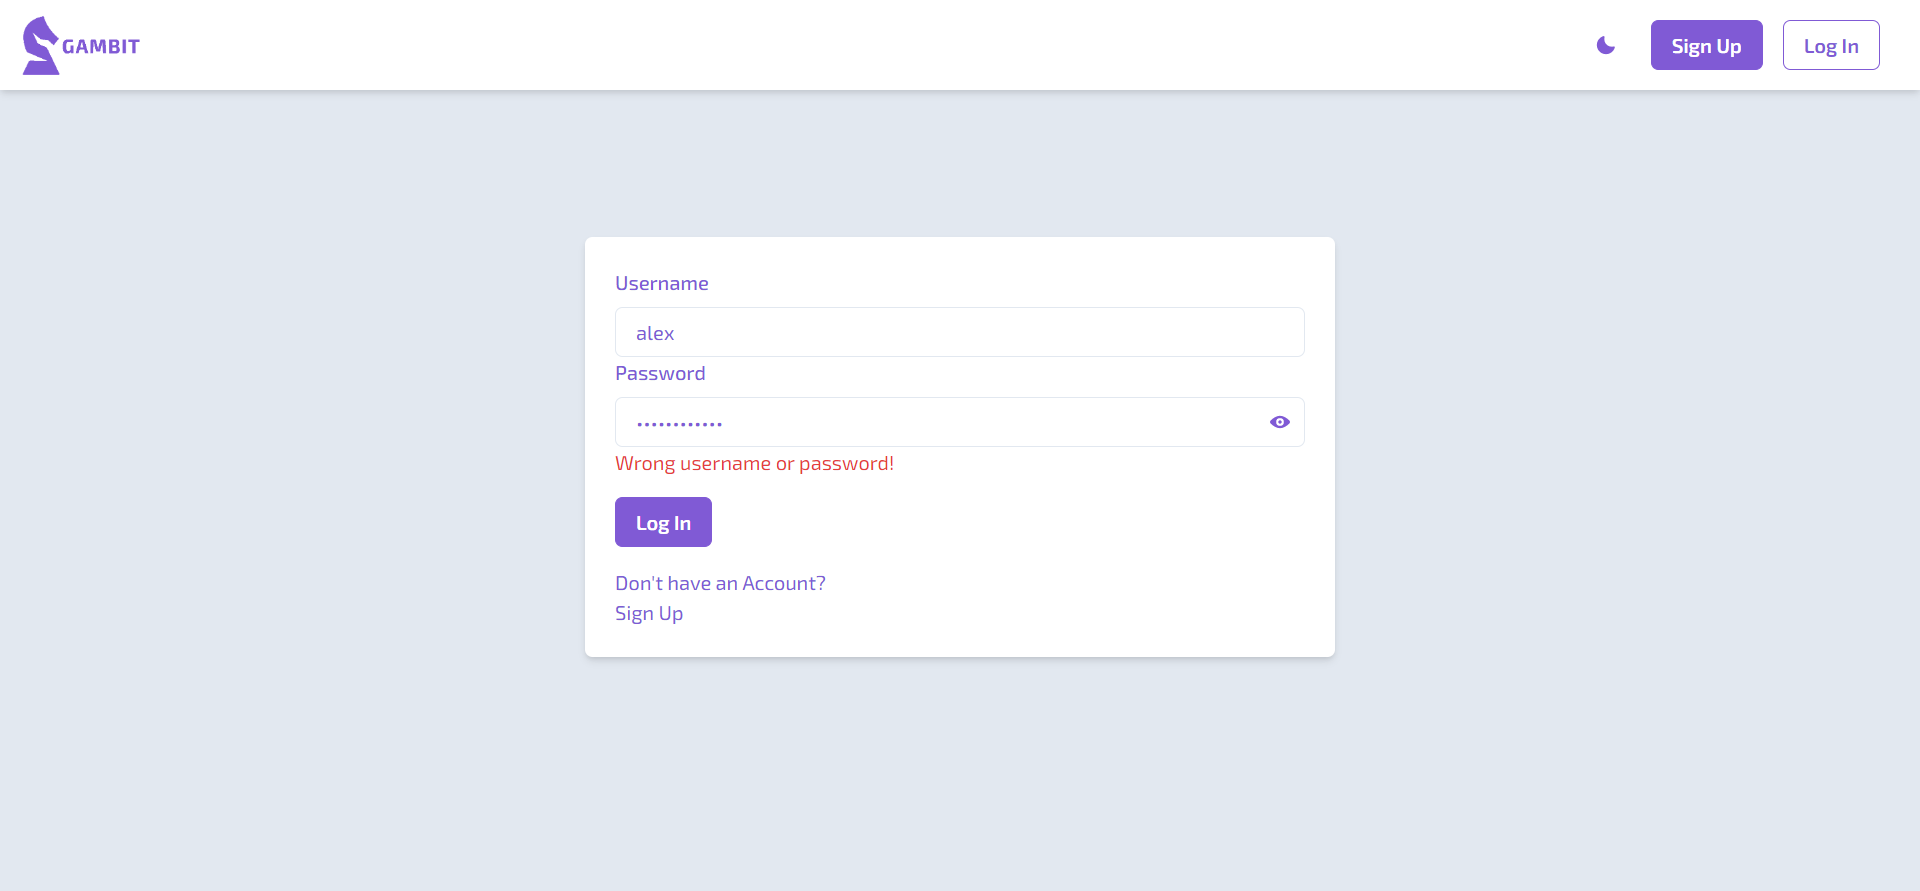
\includegraphics[width=\textwidth]{Login.png}
  \caption{Beispiel einer Login-Komponente mit ungültigen Daten} 
  \label{fig:Login}
\end{figure}

      \begin{figure}[htbp]
      \centering
  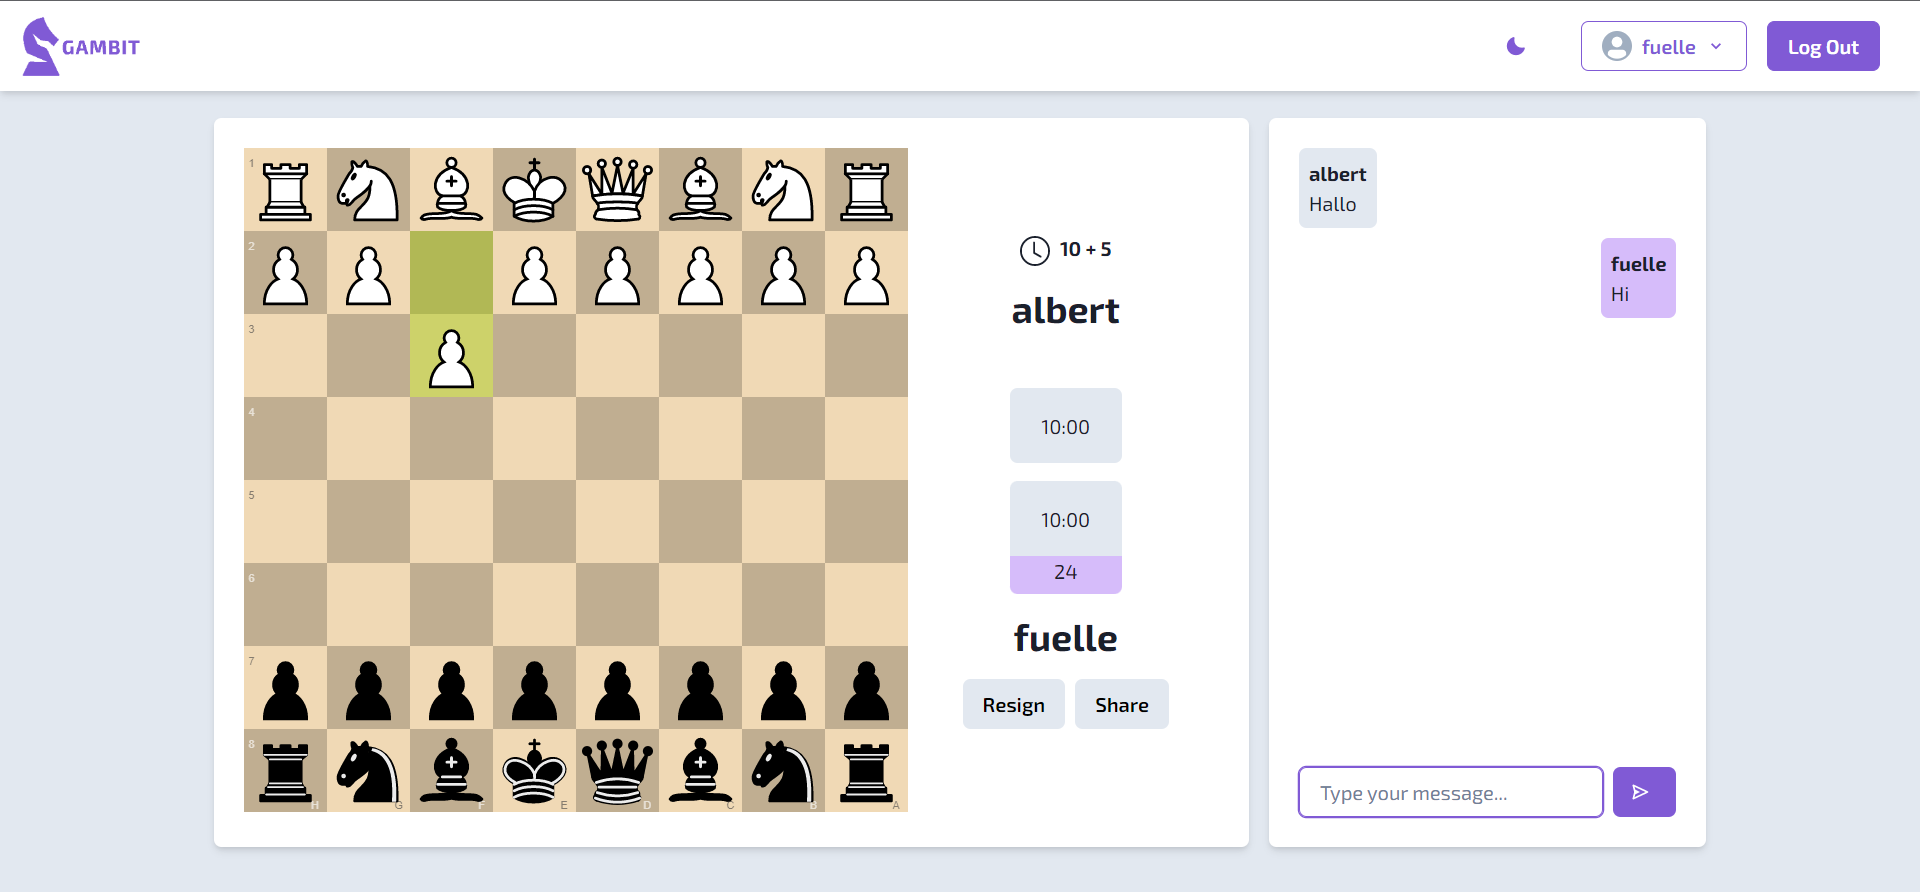
\includegraphics[width=\textwidth]{ChessGame.png}
  \caption{Beispiel einer ChessGame-Komponente} 
  \label{fig:chess-game}
\end{figure}
        
      \begin{figure}[htbp]
      \centering
  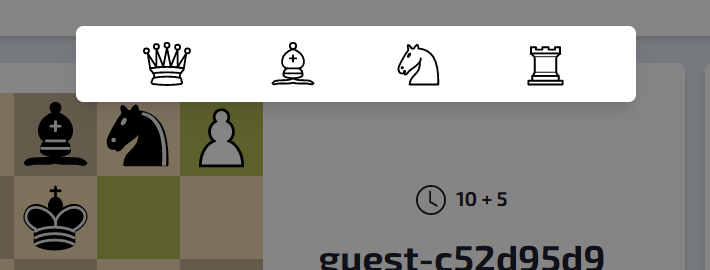
\includegraphics[width=0.7\textwidth]{PromotionModal.png}
  \caption{Das Modal der Komponente PromotionModal}
  \label{fig:PromotionModal}
\end{figure}

    
   
   \subsection{Authentifizierung}
   \label{sec:Autehtifizierung Frontend}
Die Authentifizierung findet in drei Komponenten statt: Dem \textit{UserContext} und den \textit{Login}- und \textit{SignUp}-Komponenten. Die Authentifizierung im Backend, wird in Abschnitt \ref{sec:Authentifizierung Backend} erläutert. Konkrete Einzelheiten und Code-Beispiele werden in Abschnitt \ref{sec:Auth-Impl-Front} vorgestellt.

Der \textit{UserContext} beinhaltet den State \verb|user|, der den Komponenten zur Verfügung gestellt wird.
Nach dem rendern der Komponente wird im \textit{UserContext} eine GET HTTP Anfrage an den Server unter dem Pfad \verb|/auth/login| gesendet. Diese beinhaltet, falls vorhanden, den Cookie mit dem auf dem Server authentifiziert werden kann. Daraufhin sendet der Server die Antwort, ob der Benutzer angemeldet werden konnte oder nicht und wenn ja, dann seinen Benutzernamen.
Dies wird in den \verb|user|-State gesetzt.

Die Authentifizierung der \textit{Login}- und \textit{SignUp}-Komponenten ist simpel gehalten. Mittels Formik und Yup (siehe Abschnitt \ref{sec:weiteres}) werden die Formulare überprüft und gegebenenfalls als POST HTTP Anfrage unter \verb|/auth/signup| oder \verb|/auth/login| an den Server gesendet. Falls es dabei auf dem Server einen Fehler gab, wird die Fehlermeldung angezeigt oder man erhält als Antwort die Benutzerdaten, welche in den \textit{UserContext} gespeichert werden (siehe Abbildungen \ref{fig:SignUp} \& \ref{fig:Login}).
        
        \subsection{Das Schachspiel}
        \label{sec:Schachspiel}
        In diesem Kapitel werde ich näher darauf eingehen wie das Schachspiel im Frontend verwaltet und aktualisiert wird. Die Vorgehensweise im Backend und das Zusammenspiel bei der Gegner Suche befindet sich in Abschnitt \ref{sec:Schach-Backend}.
        
Das Schachspiel und die zugehörigen Schachuhren sind getrennt gehalten um die Modularität und Wartbarkeit zu erhöhen. Die Schachuhren und das Spiel haben jeweils eigene Events die sie empfangen und senden und kommunizieren nur bei der Initialisierung miteinander und sonst nur mit dem Server.
		\subsubsection{Das Starten eines Schachspiels}
		\label{sec:Frontend-Schach-Start}
Um eine Schachpartie zu starten können entweder die Buttons in der Mitte des Bildschirms der \textit{Home}-Komponente (siehe Abbildung \ref{fig:home-logged-in}) oder die Herausforderung zu einer Partie eines Freundes verwendet werden.

Beim klicken auf eines der Zeitkonfigurations-Buttons in der \textit{Home}-Komponente wird das Event \verb|find_game| mit dem aktuellen Benutzerzustand der \textit{UserContext}-Komponente und der Auswahl der Zeitkonfiguration gesendet. Solange man auf einen zufälligen Gegner wartet erscheint ein Lade-Bildschirm, mit einem Button um den Suchvorgang eines Gegners abzubrechen (siehe Abbildung \ref{fig:searching-for-opponent}). Bei solch einem Abbruch wird das Event \verb|leave_queue| mit der Zeitkonfiguration gesendet.

\begin{figure}[h]
\centering
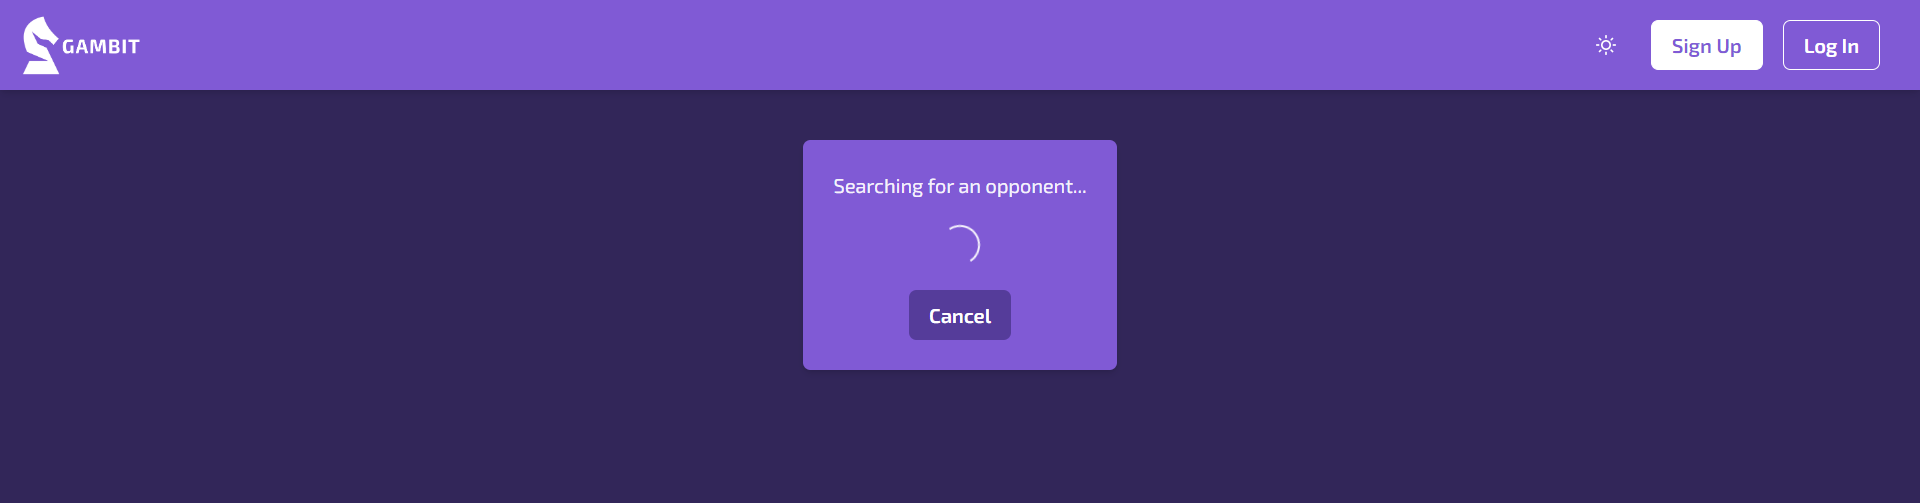
\includegraphics[width=\textwidth]{searching-for-opponent.png}
\caption{Lade-Bildschirm beim Starten eines Spiels mit den Buttons der \textit{Home}-Komponente}
\label{fig:searching-for-opponent}
\end{figure}

Wurde ein Gegner für diese Zeitkonfiguration gefunden, wird in der \textit{Home}-Komponente das Event \verb|joined_game| mit einer ID unter der das Spiel stattfindet (In Zukunft wird die ID eines Schachspiels \textit{roomId} genannt) und gegebenenfalls einen Gast Benutzernamen empfangen und man wird zu dem Pfad \verb|/game/roomId| weitergeleitet, auf dem eine entsprechende \textit{ChessGame}-Komponente das Schachspiel initialisiert.

Wie man einen Freund zu einer Partie herausfordert und was passiert wenn der Freund die Anfrage akzeptiert oder ablehnt wird in Abschnitt \ref{sec:friend-komponente} erläutert, da dies eine Funktion ist, welche in der \textit{Friend}-Komponente stattfindet.

Wenn man selbst eine Anfrage erhält wird dies mittels der \textit{GameReqeust}-Komponente dargestellt (siehe Abbildung \ref{fig:game-request}). Diese besteht aus einer Liste aller gültigen Anfragen zu einer Partie und hat Listener auf die Events \verb|game_request| und \verb|cancel_game_request|. 

Das Event \verb|game_request| empfängt eine Anfrage zu einer Partie mit den Informationen um welche Zeitkonfiguration es sich handelt und wer der Herausforderer ist. Diese wird ganz einfach der Liste hinzugefügt. 

Das Event \verb|cancel_game_request| wird empfangen, sobald der Freund seine Anfrage zurück zieht. Es enthält den Benutzernamen des Spielers, der die Anfrage gesendet hat und diese Anfrage wird aus der Liste der Anfragen entfernt.

Gesendet werden kann das Event \verb|game_request_response| mit den Informationen um welche Anfrage es sich handelt und ob man die Anfrage akzeptiert oder ablehnt.
        \subsubsection{Das Spiel}
        \label{sec:Das-Schachspiel-Front}
Das Schachspiel findet in der Komponente \textit{ChessGame} statt.
Nach dem rendern der Komponente wird das \verb|get_game_data| Event mit der roomId des Spiels und einer Callback Methode gesendet, die die Daten des Spiels beinhaltet, falls dieses existiert. Falls diese Partie nicht im Backend existiert, also keine Daten gesendet werden, wird der Benutzer darauf hingewiesen (siehe Abbildung \ref{fig:game-does-not-exist}).

\begin{figure}[h]
\centering

\includegraphics[width=\textwidth]{game-does-not-exist.png}
\caption{Benachrichtigung, falls kein Spiel unter der roomId gefunden werden konnte}
\label{fig:game-does-not-exist}
\end{figure}

Die Daten die gesendet werden umfassen folgendes:
\begin{itemize}
\item Der Namen des weißen und des schwarzen Spielers.
\item Welcher Zeitmodus gespielt wird (z.B.: 5 + 3, 10 + 5, ...)
\item Die aktuelle Stellung der Partie
\item Die bisherigen Nachrichten im Chat.
\item Die aktuelle Phase des Spiels: Dabei gibt es die vier Möglichkeiten, dass die Startzeit von Schwarz oder Weiß läuft oder dass die reguläre Zeit von Schwarz oder Weiß läuft.
\item Die aktuellen Zeiten der Spieler.
\end{itemize}
Dieses Einholen der Informationen wird für den Fall benötigt, dass die Seite geladen wird, nachdem das Spiel bereits in Gang ist. Außerdem kann dadurch jede Person, die den Link der Partie eingibt oder durch einen Freund dort landet der Partie zuschauen.

Aufgrund der gesendeten Namen der Spieler wird entschieden, ob man ein Zuschauer oder ein Spieler ist.  Dafür werden die Benutzernamen mit dem eigenen Benutzernamen im \textit{UserContext} verglichen. Doch was passiert wenn man eine Partie als unangemeldeter Benutzer spielt und deshalb keinen Benutzernamen im \textit{UserContext} hat?

Bei dem Event \verb|joined_game| (siehe Abschnitt \ref{sec:Frontend-Schach-Start}) wird der Gast-Benutzername des Spielers gesendet und in \verb|location.state| gesetzt\footnote{Quelle: \url{https://github.com/remix-run/history/blob/main/docs/api-reference.md\#locationstate} am 04. Mai 2023}. Dadurch kann in der \textit{ChessGame}-Komponente darauf zugegriffen werden und es kann überprüft werden, ob es sich um einen Spieler oder Zuschauer handelt.


Dem entsprechend wird auch bestimmt wie das Schachbrett, die Namen und die Schachuhren ausgerichtet sind. Ist man Zuschauer wird in chessground definiert, dass man keine Figuren bewegen kann und es gibt kein input Feld für den Chat, sodass man keine Nachrichten abschicken kann. Dies verhindert, dass ein Zuschauer Tipps geben könnte.

Zum Spielen der Partie werden folgende Listener definiert:
\begin{itemize}
\item \verb|opponent_move|: Dient zu Empfangen eines Zugs eines Spielers.
\item \verb|checkmate|: Ein Event welches bei Schachmatt mit dem Benutzernamen des Gewinners empfangen wird.
\item \verb|time_over|: Ist eine Benachrichtigung, dass die Zeit eines Spielers abgelaufen ist.
\item \verb|draw|: Kommuniziert ein Patt der Partie.
\item \verb|resigned|: Signalisiert, dass ein Spieler aufgegeben hat.
\item \verb|cancel_game|: Das Spiel wird aufgrund der abgelaufenen Startzeit abgebrochen.
\end{itemize}
Die Events \verb|checkmate|, \verb|time_over|, \verb|draw|, \verb|resigned| und \verb|cancel_game| beschreiben alle das Ende des Schachspiels. In ihren Listenern wird definiert, dass man keine Figur des Schach Interfaces von chessground mehr bewegen darf und man wird über den Ausgang des Spiels in Form von einem Toast benachrichtigt (siehe Abbildung \ref{fig:resign-toast}).

\begin{figure}[h]
\centering
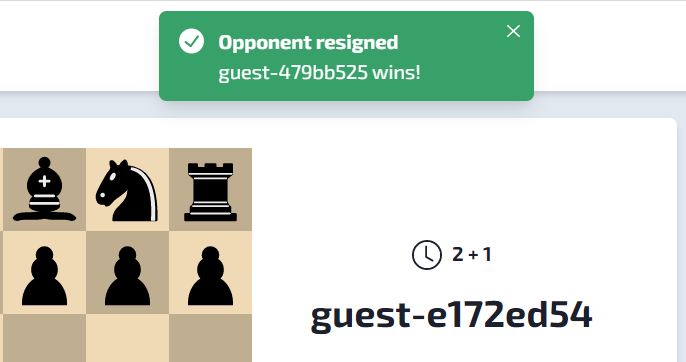
\includegraphics[width=0.5\textwidth]{Toast-resign.png}
\caption{Beispiel eines Toasts, falls der Gegner aufgegeben hat}
\label{fig:resign-toast}
\end{figure}

Der Ablauf beim Empfangen eines neuen Zugs ist im Aktivitätsdiagramm in Abbildung \ref{fig:chess-opponent-move} dargestellt. Die Bauernumwandlung und das en passant müssen separat behandelt werden, da chessground nur das Schach-Interface zur Verfügung stellt und bei diesen beiden Zusatzregeln andere Figuren ersetzt oder entfernt werden, als bei regulären Zügen. Das Aktualisieren möglicher Züge beinhaltet, dass chessground alle möglichen Züge von chess.js übertragen bekommt, welches zur Folge hat, dass bei einem Klick auf eine Figur korrekt angezeigt wird wohin diese Figur ziehen könnte und auch nur auf diese Felder kann diese Figur bewegt werden (siehe Abbildung \ref{fig:chess-game}).

Gesendet werden können die Events: \verb|new_move| zum senden eines Zugs, \verb|resign| zum Aufgeben der Partie und \verb|leave_room|, wenn der Spieler die \textit{ChessGame} Komponente verlässt.
Das \verb|leave_room|-Event ist insofern wichtig, als dass es ermöglicht mehrere Spiele gleichzeitig zu spielen. Wenn der Spieler eine Partie verlässt und eine zweite Partie startet und weiterhin die Events des ersten Spiels empfängt kann es zu Problemen kommen, da die Listener der neuen Partie die Events der alten Partie empfangen. Durch das Verlassen des Raums wird gewährleistet, dass ein Spieler immer nur die Events zu dem Spiel empfängt, auf dem er sich gerade befindet.

Ein Aktivitätsdiagramm des Sendens eines Zugs befindet sich in Abbildung \ref{fig:chess-move}. Genau wie bei dem Empfangen eines Zugs wird auch beim Senden zwischen Bauernumwandlung und En Passant unterschieden. Der einzige Unterschied ist, dass bei der Bauernumwandlung nach dem Setzen des Zugs noch mittels der  \textit{PromotionModal}-Komponente ausgewählt werden muss, in welche Figur sich der Bauer umwandeln soll, bevor der Zug gesendet wird.

Das Event zum Aufgeben wird nach dem klicken des \glqq resign\grqq{ }Buttons gesendet.


      \begin{figure}[h]
      \centering
  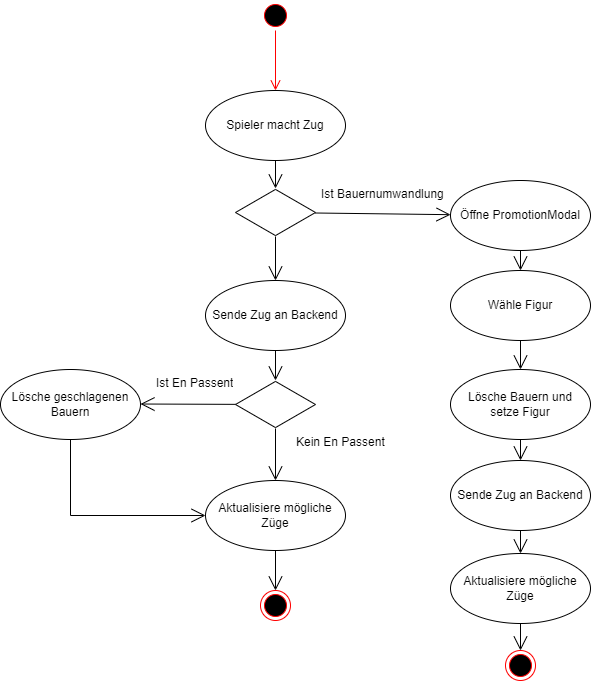
\includegraphics[width=0.8\textwidth]{Interaktion Schach Zug.png}
  \caption{Aktivitätsdiagramm eines Schachzugs}
  \label{fig:chess-move}
\end{figure}

      \begin{figure}[h]
      \centering
  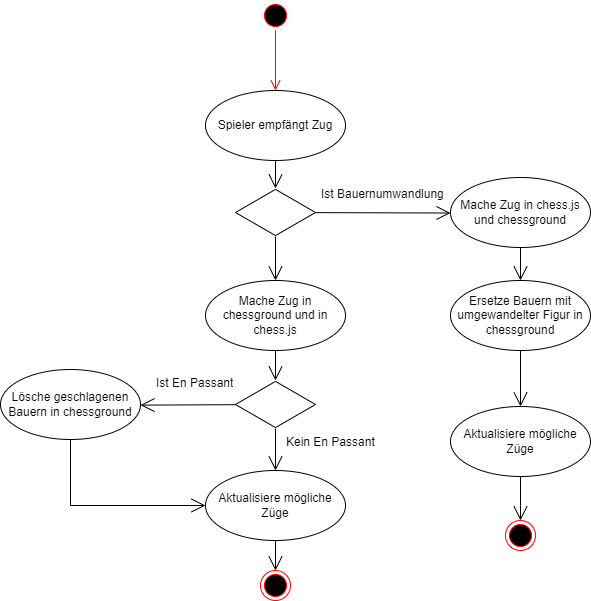
\includegraphics[width=0.8\textwidth]{Interaktion Schach Zug empfangen.png}
  \caption{Aktivitätsdiagramm eines empfangenen Schachzugs}
  \label{fig:chess-opponent-move}
\end{figure}

        \subsubsection{Die Uhr}
        \label{sec:Frontend-Uhr}
Die \textit{ChessClock} Komponente bekommt von \textit{ChessGame} als Props die aktuelle Phase der Partie, die jeweiligen aktuellen Zeiten und die Ausrichtung, welche Zeit oben bzw. unten gezeigt werden soll. Neben der regulären Schach Zeit gibt es noch eine Startzeit, welche während des ersten Zugs jedes Spielers abläuft, um zu gewährleisten, dass das Spiel auch erst wirklich startet sobald beide Spieler bereit sind. Läuft die Startzeit ab wird das Spiel abgebrochen (siehe Abschnitt \ref{sec:schach-theorie}). Diese Startzeit ist die lila eingefärbte Zeit in Abbildung \ref{fig:chess-game}.

Die Komponente sendet keine Events, sondern hört nur auf die folgenden:
\begin{itemize}
\item \verb|updated_time|: Dieses Event wird vom Backend gesendet, sobald ein Zug gemacht wurde und enthält die aktuellen Zeiten der Spieler nach dem Zug und welcher Spieler jetzt am Zug ist. Dementsprechend werden die Zeiten aktualisiert und die Uhr des Spielers, welcher jetzt dran ist wird gestartet.
\item \verb|stop_starting_time_white|: Stoppt die Startzeit des weißen Spielers und startet die Startzeit des schwarzen Spielers.
\item \verb|stop_starting_time_black|: Stoppt die Startzeit des schwarzen Spielers und lässt die reguläre Zeit des weißen Spielers beginnen.
\item \verb|stop_clocks|: Wird bei Beendung des Spiels empfangen und stoppt die aktive Uhr.
\end{itemize}

\subsubsection{Der Chat}
Die \textit{Chat}-Komponente bekommt als props alle bisher gesendeten Nachrichten, die roomId unter der das Spiel stattfindet, die Information ob es sich um einen Zuschauer handelt und gegebenenfalls den Gastnamen, falls es sich um einen nicht angemeldeten Benutzer handelt. Handelt es sich um einen Zuschauer wird das Input-Feld der Komponente nicht angezeigt, um keine Nachrichten schreiben zu können. Die Komponente ist relativ simpel und sendet das Event \verb|send_message|, um eine Nachricht zu senden und empfängt eine Nachricht mit dem \verb|message| Event. Eine Nachricht beinhaltet immer den Namen des Versenders, die Nachricht als String und die roomId des Spiels. Je nachdem ob der Versender der Nachricht mit dem eigenen Namen übereinstimmt wird die Nachricht unterschiedlich ausgerichtet und eingefärbt (siehe Abbildung \ref{fig:chess-game}).

\subsection{Verwaltung von Freunden}
\label{sec:Friends}
Die Verwaltung und Darstellung (siehe Abbildung \ref{fig:home-logged-in}) von Freunden und Freundschaftsanfragen obliegt der \textit{FriendList}-Komponente. Diese beinhaltet die Unterkomponenten \textit{Friend}, \textit{FriendReqeust} und \textit{AddFriendModal}.

\subsubsection{\textit{FriendList}-Komponente}
\label{sec:FriendList}
\textit{FriendList} verwendet zwei States in Form von Arrays: \verb|friends| und \verb|friendRequests|. Je ein Element dieser Listen wird durch eine \textit{Friend}-, beziehungsweise \textit{FriendRequest}-Komponente dargestellt und verwaltet. Dabei werden die Freunde je nachdem ob sie online sind oder nicht sortiert. \textit{FriendList} hört dabei auf die folgenden Events: 
\begin{itemize}
\item \textbf{friend\_request\_accepted:} Enthält Daten eines neuen Freundes, welcher deine Freundschaftsanfrage angenommen hat. Dieser wird der Freundesliste hinzugefügt.
\item \textbf{friend\_request:} Eingang einer neuen Freundschaftsanfrage. Wird der Liste der Freundschaftsanfragen hinzugefügt.
\item \textbf{connected:} Dieses Event wird empfangen, falls ein Freund offline, beziehungsweise online geht. Der betreffende Freundes-Eintrag in der Freundesliste wird aktualisiert.
\end{itemize}

Zum Holen der Listen werden die zwei Events \verb|get_friends| und \verb|get_friend_requests| jedes Mal gesendet, wenn auf die \verb|Home|-Komponente navigiert wird. Diese beiden Events empfangen mittels Callback-Funktionen alle Daten über die Freunde und Freundschaftsanfragen. Dies ist nötig, damit, falls beispielsweise nach einer Schachpartie wieder auf die \textit{Home}-Komponente navigiert wird, die Daten der Freunde aktualisiert werden.

\subsubsection{\textit{Friend}-Komponente}
\label{sec:friend-komponente}
Diese Komponente stellt einen Freund dar. Es kriegt als props den Benutzernamen, die aktiven Spiele und seinen online Status übergeben. Sie hat zwei Grundlegende Funktionen: Das Zuschauen einer Partie eines Freundes und das Herausfordern zu einer Partie. Beim Herausfordern eines Freundes sind genau die gleichen Schachuhren möglich, wie bei der Suche eines zufälligen Gegners und das Zuschauen ist aufgebaut wie bei der \textit{ActiveGames}-Komponente. (siehe Abbildung \ref{fig:Freunde-zuschauen-herausfordern})

Diese beiden Funktionen sind nur verfügbar, falls der Freund gerade online ist, welches über einen grünen Punkt ersichtlich ist und zum Zuschauen benötigt der Freund trivialerweise mindestens ein aktives Spiel.

Die Komponente hat zwei Eventlistener: \verb|game_request_accepted| und \linebreak \verb|game_request_denied|, welche einen Toast darstellen und den Spieler gegebenenfalls zu dem Spiel navigieren. 

Senden tut die Komponente zwei Events: \verb|send_game_request| und \verb|cancel_game_request|. Wurde eine Herausforderung zu einer Partie versendet, erscheint ein Lade-Bildschirm, bis der Spieler die Anfrage angenommen, beziehungsweise abgelehnt hat. Entscheidet sich der Spieler davor doch nicht mehr gegen den Freund zu spielen, kann er auf den \glqq Cancel\grqq{ }Button klicken und die Spielanfrage wird zurückgenommen.

\begin{figure}[h]
\centering
  \begin{subfigure}[c]{0.35\textwidth}
  \centering
  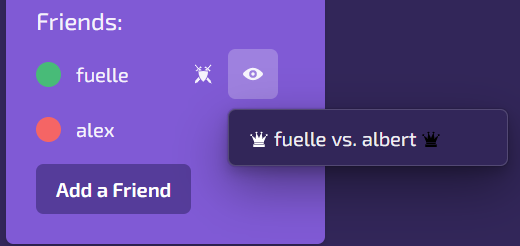
\includegraphics[width=\linewidth]{activeGames-friends.png}
  \caption{Aktive Partien eines Freundes}
  \label{fig:activeGames-friends}
  \end{subfigure}
  \hfill
  \begin{subfigure}[c]{0.3\textwidth}
  \centering
    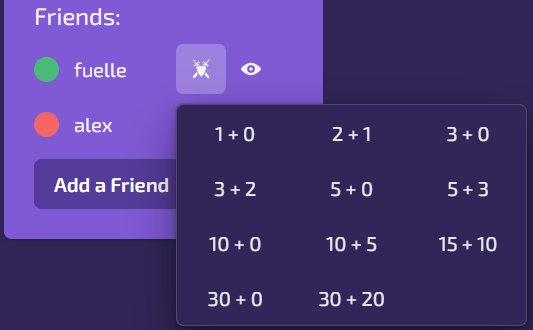
\includegraphics[width=\linewidth]{Spiel-herausfordern.png}
  \caption{Das Herausfordern eines Freundes}
  \label{fig:spiel-herausfordern}
  \end{subfigure}
  \hfill
 \begin{subfigure}[c]{0.3\textwidth}
  \centering
    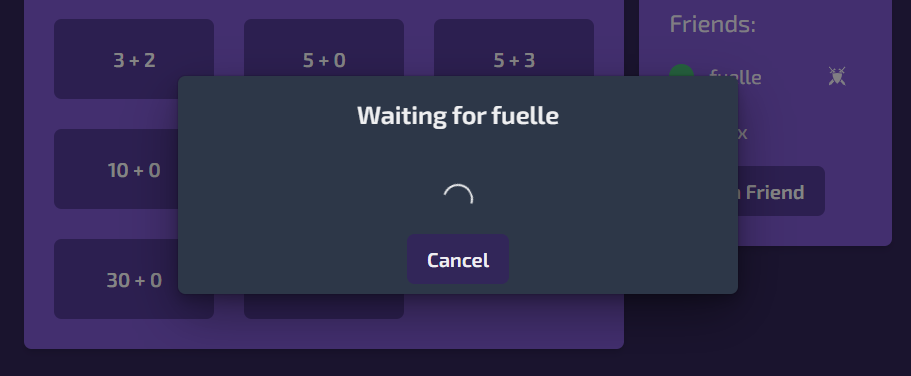
\includegraphics[width=\linewidth]{waiting-for-friend.png}
  \caption{Warte auf Freund Modal}
  \label{fig:waiting-for-friend}
  \end{subfigure}
  \caption{Das Herausfordern und Zuschauen bei Freunden}
  \label{fig:Freunde-zuschauen-herausfordern}
 
\end{figure}


\subsubsection{\textit{FriendRequest}-Komponente}
Die \textit{FriendRequest}-Komponente stellt eine Freundschaftsanfrage dar und erhält ebenfalls seine Daten von der \textit{FriendList}-Komponente, wozu auch die Funktionen \verb|setFriends| und \verb|setFriendRequest| zählen, um die Listen der \textit{FriendList}-Komponente zu ändern.
Es hört auf keine Events, sendet allerdings zwei Events: \verb|accept_friend_request| und \verb|decline_friend_request|. Die Behandlung dieser Events im Backend wird in Abschnitt \ref{sec:accept-friend-request} erläutert. War das Akzeptieren, beziehungsweise das Ablehnen der Anfrage erfolgreich wird die Freundschaftsanfrage aus der Liste gelöscht und zusätzlich wird gegebenenfalls der neue Freund der Freundesliste hinzugefügt. Dieser wird mittels Callback Funktion empfangen.

\subsubsection{\textit{AddFriendModal}-Komponente}
Diese Komponente besteht aus einem Button und einem Modal, das sich öffnet, falls man den Button anklickt. In diesem Modal kann man einen Benutzernamen angeben, an den die Freundschaftsanfrage verschickt werden soll. Das Versenden einer Freundschaftsanfrage wird mittels des \verb|send_friend_request|-Events behandelt. Es beinhaltet eine Callback-Funktion, welche entgegennimmt, ob die Versendung erfolgreich war und wenn nicht, dann eine Fehlermeldung, warum es nicht möglich war die Freundschaftsanfrage zu versenden (siehe Abbildung \ref{fig:AddFriendModal}). Wie das Backend eine neue Freundschaftsanfrage behandelt wird in Abschnitt \ref{sec:hinzufügen-von-Freunden} erläutert.

\begin{figure}[h]
\centering
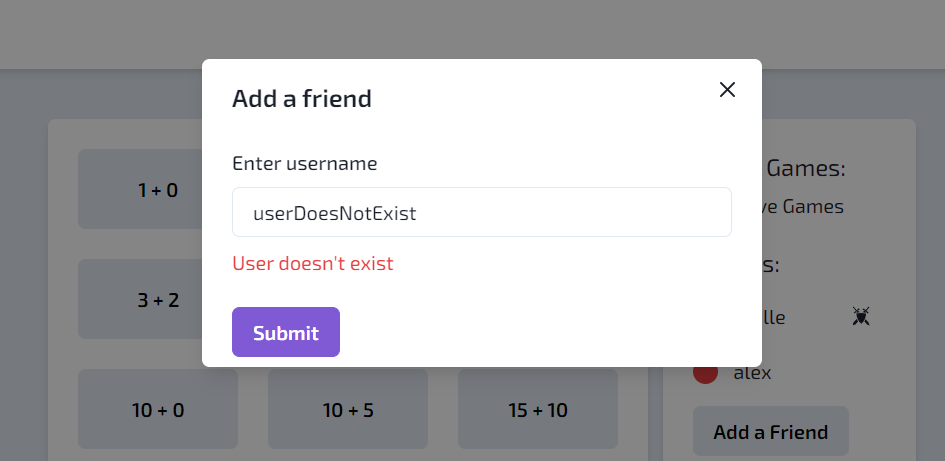
\includegraphics[width=0.7\textwidth]{AddFriendModal.png}
\caption{Das Modal der \textit{AddFriendModal}-Komponente mit Fehlermeldung}
\label{fig:AddFriendModal}
\end{figure}

\subsection{Anzeigen und navigieren zu aktiven Partien}
Falls man eine aktive Schachpartie spielt und aus Versehen den Browser schließt, auf die Startseite navigiert oder ähnliches gäbe es keine Möglichkeit auf das Spiel zurück zu kehren, es sei denn man hat den Link oder die roomId des Spiels gespeichert. Um es möglich zu machen auf aktive Spiele schnell wieder zurück zu kehren, ohne die roomId der Partie zu kennen, gibt es die Unterkomponente \textit{ActiveGames} in der \textit{Home}-Komponente (siehe Abbildung \ref{fig:home-logged-in}). Diese Komponente macht es möglich zu verfolgen welche offenen Spiele man gegen wen in welcher Farbe hat und man kann leicht wieder zu diesen Spielen navigieren, indem man auf den Button klickt.

Es sendet das Event \verb|get_active_games|, welches mit einer Callback Funktion  eine Liste aller aktiven Spiele empfängt. Dieses Event wird, wie bei dem Event \verb|get_friends| von der \textit{FriendList}-Komponente (siehe Kapitel \ref{sec:FriendList}), jedes mal gesendet, wenn auf die \textit{Home}-Komponente navigiert wird, um die Liste der aktiven Spiele zu aktualisieren.
Ist die Liste leer, wird nur \glqq No acitve Games\grqq{ } angezeigt. Ansonsten wird jedes aktive Spiel der Liste mit einem Button dargestellt, auf deren klick man zu dem Spiel navigiert wird.

        \section{Backend-Architektur}
Das Backend basiert auf Node.js mit dem Express Framework. Des weiteren werden als Schnittstellen mit dem Frontend eine Web-API für HTTP Anfragen und ein Socket.io Server bereitgestellt. Das Backend kommuniziert mit zwei Datenbanken: einer PostgreSQL Datenbank für die Benutzerverwaltung und eine Redis Datenbank für häufig aktualisierte und angefragte Daten.

Die Ordnerstruktur des Backends (Abbildung \ref{fig:backend_dirtree}) ist auf dieser Weise aufgebaut:

\begin{itemize}
\item \textbf{auth:} Dieser Ordner beschäftigt sich sowohl mit der Schnittstelle der Web-API-Kommunikation mit dem Frontend, als auch deren Behandlung und dem Austausch mit der PostgreSQL Datenbank. Diese Schnittstellen dienen bloß der Anmeldung und Registrierung eines Benutzers.
\item \textbf{chess:} Stellt ein chess.js Schachspiel und die serverseitige Schachuhr zur Verfügung.
\item \textbf{redis:} Dient als Schnittstelle und Verwalter von Operationen auf der redis Datenbank.
\item \textbf{sockets:} Stellt Middleware für die Verbindungsherstellung und Listener für die Kommunikation zwischen Frontend und Backend bereit.
\item \textbf{index.js:} Initialisiert den Server mit seinen Schnittstellen.
\end{itemize}

\begin{figure}[h]
\centering

\begin{minipage}{0.5\textwidth}
\dirtree{%
.1 server/.
.2 src/.
.3 auth/ .
.4 authController.js.
.4 database.js.
.4 rateLimiter.js.
.4 validateForm.js.
.3 chess/.
.4 Chess.mjs.
.4 ServerChessClock.js.
.3 redis/.
.4 redis.js.
.4 redisController.js.
.3 routers/.
.4 authRouter.js.
.3 sockets/.
.4 socketChessController.js.
.4 socketController.js.
.4 socketMiddleware.js.
.2 .env.
.2 index.js.
.2 package.json.
}
\end{minipage}
\caption{Ordnerstruktur des Backends}
\label{fig:backend_dirtree}

\end{figure}


\subsection{Authentifizierung}
\label{sec:Authentifizierung Backend}
Die Authentifizierung eines Benutzers läuft über HTTP Anfragen an die Web-API und einer PostgreSQL Datenbank.
Nachdem die erste Authentifizierung stattgefunden hat wird die Socket.io Verbindung des Clients hergestellt, in der die Socket Verbindung nochmals Authentifiziert wird.
Es gibt drei verschiedene Möglichkeiten wie ein Benutzer authentifiziert werden kann: Durch das Anmelden, durch das Registrieren oder durch das Lesen des Cookies.

Die Authentifizierung im Frontend wird in Abschnitt \ref{sec:Autehtifizierung Frontend} erläutert.

\subsubsection{Authentifizierung mit der Web-API und PostgreSQL}
Das Anmelden und Registrieren mittels Formular läuft über eine POST Anfrage des Clients an den Pfad \verb|/auth/login|, beziehungsweise \verb|/auth/signup|, die die angegebenen Formulardaten beinhaltet. Bei der Verarbeitung der Anfrage werden mittels des Express Routings verschiedene Middlewares verwendet.

Bei jeder Anfrage an die API stellt eine Middleware sicher, dass die Anzahl der Anfragen über eine IP-Adresse in einer bestimmten Zeit begrenzt wird. Dies verhindert sogenannte Denial-of-Service (kurz: DoS) Attacken\footnote{Quelle: \url{https://www.bsi.bund.de/DE/Themen/Verbraucherinnen-und-Verbraucher/Cyber-Sicherheitslage/Methoden-der-Cyber-Kriminalitaet/DoS-Denial-of-Service/dos-denial-of-service_node.html} am 27. April 2023}, bei denen probiert wird den Server mit so vielen Anfragen zu belasten, dass dieser außer Betrieb gesetzt wird.

Anschließend überprüft eine Middleware, ob die angegebenen Daten mit dem Schema übereinstimmen. 

Treten bei diesen beiden Middlewares keine Fehler auf wird beim Anmelden überprüft, ob dieser Benutzer in der Datenbank existiert und es wird mittels bcrypt kontrolliert, ob die Passwörter übereinstimmen. Ist dies der Fall, wird ein JWT-Token mit den Benutzerinformationen erstellt und als Cookie in den Browser des Clients gesetzt. Des Weiteren wird dem Benutzer geantwortet, dass die Anmeldung erfolgreich war mit der Übermittlung des Benutzernamens.

Beim Registrieren wird überprüft, ob bereits ein Nutzer mit dem Benutzernamen oder E-Mail existiert und anschließend wird ein neuer Tupel in der PostgreSQL Datenbank erstellt. Das Passwort wird dafür mittels bcrypt verschlüsselt und es wird eine individuelle \verb|userid| generiert. Diese dient zur Socket.io-Kommunikation.

Bei dem ersten Aufruf der Seite vom Client wird eine GET Anfrage an \verb|/auth/login| gestellt. Bei dieser wird ebenfalls die Middleware gegen DoS-Attacken verwendet und anschließend wird überprüft, ob er einen gültigen JWT-Token im Cookie hat und ihm wird dem entsprechend geantwortet. Das Setzen des Tokens im Cookie hat den Vorteil, dass bei einem neuen Aufruf der Seite, solange der Cookie noch gültig ist, der Benutzer automatisch angemeldet wird, ohne seine Anmeldedaten nochmals einzugeben.

Anschließend stellt der Client eine Socket.io Verbindung her.

\subsubsection{Authentifizierung und anschließende Middleware mit Socket.io}
\label{sec:socketauth}
Bei der Verbindungsherstellung des Clients mit dem Socket.io Server durchläuft die Socket verschiedene Middlewares.

Die erste Middleware Authentifiziert die Socket des Benutzers. Sie liest aus dem Cookie, der auch in der Socket mitgesendet wird, den JWT-Token, falls dieser existiert. Die Daten die in dem Token kodiert sind werden dann in der Socket als Attribute gesetzt, sodass anschließend immer mittels \verb|socket.user| darauf zugegriffen werden kann.

Wenn der Benutzer keinen gültigen JWT-Token hat, werden trotzdem alle Middlewares ohne Fehler durchlaufen. Dies liegt daran, dass bei einem fehlgeschlagenen Middleware-Prozess die Socket.io-Verbindung abgelehnt werden würde. Es soll allerdings auch das Spielen einer Schachpartie als Gast möglich sein.

In der zweiten Middleware tritt die Socket der \verb|userid| des Benutzers als Raum bei und wird sowohl in der Redis Datenbank unter \verb|user:username| (siehe Kapitel \ref{sec:redis-data}) , als auch bei Freunden mittels des Events \verb|connected|, als online vermerkt.
Der Beitritt der eigenen \verb|userid| dient als Kommunikationsschnittstelle. So können Event immer diese \verb|userid| verwenden um ein Event an diesen Benutzer zu senden.

Beim Schließen der Anwendung oder Abmelden des Benutzers wird dementsprechend in Redis \verb|connected| auf \verb|false| gesetzt und die Freunde werden mit dem Event \verb|connected| darüber in Kenntnis gesetzt, dass der Benutzer nicht mehr online ist.

Als letzte Middleware werden alle nötigen Listener sowohl für das Schachspiel, als auch für sonstige Funktionen initialisiert.
\subsection{Das Schachspiel}
\label{sec:Schach-Backend}
In diesem Abschnitt werden die Prozesse beim Suchen eines Gegners, der Initialisierung des Schachspiels, der Ausführung neuer Züge sowie dem Senden und Empfangen von Nachrichten im Chat detailliert beschrieben.
\subsubsection{Finden eines Gegners}
\label{sec:find_game}
Es gibt 3 verschiedene Möglichkeiten ein Schachspiel zu starten: Ein unangemeldeter Benutzer sucht einen zufälligen Gegner, ein angemeldeter Benutzer sucht einen zufälligen Gegner oder ein angemeldeter Benutzer spielt gegen einen Freund.

Das Suchen eines Spiels mit zufälligem Gegner wird mittels des Events \verb|find_game| mit den Benutzerdaten und der gewählten Zeitkonfiguration vom Frontend gesendet. Ein Sequenzdiagramm des Initialisieren eines Spiels mit zufälligem Gegner befindet sich in Abbildung \ref{fig:sequence_chess_start}. Dies beinhaltet folgende Schritte:
     
\begin{figure}[!htbp]
  \centering
  
 
\begin{adjustbox}{height=\textheight}
  \begin{sequencediagram}
    \newinst{clientA}{Client A}
    \newinst[2]{clientB}{Client B}
    \newthread{server}{Server}
    \tikzstyle {inststyle}+=[rounded corners=3mm]
    \newinst[3]{redis}{Redis DB}
    
    \begin{messcall}{clientA}{find\_game}{server}
    \begin{call}{server}{getPlayerInQueue}{redis}{player}
    \end{call}
    
    \begin{sdblock}{Kein Spieler in der Warteschlange}{}
    	\begin{messcall}{server}{addPlayerInQueue}{redis}{}
    	\end{messcall}
    	\end{sdblock}
    	
    	\begin{messcall}{clientB}{find\_game}{server}{}
    	\end{messcall}
    	
    \begin{call}{server}{getPlayerInQueue}{redis}{player}
    \end{call}
    	
    	\begin{sdblock}{Spieler in Warteschlange}{}
    \begin{callself}{server}{createChessGame}{roomId}
    \end{callself}
    \postlevel
    	\begin{messcall}{server}{initializeGame}{redis}
    	\end{messcall}
    	\prelevel
    	\begin{messcall}{server}{joined\_game, roomId}{clientA}{}
    	\prelevel\prelevel
    	\mess{clientA}{navigiere zu /game/roomId}{clientA}
    	\postlevel\postlevel
    	\begin{call}{clientA}{get\_game\_data, roomId}{server}{gameData}
    	\begin{call}{server}{Hole Daten des Spiels}{redis}{gameData}
    	\end{call}
    	\end{call}
    	\end{messcall}
    	\prelevel
    	\begin{messcall}{server}{}{clientB}{}
    	\begin{call}{clientB}{}{server}{}
    	\begin{call}{server}{}{redis}{}
    	\end{call}
    	\end{call}
    	\end{messcall}
    	\end{sdblock}
    \end{messcall}
    
    
    
  \end{sequencediagram}
  \end{adjustbox}
  
  \caption{Sequenzdiagramm des Schachspielstartprozesses mit unbekanntem Gegner}
  \label{fig:sequence_chess_start}
\end{figure}


\begin{itemize}
\item Das Event \verb|find_game| mit der Zeitkonfiguration und Benutzerdaten wird gesendet (siehe Abschnitt \ref{sec:Frontend-Schach-Start}).
\item Falls der Benutzer nicht angemeldet ist, wird ihm  ein zufälliger Benutzername für dieses Schachspiel zugewiesen, der mit \glqq guest-\grqq{ }startet. Seine \verb|userid| wird als seine Socket ID festgelegt.
\item Daraufhin wird im Server ein Spieler aus der entsprechenden Warteschlange aus Redis genommen (siehe Abschnitt \ref{sec:Warteschlange}).
\item Falls dabei kein Spieler entnommen werden konnte, wird der Benutzer selbst in die Liste geschrieben und wartet bis er von einem anderen Benutzer aus der Liste genommen wird.
\item Falls ein Spieler aus der Liste entnommen werden konnte, wird das Spiel mit einer roomId als Identifikator initialisiert und in Redis gespeichert. Dabei wird auch ein ServerChessClock Objekt kreiert und in einem Array der socketChessListeners Datei gespeichert.
\item An die beiden Spieler wird das Event \verb|joined_game| mit der roomId und gegebenenfalls dem Gast-Benutzernamen gesendet, woraufhin sie zu dem Pfad \verb|/game/roomId| navigieren, auf der sich die \textit{ChessGame}-Komponente befindet.
\item Die \textit{ChessGame}-Komponente sendet das \verb|get_game_data| Event. Daraufhin wird der aktuelle Zustands der Partie aus Redis geholt und an das Frontend zurück gesendet. Ein Ablauf was im Frontend bei einer Schachpartie passiert befindet sich im Abschnitt \ref{sec:Schachspiel}.
\end{itemize}

Falls es sich um eine Partie handelt, die aus einer Herausforderung eines Freundes resultiert, wird natürlich in keine Warteschlange nach einem Gegner gesucht, anstatt dessen wird mit den Events \verb|send_game_request|, \verb|game_request| und \verb|game_request_response| (siehe Abschnitte \ref{sec:Frontend-Schach-Start}) die Anfrage versendet und beantwortet. Anschließend wird das Spiel initialisiert und an die beiden Spieler das Event \verb|game_request_accepted| mit der roomId gesendet (für Frontend-Informationen zu diesen Events siehe Kapitel \ref{sec:friend-komponente} \& \ref{sec:Frontend-Schach-Start}).

Die Implementierungsdetails, wie ein Schachspiel auf dem Server mittels der Methoden \verb|createChessGame| und \verb|initializeGame| initialisiert und die Informationen des Schachspiels an das Frontend gesendet werden, sind in Kapitel \ref{sec:Schach-Backend-impl} ausführlich beschrieben.

\subsubsection{ServerChessClock}
Die Klasse ServerChessClock definiert einzelne Schachuhr Objekte, welche die Startzeiten und die regulären Zeiten einer Schachpartie verwalten.

socketChessController und ServerChessClock kommunizieren mittels Funktionen und Events miteinander, wobei Events genutzt werden um laufende Uhren anzuhalten und zu kommunizieren, dass eine Startzeit oder eine reguläre Schachuhr abgelaufen ist, während die Funktionsaufrufe von ServerChessClock dazu dienen eine bestimmte Zeit zu starten.

Die Funktionsweise und Beispielcode der serverseitigen Schachuhr werden in Kapitel \ref{sec:Uhr-Backend-impl} erläutert.

\subsubsection{Neuer Zug einer Schachpartie}
\label{sec:Zug-Backend}
Ein Aktivitätsdiagramm zur Behandlung eines neuen Zugs im Backend ist in Abbildung \ref{fig:Zug-Backend} zu finden. 


Sobald ein neuer Zug eines Spielers ankommt wird zunächst die bisherige PGN-Notation des Spiels aus Redis und das ServerChessClock Objekt aus dem Array geholt. Es wird ein neues chess.js Objekt kreiert, welches das aktuelle PGN importiert und anschließend den neuen Zug macht. Daraufhin wird der Zug in die roomId gebroadcastet. Das bedeutet, es wird an alle Sockets im Raum gesendet, außer von dem Sender, da dieser ja bereits den Zug gemacht hat. Die veraltete PGN-Notation des Spiels wird nun mit der neuen Notation in Redis überschieben.

Anschließend wird überprüft ob es sich um ein Schachmatt oder ein Patt handelt, falls ja werden die Uhren der ServerChessClock angehalten, das Frontend wird über den Ausgang informiert und das Spiel wird beendet (siehe Abschnitt \ref{sec:Schach-Ende}). 

Falls dies nicht der Fall ist wird die Zeit des jetzigen Spielers gestoppt und falls es eine reguläre Zeit ist, wird das Inkrement auf die Zeit gerechnet, die Zeit des anderen Spielers fängt an zu laufen und die aktualisierten Zeiten werden an das Frontend gesendet.

Handelt es sich um die ersten zwei Züge, in denen die Startzeit und nicht die reguläre Zeit der Spieler läuft werden diese gesondert betrachtet und entweder die Startzeit von Schwarz beginnt zu laufen oder die reguläre Zeit von Weiß fängt an zu laufen. Dies wird auch mit entsprechenden Events dem Frontend mitgeteilt.

\begin{figure}[h!]
\centering
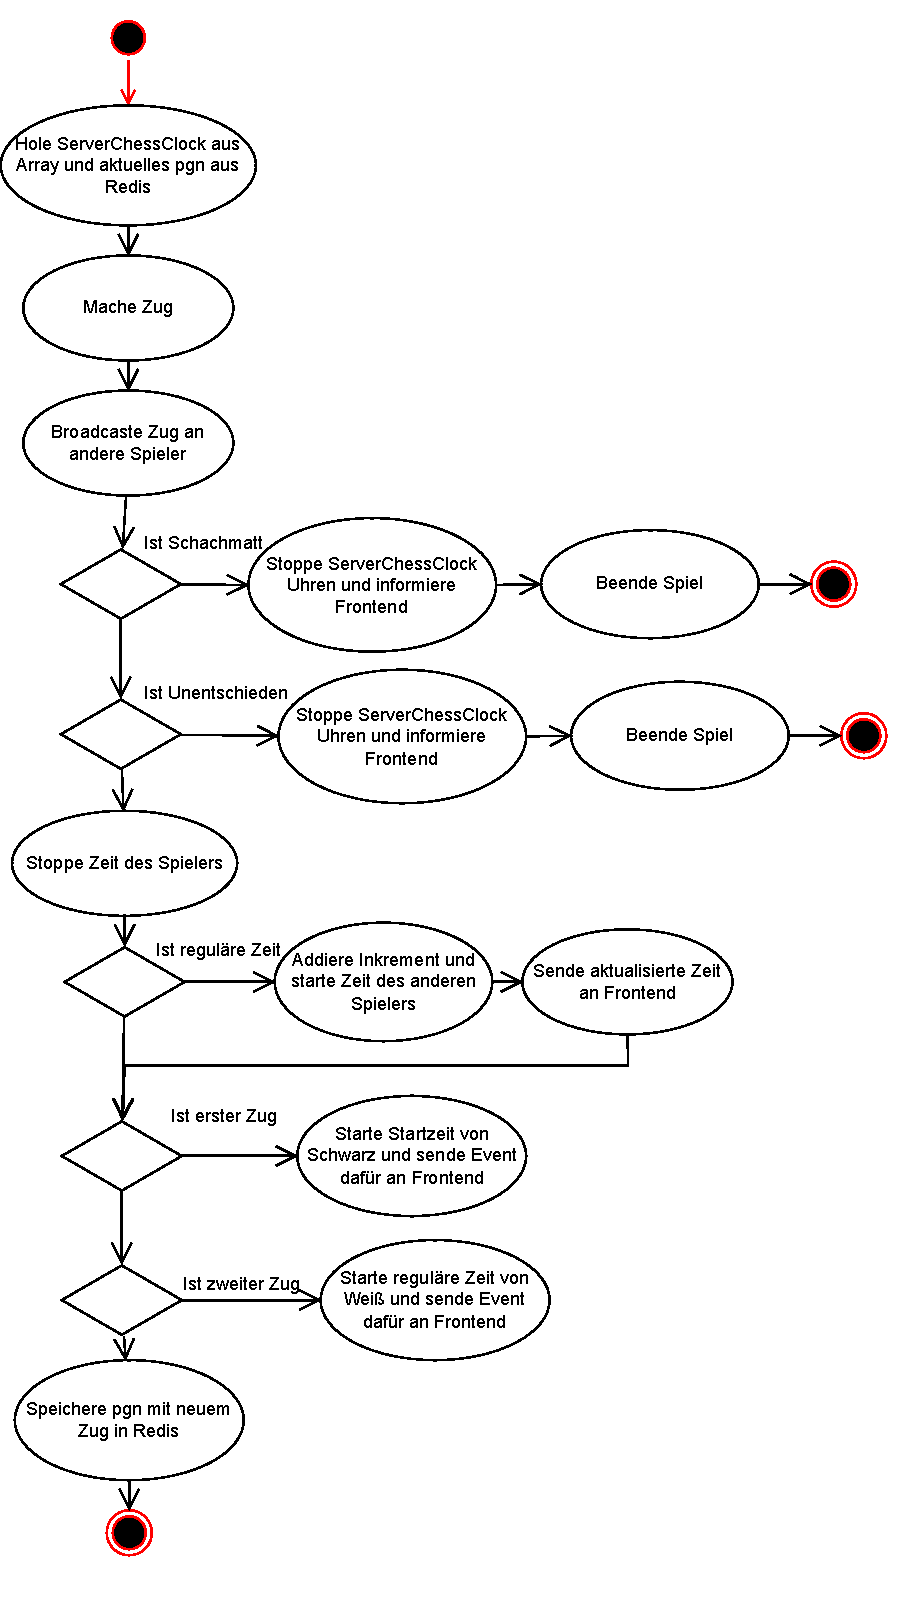
\includegraphics[width=\textwidth]{Neuer Zug Backend.pdf}
\caption{Aktivitätsdiagramm zur Behandlung eines neuen Zugs im Backend}
\label{fig:Zug-Backend}
\end{figure}

\subsubsection{Ende einer Schachpartie}
\label{sec:Schach-Ende}
Das Ende einer Schachpartie kann durch folgende Situationen stattfinden:
Schachmatt, Patt, Startzeit ist abgelaufen, eine reguläre Zeit ist abgelaufen oder ein Spieler hat aufgegeben.

Auf Schachmatt und Patt wird bei neuen Zügen geachtet und an das Frontend gesendet. Wenn das Ende der Partie auf die Schachuhren zurückzuführen ist, wird ein Event von ServerChessClock in socketChessController empfangen und an die Sockets im Raum weitergeleitet. 

Bei einer Aufgabe empfängt das Backend das event \verb|resign| mit der Farbe welche aufgibt und der roomId und leitet dies entsprechend weiter.

Bei jedem dieser Ausgänge einer Partie geschieht noch folgendes:

Das ServerChessClock Objekt wird aus dem Array in socketChessController gelöscht.

Die Benutzernamen werden aus dem Redis Eintrag \verb|game:roomId| geholt und falls es sich um angemeldete Benutzer handelt wird das entsprechende Spiel aus der \verb|activeGames| Liste von \verb|user:username| gelöscht. Anschließend wird der Eintrag \verb|game:roomId| gelöscht.

Somit wird kein Speicher mehr von alten Spielen belegt.

\subsubsection{Chat}
Der Listener auf das Event \verb|send_message| empfängt und verwaltet die neue Nachricht, die ein Spieler gesendet hat. Die Informationen Benutzernamen, roomId und die Nachricht werden dabei empfangen und weitergeleitet.

Dabei passieren zwei Prozesse:
\begin{itemize}
\item Die Nachricht wird in Redis gespeichert. Dafür werden alle alte Nachrichten des Spiels aus \verb|game:roomId| geholt, die neue Nachricht angehängt und anschließend wieder dort gespeichert.
\item Die Nachricht wird an alle im Raum mittels des Events \verb|message| gesendet.
\end{itemize}

\subsection{Verwaltung von Freunden}
\label{sec:hinzufügen-von-Freunden}
In den Aktivitätsdiagrammen in Abbildung \ref{fig:Freunde-backend} ist der Ablauf des Versendens und des Akzeptierens einer Freundschaftsanfrage abgebildet.
Die verschiedenen Datentypen der Speicherung in Redis befindet sich in Abschnitt \ref{sec:redis-data}.

Beispiel Codeausschnitte und Implementierungsdetails über die Verwaltung von Freunden im Backend befindet sich in Kapitel \ref{sec:Freunde-impl}.

\subsubsection{Versenden einer Freundschaftsanfrage}
Beim Versenden einer Freundschaftsanfrage wird vom Frontend das Event \linebreak \verb|send_friend_request| mit dem angegebenen Benutzernamen versendet. Um zu \linebreak überprüfen, ob eine Freundschaft der beiden erlaubt ist, wird kontrolliert, ob es der eigene Benutzername ist, ob der Nutzer nicht existiert und ob die beiden Benutzer schon befreundet sind. Ist eines davon der Fall, wird mit einer entsprechenden Fehlernachricht dem Sender mittels einer Callback Funktion geantwortet. 
Ist die Freundschaft erlaubt wird zusätzlich noch überprüft ob es noch eine offene Freundschaftsanfrage zwischen den beiden gibt und falls dies der Fall wird, wird der Benutzer ebenfalls darauf hingewiesen.
Ansonsten wird die Freundschaftsanfrage in Redis gespeichert und ein Event mit der Freundschaftsanfrage wird an den betreffenden Spieler gesendet und der Sender wird darüber informiert, dass die Freundschaftsanfrage versendet wurde.

\subsubsection{Akzeptieren und Ablehnen einer Freundschaftsanfrage}
\label{sec:accept-friend-request}
Beim Akzeptieren einer Freundschaftsanfrage wird wie bei dem Versenden nochmals überprüft, ob diese Freundschaft erlaubt ist. Anschließend wird die Freundschaftsanfrage gelöscht, die beiden Benutzer werden in die entsprechende Freundesliste gesetzt, die restlichen Daten der beiden Spieler werden eingeholt und an den jeweils anderen Benutzer werden alle Informationen, wie ob er/sie online ist oder ob er/sie aktive Spiele hat, gesendet. Dies stellt sicher, dass die Freunde im Frontend direkt richtig angezeigt werden können.

Beim Ablehnen einer Freundschaftsanfrage wird diese einfach nur aus Redis gelöscht.

      \begin{figure}[!htbp]
      \centering
      \begin{subfigure}[b]{0.35\textwidth}
      \centering
  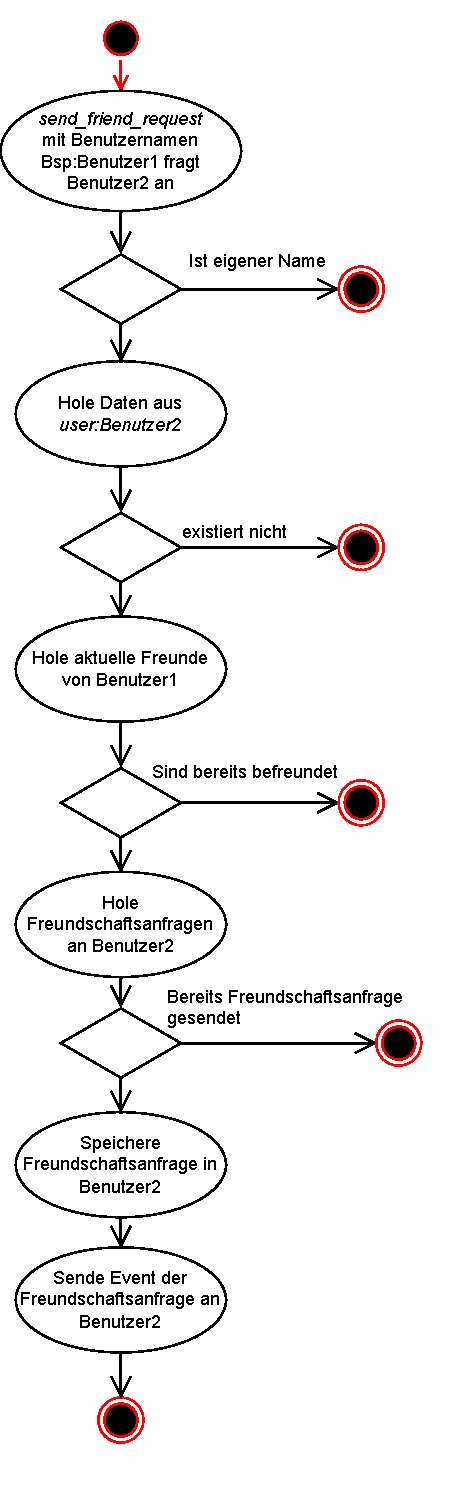
\includegraphics[width=\linewidth]{Freunde-adden.pdf}
  \caption{Senden einer Freundschaftsanfrage}
  \label{fig:friend_request}
  \end{subfigure}
  \hspace{10mm}
  \begin{subfigure}[b]{0.3\textwidth}
  \centering
    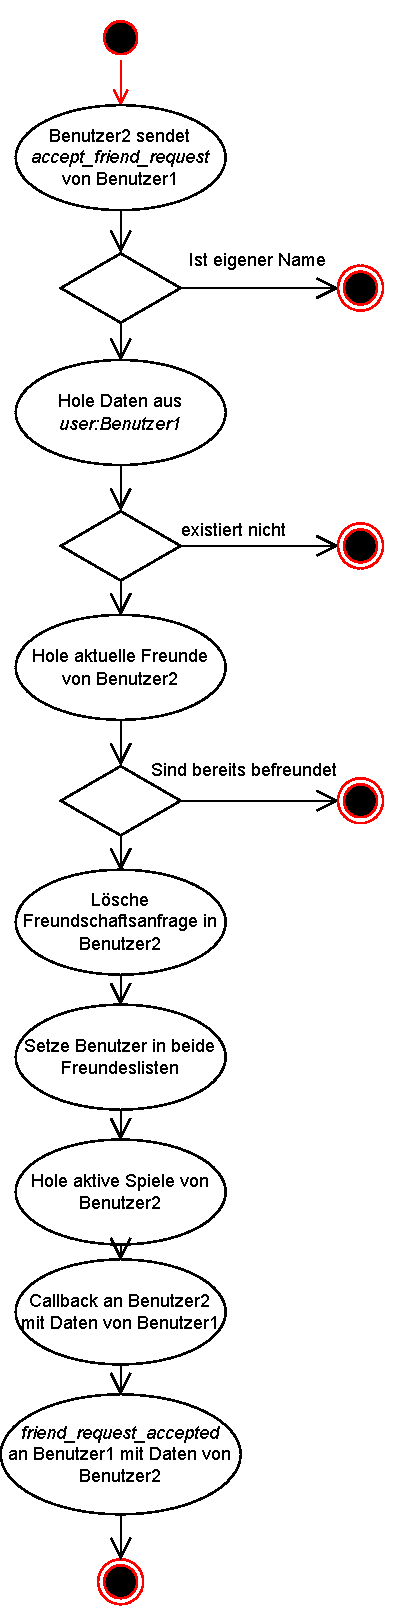
\includegraphics[width=\linewidth]{Freund akzeptieren.pdf}
  \caption{Akzeptieren einer Freundschaftsanfrage}
  \label{fig:friend_request}
  \end{subfigure}
  \caption{Aktivitätsdiagramme des Versenden und Akzeptieren von Freundschaftsanfragen}
  \label{fig:Freunde-backend}
 
\end{figure}

		\section{Datenbankstruktur}
\subsection{PostgreSQL Datenbank}
Die PostgreSQL Datenbank wird ausschließlich für die Anmeldung und Registrierung genutzt. Sie enthält eine Tabelle mit folgendem Schema:
\begin{itemize}
\item \textbf{id:} Eine Fortlaufende id, die als Primärschlüssel dient.
\item \textbf{email:} Die E-Mail, die bei der Registrierung angegeben wurde.
\item \textbf{username:} Der Benutzername des Benutzers.
\item \textbf{userid:} Jeder Spieler erhält beim Registrieren seine eigene userid. Diese dient der Kommunikation mit dem Benutzer. Bei einer Verbindung mit Socket.io erhält die socket immer eine andere ID, also wie sendet man ein Event an einen bestimmten Spieler? Diese \verb|userid| löst das Problem, indem man nach dem anmelden immer dieser ID als Raum beitritt (siehe Kapitel \ref{sec:socketauth}). Somit kann immer an diese ID gesendet werden und man stellt sicher, dass der Client das Event empfängt.
\item \textbf{password:} Das mit bcrypt verschlüsselte Passwort des Benutzers.
\end{itemize}
Jedes dieser Attribute, außer das Passwort, hat die Einschränkung, dass es einzigartig sein muss. Die E-Mail wird bisher nicht genutzt, kann aber in Zukunft zum Bestätigen der Registrierung oder Einrichtung eines Newsletters genutzt werden.

\subsection{Redis}
\label{sec:redis-data}

Bemerkung: Bei beispielsweise \verb|user:username| oder \verb|username:userid| wird der \verb|username| immer mit dem richtigen Benutzernamen ausgetauscht. Also die konkreten Zuweisung wäre somit beispielsweise \verb|user:Max| oder \verb|Max:18b06...|
\subsubsection{user:username}
Unter dem Key \verb|user:username| befindet sich ein Redis Hash. Ein Redis Hash besitzt Key-Value Paare, auf welche man zugreifen kann.

In unserem Fall werden folgende Values zu den Keys dort gespeichert:
\begin{itemize}
\item \textbf{userid:} Auch hier wird die userid gespeichert, da Redis vor allem für socket.io Funktionen verwendet wird und daher eine kurze Abfragezeit benötigt.
\item \textbf{connected:} Ist \glqq true\grqq{ }oder \glqq false\grqq , je nachdem ob der Benutzer gerade online ist oder nicht.
\item \textbf{activeGames:} Eine Liste in der alle roomIds der aktuellen Spiele des Benutzers gespeichert sind
\end{itemize}

\subsubsection{game:roomId}
\label{sec:game:roomId}
Der Redis Hash \verb|game:roomId| verwaltet die Daten einer Schachpartie. Dazu gehören:
\begin{itemize}
\item \textbf{whitePlayer, blackPlayer:} Benutzernamen des weißen und schwarzen Spielers.
\item \textbf{time:} Der Zeitmodus welcher gespielt wird (z.B.: 15 + 10, 5 + 3, ...)
\item \textbf{pgn:} Die Historie aller bisherigen Züge im PGN Format.
\item \textbf{chat:} Alle bisher geschriebenen Nachrichten im Chat.
\end{itemize}

\subsubsection{friends:username}
\label{sec:friends:username}
Der Key \verb|friends:username| verweist auf eine Liste von Freunden. Diese Freunde bestehen aus einem String, der sich zusammensetzt aus \verb|username:userid|. Dies verhindert, dass wenn ein Event an einen Freund gesendet werden soll, man einen extra Zugriff auf \verb|user:username| machen muss um die \verb|userid| zu bekommen.

\subsubsection{friend\_requests:username}
Dies ist eine Liste die genauso aufgebaut ist wie die \verb|friends:username| Liste, außer, dass sie Freundschaftsanfragen verwaltet.

\subsubsection{Warteschlangen}
\label{sec:Warteschlange}
Die Warteschlangen für Partien mit zufälligem Gegner bestehen aus \linebreak \verb|waitingPlayers:timeMode| und \verb|waitingGuests:timeMode|, je nachdem, ob es sich um einen angemeldeten Benutzer handelt oder nicht. \verb|timeMode| repräsentiert hier alle möglichen Schachuhren, also beispielsweise \glqq 10 + 5\grqq , \glqq 15 + 10\grqq , ...

Diese Warteschlagen sind Listen, welche aus \verb|username:userid| Einträgen bestehen, um zu verhindern, dass ein weiterer Zugriff auf \verb|user:username| nötig ist, um die \verb|userid| zu bekommen. 

Durch die Redis Operationen \verb|RPOP| und \verb|LPUSH| lassen sich atomar Einträge hinzufügen oder herausnehmen, welches die Konsistenz der Liste gewährleistet.

\section{Testen der Anwendung}
Während der Entwicklung der Schach-App, wurden die Funktionen ausgiebig getestet, um die Richtigkeit der Implementierung zu gewährleisten. Aufgrund der begrenzten Zeit wurde der Schwerpunkt auf das Testen des Zusammenspiels zwischen Frontend und Backend gelegt, statt auf ausgiebige Tests der einzelnen Codeausschnitte des Front- und Backends.

Um die Funktionsweise der verschiedenen Komponenten zu überwachen wurden viele Konsolenausgaben genutzt, um zu überprüfen, dass die Anwendung das gewünschte Verhalten aufzeigt und um Fehlerquellen zu identifizieren.

Es ist zu beachten, dass dieser Ansatz zwar eine schnelle und effektive Methode zum Testen der Hauptfunktionalitäten darstellt, jedoch möglicherweise nicht alle möglichen Fehlerfälle oder Randbedingungen abdeckt. Für die zukünftige Entwicklung wäre es sinnvoll, den Testprozess zu strukturieren und ausgiebige Tests für das Front- und Backend durchzuführen, um die Stabilität der Anwendung zu verbessern.
\newpage
\newpage\thispagestyle{empty}\hspace{1em}\newpage

\chapter{Implementierung}
Grobe Funktionsweisen der Implementierung wurden bereits im Kapitel Systemarchitektur erläutert. In diesem Kapitel wird auf detaillierte Implementierungsaspekte anspruchsvoller Prozesse mit Hilfe von Codeausschnitten eingegangen. Funktionen, die weniger komplex sind und deren Behandlung im Kapitel Systemarchitektur als ausreichend angesehen wird, werden nicht erneut thematisiert.
    \section{Frontend-Entwicklung}
    \subsection{Authentifizierung}
    \label{sec:Auth-Impl-Front}
Die verschiedenen Art und Weisen und Abläufe der Authentifizierung wurde im Kapitel \ref{sec:Autehtifizierung Frontend} behandelt.
In diesem Kapitel werde ich näher auf die genaue Implementierung dieser Abläufe eingehen, erklären wie die Formik Formulare funktionieren und konkrete Codeausschnitte vorstellen.
    \subsubsection{Erster Versuch der Authetifizierung mittels Cookie}
    \label{sec:Cookie-auth}
Im Codeausschnitt \ref{lst:AccountContext} ist der Code der gesamten AccountContext Datei zu sehen, welche den \textit{UserContext} zur Verfügung stellt.

\begin{lstlisting}[style=codeStyle, caption={Die AccountContext.js-Datei}, label={lst:AccountContext}]
import React, {useEffect, useState, createContext} from "react";

export const AccountContext = createContext();

const UserContext = ({children}) => {
    const [user, setUser] = useState({loggedIn: null});

    useEffect(() => {
        fetch(`${process.env.REACT_APP_API_URL}/auth/login`, {
            credentials: "include",
        })
            .catch(err => {
                console.log(err);
                return;
            })
            .then(r => {
                if (!r || !r.ok || r.status >= 400) {
                    return;
                }
                return r.json();
            })
            .then(data => {
                setUser({ ...data});
            });
    }, []);
    return (
        <AccountContext.Provider value ={{user, setUser}}>
            {children}
        </AccountContext.Provider>
    );
}
export default UserContext;
\end{lstlisting}


In ihr wird der State \verb|user| mit \verb|{loggedIn: null}| initialisiert. Weshalb wir dies tun wird durch den Codeausschnitt \ref{lst:Views-user-socket} und dessen Erklärung in Abschnitt \ref{sec:socket-Verbindung} ersichtlich. Sobald die Komponente gerendert wurde, wird die Funktion der \verb|useEffect|-Hook ausgeführt. Das leere Dependency Array verursacht, dass sie nur beim starten der Anwendung ausgeführt wird. Die Funktion schickt eine HTTP GET-Anfrage unter \verb|/auth/login| an den Server mit der Option, dass Credentials mitgesendet werden sollen. Dies stellt sicher, dass der Cookie mit dem JWT-Token an den Server gesendet wird und dort verifiziert werden kann\footnote{Quelle: \url{https://javascript.info/fetch-crossorigin} am 11. Mai 2023}. Der restliche Pfad ist als Umgebungsvariable gesetzt um den Pfad flexibel ändern zu können.

Gibt es einen Fehler oder eine ungültige Antwort wird der Vorgang abgebrochen, ansonsten wird der \verb|user| mit den erhaltenen Daten gesetzt.

Mögliche Optionen sind dabei:
\begin{itemize}
\item \verb|{loggedIn: false}|, falls man nicht authentifiziert werden konnte.
\item \verb|{loggedIn: true, username: Max}|, bei erfolgreichem Authentifizieren. (Max ist hier nur ein Beispiel als username)
\end{itemize}
Mehr Informationen benötigt der Benutzer aktuell nicht über sich selbst.

\subsubsection{Authentifizierung mittels \textit{SignUp}- oder \textit{Login}-Komponente}
Um sich mit Hilfe von den \textit{SignUp}- oder \textit{Login}-Komponenten anzumelden wird eine HTTP POST-Anfrage an den Server unter dem Pfad \verb|/auth/login| oder \verb|/auth/signup| gesendet.

Die Funktion zum Senden der Login-Daten an den Server befindet sich in Codeausschnitt \ref{lst:submitLogin}.

\begin{lstlisting}[style=codeStyle, caption={Die Funktion zum Senden der Benutzerdaten an das Backend}, label={lst:submitLogin}]
    const submitLogin = useCallback((values, setSubmitting) => {
        fetch(`${process.env.REACT_APP_API_URL}/auth/login`, {
            method: "POST",
            credentials: "include",
            headers: {
                "Content-Type": "application/json",
            },
            body: JSON.stringify(values)
        })
            .catch(err => {
                setLoginError("Please try again later");
                setSubmitting(false);
                return;
            })
            .then(res => {
                if (!res || !res.ok || res.status >= 400) {
                    setSubmitting(false);
                    setLoginError("Please try again later");
                    return;
                }
                return res.json();
            })
            .then(data => {
                if (!data.loggedIn) {
                    setLoginError(data.message);
                    setSubmitting(false);
                    return;
                }
                setUser({...data});
                setLoginError(null);
                navigate('/');
            });
    }, [setLoginError, setUser, navigate]);
\end{lstlisting}

Die Funktion zum Senden der Registrierungs-Daten ist ähnlich aufgebaut, nur dass die Anfrage an einen anderen Pfad geht und es mehr Daten enthält, wie zum Beispiel die E-Mail.

Initialisiert wird die Funktion mittels der \textit{useCallback}-Hook um unnötige Neuerstellungen zu vermeiden (siehe Kapitel \ref{sec:react}). Der \glqq Content-Type\grqq{ }hilft dem Server zu erkennen um was für eine Art von Daten es sich handelt\footnote{Quelle: \url{https://javascript.info/fetch} am 11. Mai 2023}, während im Body die angegebenen Anmeldedaten als String verpackt werden. Falls der Server mit einem Fehler Antwortet, wird dieser durch den State \verb|loginError| erfasst und dargestellt. Ansonsten wird der Benutzerstatus gesetzt und es wird auf den Pfad \verb|/| navigiert, auf der sich die \textit{Home}-Komponente befindet.

Das Formular wird mittels Formik reaktiv und nutzt Yup Schemata zum Überprüfen der eingegebenen Werte.

\begin{lstlisting}[style=codeStyle, caption={Ein Ausschnitt der \textit{Login}-Komponente mit Formik}, label={lst:Login_Formik}]
...
<Formik
    initialValues={{
        username: "",
        password: "",
    }}
    validationSchema={LoginSchema}
    validateOnChange={true}
    onSubmit={(values, { setSubmitting }) => {
        submitLogin(values, setSubmitting);
    }}
>
    {({ isValid, isSubmitting }) => (
        <Form style={{ width: "100%" }}>
        		...
            <Field name="password">
               {({ field, form }) => (
                  <FormControl isInvalid={form.errors.password && form.touched.password}>
                      <FormLabel htmlFor="password">Password</FormLabel>
                      <InputGroup>
                           <Input {...field} 
                           	id="password" 
                           	type={showPassword ? 'text' : 'password'} 
                           	autoComplete="current-password" />
                           <InputRightElement>
                               <IconButton
                                   icon={showPassword ? <ViewOffIcon /> : <ViewIcon />}
                                   onClick={handlePasswordClick}
                                   variant="ghost"
                                   _hover={{ bg: hover }}
                                   aria-label="Toggle password visibility"
                               />
                           </InputRightElement>
                       </InputGroup>
                       <FormErrorMessage>{form.errors.password}
                       </FormErrorMessage>
                   </FormControl>
               )}
            </Field>
            ...
            <Button
                type="submit"
                isDisabled={!isValid || isSubmitting}
                ...
            >
               Log In
            </Button>
            ...
\end{lstlisting}

In diesem Codeausschnitt ist das von Formik verwaltete Formular der \textit{Login}-Komponente zu erkennen (die Komponente ist in Abbildung \ref{fig:Login} dargestellt). Als Schema für dieses Formular wird das Yup Schema \verb|LoginSchema| verwendet (siehe Codeausschnitt \ref{lst:Yup-Login}) und es wird definiert, dass bei jeder neuen Änderung der Eingabefelder des Formulars, die Eingaben auf das Schema getestet werden sollen (siehe Zeilen 7 \& 8 des Codeausschnitts \ref{lst:Login_Formik}).

\verb|isValid| und \verb|isSubmitting| (siehe Zeile 13 des Codeausschnitts \ref{lst:Login_Formik}) sind props, die man von Formik zur Verfügung gestellt bekommt und die angeben, ob die Eingabefelder mit dem Schema übereinstimmen und ob gerade noch auf die Antwort des Servers gewartet wird. Dies ist auch der Grund, warum wir \verb|setSubmitting| der \verb|submitLogin| Funktion übergeben (siehe Zeile 9 des Codeausschnitts \ref{lst:Login_Formik}). Wird noch auf die Antwort des Servers gewartet oder das Formular stimmt nicht mit dem Schema überein, wird der Button deaktiviert, sodass man ihn nicht mehr klicken kann zum Absenden (siehe Zeile 42 \& 43 des Codeausschnitts \ref{lst:Login_Formik}).

Als Eingabefelder, gibt es  den Benutzernamen und das Passwort. Aus Demonstrationszwecken habe ich in den Codeausschnitt \ref{lst:Login_Formik} nur das Passwort eingefügt.

Die Props \verb|field| und \verb|form| (siehe Zeile 17 des Codeausschnitts \ref{lst:Login_Formik}) versorgen das Feld mit Informationen und Funktionen für das Feld und über das gesamte Formular. So wird in Zeile 21 das Input Feld mit dem \verb|field| prop verknüpft, welches Attribute wie die Funktion \verb|field.onChange| oder \verb|field.value| besitzt. \verb|form| wird genutzt um Beispielsweise wie in Zeile 35 ein Fehler beim Passwort anzuzeigen, falls dies nicht mit dem Schema übereinstimmt\footnote{Quelle: \url{https://formik.org/docs/api/field} am 11. Mai 2023}.

Gestaltet wird das Formular mit Komponenten von Chakra UI, welche viele hilfreiche Komponenten wie \verb|FormErrorMessage| oder \verb|IconButton| bereitstellt. Mit Attributen wie \verb|_hover| oder \verb|variant| können diese Komponenten noch weiter individualisiert werden (siehe Kapitel \ref{sec:Design}).

Die \textit{Login}-Komponente besitzt den boolean State \verb|showPassword|, welcher angibt, ob das Passwort zu sehen sein soll oder nicht (siehe Zeile 23 des Code Ausschnitts \ref{lst:Login_Formik}). Bei einem Klick auf das Icon mit dem Auge wird die Funktion \verb|handlePasswordClick| ausgeführt, welche den \verb|showPassword| State negiert. Je nach dem aktuellen Wert des States \verb|showPassword| wird ein Auge oder ein durchgestrichenes Auge als Icon angezeigt.

Die Formulierung von Schemata mittels Yup ist relativ simpel.

\begin{lstlisting}[style=codeStyle, caption={Yup Schma für das Anmelden}, label={lst:Yup-Login}]
const LoginSchema = Yup.object().shape({
    username: Yup.string()
        .min(3, 'Username has to be at least 3 characters long')
        .max(20, 'Username cannot be longer than 20 characters')
        .test('not_guest', 'Username cannot start with "guest"', (value) => {
            return !value.startsWith('guest');
        })
        .test('no colon', 'Username cannot include ":"', (value) => {
            return !value.includes(':');
        })
        .required('Username is a required field'),
    password: Yup.string()
        .min(8, 'Password has to be at least 8 characters long')
        .minLowercase(1, 'At least one character hat to be in lower case')
        .minUppercase(1, 'At least one character has to be in upper case')
        .minNumbers(1, 'At least on character has to be a number')
        .minSymbols(1, 'At least one character has to be a symbol')
        .minRepeating(3, 'It is only allowed to have at most 3 repeating characters')
        .required('Password is a required field'),
});
\end{lstlisting}

In diesem Beispiel ist das \verb|LoginSchema| zu sehen, welches für die Validierung der Eingabefelder im Anmeldeformular aus Codeausschnitt \ref{lst:Login_Formik} verwendet wird. Yup ermöglicht es bestimmte Restriktionen an Eingabefelder zu stellen und dabei direkt die Fehlernachrichten zu definieren, falls eine Restriktion nicht erfüllt ist. Selbstverständlich sind die Restriktionen für das Registrieren die gleichen, wobei das Registrierungsformular noch ein paar weitere Felder hat.

Verwendet werden übliche Restriktionen an Benutzernamen und Passwörter, sodass das Passwort mindestens eine Nummer, ein Symbol, einen Großbuchstaben, ... beinhalten muss. Eine Sonderheit ist, dass der Benutzername nicht mit \glqq guest\grqq{ }beginnen darf (siehe Zeile 5 f. des Codeausschnitts \ref{lst:Yup-Login}), da unangemeldete Benutzer bei Schachpartien einen solchen Benutzernamen zugewiesen bekommen (siehe Kapitel \ref{sec:Schach-Backend-impl}). Eine zweite Sonderheit ist, dass der Benutzername keinen Doppelpunkt beinhalten darf. Dies liegt daran, dass wir in der Redis Datenbank öfters die \verb|userid| mit dem Benutzernamen mit einem Doppelpunkt in einem String verbinden (siehe Kapitel \ref{sec:friends:username}).


\subsubsection{Socket.io Verbindungsaufbau}
\label{sec:socket-Verbindung}
Immer sobald sich der Benutzerzustand ändert wird eine Socket.io Verbindung hergestellt und den anderen Komponenten zur Verfügung gestellt. Dies hat den Nutzen, dass beim Verbindungsaufbau immer auch die socket auf dem Server authentifiziert werden muss.

Dafür wird die \textit{SocketContext}-Komponente verwendet:

\begin{lstlisting}[style=codeStyle, caption={Die Datei \textit{SocketContext.js}}, label={lst:SocketContext}]
import {io} from "socket.io-client";
import React, {useContext, useEffect, useState, createContext} from "react";
import {AccountContext} from "./AccountContext.js";

export const SocketContext = createContext();

function SocketConnectionContext({children}) {
    const [socket, setSocket] = useState(null);
    const {user} = useContext(AccountContext);

    useEffect(() => {
        if(user.loggedIn !== null) {
            if(socket) {
                socket.disconnect();
            }
            setSocket(new io(process.env.REACT_APP_SOCKET_URL, {
                withCredentials: true
            }));
        }
    }, [user]);

    return (
        <SocketContext.Provider value={{socket}}>
            {children}
        </SocketContext.Provider>
    );
}

export default SocketConnectionContext;
\end{lstlisting}

Bei der Verbindung wird darauf geachtet, dass die Credentials mitgesendet werden, also beispielsweise auch Cookies. Des weiteren wird erst eine Verbindung aufgebaut, sobald die Antwort des Servers auf die Authentifizierungs-Anfrage mittels Cookie (siehe Abschnitt \ref{sec:Cookie-auth}) empfangen wurde und dadurch das \verb|user.loggedIn| Attribut nicht mehr \verb|null| ist. Dies dient dazu einen unnötigen Verbindungsaufbau zu unterlassen, da nach der Antwort des Servers in der \textit{UserContext}-Komponente ohnehin eine neue Verbindung aufgebaut werden würde.
Die Verbindung der Socket zu trennen vor der neuen Verbindung hat den Sinn, im Backend ein \verb|diconnect| Event zu triggern (siehe Kapitel \ref{sec:Backend-Socket}).

Erst sobald die erste Authentifizierung stattgefunden hat und eine Socket.io Verbindung hergestellt wurde, werden die verschiedenen Elemente und Routen in der \verb|Views|-Komponente definiert. So lange wird ein Lade-Bildschirm gezeigt (siehe Codeausschnitt \ref{lst:Views-user-socket}).

\begin{lstlisting}[style=codeStyle, caption={Ausschnitt der \textit{Views}-Komponente}, label={lst:Views-user-socket}]
		   ...
        {user.loggedIn === null || socket === null ?
                <Flex align="center" justify="center" direction="column" height="80vh">
                    <Heading as='h2' size='lg'>Loading...</Heading>
                    <Spinner size='xl' color="purple.500" marginTop="4"/>
                </Flex>

                :
                <>
                    <Navbar/>
                    ...
\end{lstlisting}

\subsection{Das Schachspiel}
In diesem Abschnitt werde ich darauf eingehen, was passiert nachdem die Daten erfolgreich vom Backend empfangen wurden, wie ein neuer Zug gehandhabt wird und wie die Bauernumwandlung implementiert ist.
Der Ablauf wie ein Gegner gefunden wird, wie auf die \textit{ChessGame}-Komponente navigiert wird und welche Daten von dem Backend empfangen werden befindet sich in Kapitel \ref{sec:Schachspiel}.

\subsubsection{Initialisierung nach dem Empfangen der Daten}


\begin{lstlisting}[style=codeStyle, caption={Initialisierung des Schachspiels nach Empfangen der Daten}, label={lst:chessground}]
useEffect(() => {
    if(initialized) {
            setGround(new Chessground(document.getElementById(roomId), {
                fen: chess.fen(),
                orientation: orientation,
                viewOnly: isSpectator,
                movable: {
                    free: false,
                    color: orientation,
                    showdests: true
                },
                premovable: {
                    enabled: false
                },
                animation: {
                    enabled: true,
                    duration: 400
                }
            }));
    }
}, [initialized]);
    
useEffect(() => {
    if(ground) {
        ground.set({
            movable: {
                events: {
                    after: onMove(ground, chess)
                }
            }
        });
        refreshBoard(ground, chess);        
        socket.on('opponent_move', (move) => {
            if(move.flags.includes('p')) {
                onOpponentPromotion(move);
                return;
            }
            ground.move(move.from, move.to);
            chess.move(move);
            if(move.flags.includes('e')) {
                onEnPassent(ground, move);
            }
            refreshBoard(ground, chess);
        });
        socket.on('cancel_game', () => {...});
        socket.on('time_over', (color) => {...});
        socket.on('checkmate', (winner) => {...});
        socket.on('draw', () => {...});
        socket.on('resigned', (color) => {...});
    }
    return () => {
        socket.off('opponent_move');
        socket.off('Checkmate');
        socket.off('draw');
        socket.off('time_over');
        socket.off('cancel_game');
        socket.off('resigned');
    }
}, [socket, ground, initialized, ground, chess, orientation, whitePlayer, blackPlayer]);
\end{lstlisting}

Sobald erfolgreich die Daten mit dem \verb|get_game_data| Event empfangen und gesetzt wurden, wird \verb|initialized| auf true gesetzt, um die nächsten Schritte in Gang zu leiten.

Zunächst wird ein chessground Objekt mit Konfigurationen erstellt. In diesem wird übermittelt, wie die Figuren gerade stehen (mittels FEN-Notation), die Orientierung welche Farbe nach unten zeigen soll, ob man Figuren bewegen darf und wenn ja welche und weitere Optionen. Dieses chessground Interface wird dann in dem definierten div Bock angezeigt (siehe Zeile 3 des Codeausschnitts \ref{lst:chessground}).

Wurde dann chessground initialisiert, wird noch die Methode \verb|onMove| zu chessground hinzugefügt, die ausgeführt werden soll, wenn man selbst einen Zug macht (siehe Zeile 28 Codeausschnitt \ref{lst:chessground}) und Listener für verschiedene Events des Schachspiels werden initialisiert. Diese Listener werden wieder entfernt (siehe Zeile 52 ff. in Codeausschnitt \ref{lst:chessground}), falls die \textit{ChessGame}-Komponente verlassen wird, da sie nur für dieses Spiel auf die Events hören sollen und bei einem neuen Spiel neue Listener initialisiert werden.

Nach jedem Zug, egal ob eigener oder eines Gegners, wird die \verb|refreshBoard| Methode aufgerufen.

\begin{lstlisting}[style=codeStyle, caption={Die refreshBoard Methode}, label={lst:refreshBoard}]
export function refreshBoard(ground, chess) {
    ground.set({
        turnColor: toColor(chess),
        movable: {
            dests: getValidMoves(chess)
        }
    });
}
\end{lstlisting}

Diese Methode sorgt dafür, dass eine Figur von chessground nur auf legale Züge ziehen darf und korrekt aktualisiert wird, welcher Spieler an der Reihe ist.

Ein \verb|move| Objekt, das zurückgegeben wird nach dem ziehen eines Zuges auf einem chess.js Objekt (siehe \verb|move| Parameter Zeile 35 in Codeausschnitt \ref{lst:chessground} oder Zeile 10 Codeausschnitt \ref{lst:onMove})) ist folgendermaßen aufgebaut\footnote{Quelle: \url{https://github.com/jhlywa/chess.js/} am 08. Mai 2023}:
\begin{verbatim}
{ color: 'w', from: 'e2', to: 'e4', flags: 'b', piece: 'p', san: 'e4' }
\end{verbatim}
Vor allem relevant sind die flags dieses Objekts, da sie ausdrücken um was für eine Art von Zug es sich handelt. Wird als flag beispielsweise \glqq e\grqq{ }angegeben, handelt es sich um ein En passent. Bei einem \glqq p\grqq{ }liegt eine Bauernumwandlung vor.
Je nachdem ob eines dieser flags vorhanden ist, wird der Zug anders verarbeitet. Wie ein gegnerischer Zug behandelt wird (siehe Zeile 33 ff. in Codeausschnitt \ref{lst:chessground}), ist in Kapitel \ref{sec:Das-Schachspiel-Front} erläutert.

\subsubsection{Neuer Zug}

\begin{lstlisting}[style=codeStyle, caption={Die onMove Methode}, label={lst:onMove}]
const onMove = useCallback(() => {
    return (orig, dest) => {
    		//Promotion
        if((dest.includes('8') || dest.includes('1')) && chess.get(orig).type === 'p') { 
            setSelectVisible(true);
            setPromotionMove([orig, dest]);
            return;
        }
        const player = (orientation === 'white') ? whitePlayer : blackPlayer;
        const move = chess.move({from: orig, to: dest});
        socket.emit('new_move',roomId, player, move, ({done, errMsg}) => {
            if(!done) {
                chess.undo();
                ground.set({fen: chess.fen()});
                toast({
                    title: "Invalid Move",
                    description: errMsg,
                    status: "error",
                    position: "top",
                    isClosable: true
                });
                refreshBoard(ground, chess);
                return;
            }
        });
        if(move.flags.includes('e')) {
            onEnPassent(ground, move);
        }
        refreshBoard(ground, chess);
    };
}, [socket, chess, roomId, ground, orientation, setSelectVisible, setPromotionMove, whitePlayer, blackPlayer]);
\end{lstlisting}

Die \verb|onMove| Methode, welche ausgeführt wird, sobald auf dem chessground Interface eine Figur von dem Spieler bewegt wurde, behandelt, wie schon in Abschnitt \ref{sec:Das-Schachspiel-Front} erläutert, en passant- und Bauernumwandlungszüge gesondert. Wenn es sich um eine Bauernumwandlung handelt (ein Zug in Reihe 1 oder 8 mit einem Bauern), wird \verb|selectVisible| auf true gesetzt, welches bewirkt, dass die Komponente \textit{PromotionModal} sein Modal öffnet und man eine Figur auswählen kann, in welche der Bauer transformiert werden soll. Um die Felder dieses Zuges zu speichern und außerhalb dieser Methode Verfügbar zu machen, werden sie in den State \verb|promotionMove| gespeichert (siehe Zeile 6 des Codeausschnitts \ref{lst:onMove}).

\begin{lstlisting}[style=codeStyle, caption={Die promotion Methode}, label={lst:promotion}]
const promotion = useCallback(
    (toPiece) => {
        const move = chess.move({from: promotionMove[0], to: promotionMove[1], promotion: toPiece});
        ground.state.pieces.set(promotionMove[1], {
            role: charPieceToString(toPiece),
            color: parseInt(promotionMove[1].split('')[1]) === 8 ? 'white' : 'black',
            promoted: true
        });
        const player = (orientation === 'white') ? whitePlayer : blackPlayer;
        socket.emit('new_move', roomId, player,  move, ({done, errMsg}) => {
            if(!done) {
                chess.undo();
                ground.set({fen: chess.fen()});
                toast({
                    title: "Invalid Move",
                    description: errMsg,
                    status: "error",
                    position: "top",
                    isClosable: true
                });
                refreshBoard(ground, chess);
                return;
            }
        });
        setPromotionMove([]);
        setSelectVisible(false);
        refreshBoard(ground, chess);
    },
    [socket, roomId, chess, ground, promotionMove]
);
\end{lstlisting}

Wurde auf eine Figur des Modals geklickt, wird von dort die Methode \verb|promotion| mit der entsprechenden Figur ausgeführt. Dann wird sowohl auf der chess.js, als auch auf der chessGround Instanz diese Bauernumwandlung durchgeführt, an das Backend gesendet und die States \verb|promotionMove| und \verb|selectVisible| werden zurückgesetzt. Da chess.js und chessground verschiedene Notationen der Figuren verwenden transformiert die Funktion \verb|charPieceToString| die Notation der Figuren beispielsweise von \glqq q\grqq{ } in \glqq queen\grqq . Die Farbe der Figur wird durch die Reihe ermittelt in der die Bauernumwandlung stattfindet (siehe Zeile 6 des Codeausschnitts \ref{lst:promotion}).

\subsubsection{Schachuhr}
\label{sec:impl-schachuhr}
Die Komponente \textit{ChessClock} übernimmt die Verwaltung und die Darstellung der Schachuhren. Die Listener dieser Komponente wurden in Kapitel \ref{sec:Frontend-Uhr} erläutert.

\begin{lstlisting}[style=codeStyle, caption={Ausschnitt der \textit{ChessClock}-Komponente}, label={lst:ChessClock}]
...
const currentTimer = useRef(0);
...
socket.on('updated_time', (timeWhite, timeBlack, turn) => {
            stopClocks();
            updateTime(timeWhite, timeBlack);
            setCurrentTurn(turn);
        });
...
useEffect(() => {
    if(currentTurn === 'off') {
        return;
    }
    const functionMap = {
        tw: setTimeWhite,
        tb: setTimeBlack,
        sw: setStartingTimeWhite,
        sb: setStartingTimeBlack,
    };
    const setFunction = functionMap[currentTurn];
    const id = setInterval(() => {
        decrease(setFunction);
    }, 1000);
    currentTimer.current = id;
    return () => {
        clearInterval(id);
    }
}, [currentTurn]);
\end{lstlisting}

Mit diesem Beispiel kann man gut demonstrieren, wie vielfältig die \verb|useEffect|-Hook genutzt werden kann. Man nutzt in diesem Fall keine selbst definierte Funktion um eine Zeit zu starten, sondern nutzt die Eigenschaft der Hook, dass sie ausgeführt wird sobald sich ein Wert des Dependecy Arrays (in diesem Fall \verb|currentTurn|) ändert, um eine Zeit starten zu lassen. Den State der Zeit die ablaufen soll wird mittels \verb|currentTurn| definiert. Diese kann die folgenden Werte annehmen:

\begin{itemize}
\item \glqq sw\grqq : Die Startzeit von Weiß läuft.
\item \glqq sb\grqq : Die Startzeit von Schwarz läuft
\item \glqq tw\grqq : Die reguläre Zeit von Weiß läuft.
\item \glqq tb\grqq : Die reguläre Zeit von Schwarz läuft.
\item \glqq off\grqq : Keine Zeit läuft.
\end{itemize}

Diese Werte werden auch in der serverseitigen Schachuhr verwendet (siehe Kapitel \ref{sec:Uhr-Backend-impl}).

Die \verb|setInterval|-Methode (siehe Zeile 21 ff. des Codeausschnitte \ref{lst:ChessClock}) akzeptiert als ersten Parameter eine Funktion und als zweiten Parameter eine Zahl, die das Zeitintervall in Millisekunden angibt, in dem die Funktion ausgeführt werden soll. In unserem Fall soll die verbleibende Zeit jede Sekunde um eine Sekunde reduziert werden. Die \verb|setInterval|-Methode gibt eine ID zurück, die in der \verb|useRef|-Variable \verb|currentTimer| gespeichert wird. Im Vergleich zur \verb|useState|-Hook hat die \verb|useRef|-Hook den Vorteil, dass sie keine Neurenderung der Komponente auslöst, wenn sich der Wert ändert, und besser geeignet ist, um Werte über mehrere Rendervorgänge hinweg persistent zu speichern\footnote{Quelle: \url{https://react.dev/reference/react/useRef} am 09. Mai 2023}.

Über \verb|currentTimer| kann in anderen Funktionen, beispielsweise beim Anhalten einer Uhr, auf die ID zugegriffen werden, und die \verb|setInterval|-Funktion kann mit \\ \verb|clearInterval(currentTimer.current)| gestoppt werden.

\subsection{Verwaltung von Freunden}
Die Verwalutung von Freunden und Freundschaftsanfragen im Frontend wurde in Kapitel \ref{sec:Friends} behandelt. In diesem Kapitel möchte ich konkrete Code Beispiele der Komponenten erläutern.

\subsubsection{Darstellung der Freundesliste}
\begin{lstlisting}[style=codeStyle, caption={Darstellung der Freundesliste in \textit{FriendList}}, label={lst:FriendList}]
{friends.length === 0 ? (
    <Text>No Friends</Text>
  ) : (
    <>
      {friends
        .slice()
        .sort((a, b) => (a.connected === "true") - (b.connected === "true"))
        .map((friend) => (
          <Friend key={friend.username} friend={friend} times={props.times} />
        ))}
    </>
  )
}
\end{lstlisting}

Die Darstellung von Daten in Arrays kann in React mittels der Array \verb|map()| Funktion unkompliziert gehandhabt werden. Doch vor der Darstellung wird die Freundesliste noch nach dem \verb|connected| Status sortiert, sodass Freunde die online sind zuerst angezeigt werden.

Dafür wird die Methode \verb|sort()| verwendet. Diese nimmt eine Funktion mit zwei Parametern (hier \verb|a| und \verb|b|) entgegen, die jeweils ein Element des Arrays sind. Gibt uns die Funktion eine positive Zahl zurück, muss Element \verb|a| vor Element \verb|b| sortiert sein. Bei negativen anders herum und bei 0 ist es gleichgültig. Indem die Booleschen Werte von einander subtrahiert werden, werden ihnen Zahlen zugeordnet: 1 für \verb|true| und 0 für \verb|false|. Nun haben wir die folgenden Szenarien: Wenn beide den gleichen Status haben ist der Wert 0. Ist \verb|a.connected| true und \verb|b.connected| ist false: 1-0=1 $\Rightarrow$ \verb|a| wird vor \verb|b| sortiert. Anders herum dem entsprechend 0-1=-1.

Die Darstellung und Funktionen eines einzelnen Freundes übernimmt die \textit{Friend}- Komponente, die ihre Daten als props übergeben bekommt.

Auch die Liste der Freundschaftsanfragen, die Liste der aktiven Spiele der \textit{ActiveGames}- oder \textit{Friend}-Komponente wird mittels der \verb|map()| Funktion durch einzelne Komponenten dargestellt.

\subsubsection{connected-Event}
\label{sec:connected}
Eine andere Interessante Methode der \textit{FriendList}-Komponente ist der Listener auf das \verb|connected| Event:

\begin{lstlisting}[style=codeStyle, caption={Der connected Eventlistener der \textit{FriendList}-Komponente}, label={lst:routing-Middlewares}]
socket.on('connected', (status, username) => {
    setFriends(prevFriends => {
        return [...prevFriends].map(friend => {
            if (friend.username === username) {
                friend.connected = status;
            }
            return friend;
        });
    });
});
\end{lstlisting}

Dieses Event wird ausgelöst, wenn ein Freund die Anwendung öffnet oder schließt beziehungsweise sich anmeldet oder abmeldet. Dabei wird die Freundesliste mit der Funktion \verb|map()| durchlaufen und der Status des entsprechenden Freundes wird aktualisiert. Der Code zum Senden dieses Events vom Backend wird in Kapitel \ref{sec:Backend-Socket} dargestellt.


\subsubsection{Nutzung von refreshKey}
\begin{lstlisting}[style=codeStyle, caption={Darstellung der Freundesliste in \textit{FriendList}}, label={lst:FriendList}]
//Home.js
...
const [refreshKey, setRefreshKey] = useState(0);
const refreshData = useCallback(() => {
    setRefreshKey((prevKey) => prevKey + 1);
}, [setRefreshKey, refreshKey]);

useEffect(() => {
    refreshData();
}, [location.pathname]);
...
//FriendList
useEffect(() => {
    socket.emit('get_friends', ({friendList}) => {
        setFriends(friendList);
    });
    socket.emit('get_friend_requests', ({requests}) => {
        setFriendRequests(requests);
    });
}, [socket, props.refreshKey]);
\end{lstlisting}

\verb|refreshKey| ist ein State, welcher den Komponenten \textit{FriendList} und \textit{ActiveGames} übergeben wird. Dieser State ist dient dazu die Freundesliste, Freundschaftsanfragen und aktive Partien aus dem Backend zu holen und zu aktualisieren. Wird beispielsweise von der \textit{ChessGame}-Komponente auf die \textit{Home}-Komponente navigiert, werden die Komponenten neu gerendert, doch die \verb|useEffect|-Hooks werden nur neu ausgeführt, wenn eines der Elemente im Dependency Array geändert wurde. Um sicherzustellen, dass die Daten ordnungsgemäß aktualisiert werden wird der \verb|refreshKey| dem Dependency Array hinzugefügt.


\subsection{Design}
\label{sec:Design}
In diesem Abschnitt geht es um Code-Beispiele des Frontend Designs mittels Chakra UI.  Wie schon in der Zielsetzung \ref{sec:Zielsetzung} besprochen ist das Design bisher nicht responsiv.

Chakra UI stellt Komponenten zum Gestalten zur Verfügung, so ist zum Beispiel die Komponente \verb|<Box>| vergleichbar mit einer \verb|<div>| Komponente und \verb|<Text>| mit \verb|<p>|. Diesen Komponenten lassen sich Attribute geben, um die Anpassbarkeit der Elemente zu erhöhen.

\begin{lstlisting}[style=codeStyle, caption={Darstellung der \textit{Friendlist} und \textit{ActiveGames} Komponenten in der \textit{Home}-Komponente}, label={lst:impl-Home}]
...
const backgroundBox = useColorModeValue("white", "purple.500");
...
{user.loggedIn === true ?
<Box backgroundColor={backgroundBox} borderRadius="md" marginLeft={3} p={6}
     boxShadow="0 4px 6px -1px rgba(0, 0, 0, 0.1), 0 2px 4px -1px rgba(0, 0, 0, 0.06)">
    <Text marginBottom={1} fontSize="1.2rem"> Active Games: </Text>
    <ActiveGames refreshKey={refreshKey}/>
    <Text marginTop={5} fontSize="1.2rem"> Friends: </Text>
    <FriendList refreshKey={refreshKey} times={times}/>
</Box>
:
<>
</>
}
\end{lstlisting}

In diesem Codeausschnitt der \textit{Home}-Komponente wird die \textit{FriendList} und \textit{ActiveGames} gerendert siehe Abbildung \ref{fig:home-logged-in}).

Verwendet wird der Ternäre Operator, um die Komponenten nur anzuzeigen, falls der Benutzer angemeldet ist (siehe Zeile 4 des Codeausschnitts \ref{lst:implHome}). Ist er nicht angemeldet wird das React Fragment \verb|<> </>| gerendert. Ein React Fragment ermöglicht die Gruppierung von Komponenten ohne einen \verb|<div>| Block verwenden zu müssen, da das React Fragment nicht in der DOM gerendert wird\footnote{Quelle: \url{https://react.dev/reference/react/Fragment} am 11. Mai 2023}.  In diesem Fall dient das React Fragment dazu, nichts zu rendern, falls der Benutzer nicht angemeldet ist.

Die Chakra UI Syntax für die Attribute einer Komponente erinnert an die CSS Syntax. So steht das Attribut \verb|p={6}| für das Padding \footnote{Quelle: \url{https://chakra-ui.com/docs/styled-system/style-props} am 11. Mai 2023}. Es handelt sich dabei allerdings nicht um sechs Pixel, sondern Chakra UI verwendet seine eigene Größenzuordnung. In diesem Fall entspricht das 1.5rem.

Um die Anwendung sowohl in einem dunklen Modus, als auch einem hellen Modus anzupassen, gibt es die Funktion \verb|useColorModeValue|\footnote{Quelle: \url{https://chakra-ui.com/docs/styled-system/color-mode} am 11. Mai 2023}. Diese Funktion lässt uns Werte je nach Modus definieren. In unserem Beispiel hat die \verb|<Box>|-Komponente die Hintergrundfarbe Weiß im hellen Farbschema und Lila im dunklen Farbschema.

\begin{lstlisting}[style=codeStyle, caption={Verwendung von einem Thema mit Chakra UI}, label={lst:themes.js}]
//App.js
...
<ChakraBaseProvider theme={customTheme}>
    ...
</ChakraBaseProvider>
...

//themes.js
const customTheme = extendTheme({
    overrides,
    fonts: {
        heading: `'Exo 2', sans-serif`,
        body: `'Exo 2', sans-serif`,
    },
    components: {
        Button: {
            variants: {
                'start-game-light': {
                    bg: "gray.200",
                    color: "black",
                    _hover: {
                        bg: "purple.200",
                    }
                },
                'start-game-dark': {
                    bg: "purple.700",
                    color: "white",
                    _hover: {
                        bg: "purple.600"
                    }
                },
                ...
//Home.js
...
const startGameButton = useColorModeValue("start-game-light", "start-game-dark");
...
<Button variant={startGameButton} ... > {time.string} </Button>
...
\end{lstlisting}

Chakra UI ermöglicht die Verwendung eines Themas, auf die man in allen Unterkomponenten der \textit{ChakraBaseProvider}-Komponente (siehe Abschnitt \ref{sec:React-Komponenten}) zugreifen kann\footnote{Quelle: \url{https://chakra-ui.com/docs/styled-system/customize-theme} am 11. Mai 2023}. In dem Beispielcode sieht man die Definition von zwei verschiedenen Buttons, die die Optik der Knöpfe in der \textit{Home}-Komponente zum Starten eines Spiels definieren. Diese Optik wird in einigen anderen Komponenten wiederverwendet, weshalb sie in der \verb|themes.js| Datei definiert werden, um eine bessere Wartbarkeit, Anpassbarkeit und Wiederverwendbarkeit zu gewährleisten.


    \section{Backend-Entwicklung}
    \subsection{Authentifizierung}
    \label{sec:Backend-auth-impl}
Die Vorgehensweise im Backend bei der Authentifizierung des Benutzers ist im Kapitel \ref{sec:Authentifizierung Backend} geschildert. In diesem Kapitel werde ich Code Beispiele vorstellen und erläutern.

\subsubsection{Routing-Middlewares}
Der Codeausschnitt \ref{lst:routing-Middlewares} zeigt die Reihenfolge der Middlewares bei den Anmelde- und Registrierungsanfragen des Frontends.
\begin{lstlisting}[style=codeStyle, caption={Ausschnitt aus index.js und die Datei authRouter.js}, label={lst:routing-Middlewares}]
//index.js
...
app.use("/auth", authRouter);
...

//authRouter.js
const express = require('express');
const router = express.Router();
... //import der Middlewares

router.use(rateLimiter(60, 10));

router.route('/login').get(handleLogin).post(validateLogin, attemptLogin);

router.post('/signup', validateSignUp, attemptSignUp);

router.get('/logout', handleLogout);

module.exports = router;
\end{lstlisting}

Für jede Anfrage auf den Pfad \verb|/auth| wird die Middleware \verb|rateLimiter| verwendet (siehe Zeile 11 des Codeausschnitts \ref{lst:routing-Middlewares}). Dieser achtet darauf, dass nicht zu viele Anfragen einer IP Adresse gesendet werden. 

\begin{lstlisting}[style=codeStyle, caption={Die rateLimiter Middleware}, label={lst:rateLimiter}]
const redisClient = require("../redis/redis.js");

module.exports.rateLimiter = (secondsLimit, limitAmount) => async (req, res, next) => {
    const ip = req.connection.remoteAddress;
    [response] = await redisClient
        .multi()
        .incr(ip)
        .expire(ip, secondsLimit)
        .exec();
    if (response[1] > limitAmount) {
        res.json({
            loggedIn: false,
            message: "Slow down!! Try again in a minute.",
        });
    }
    else next();
};
\end{lstlisting}

Der \verb|rateLimiter| nimmt die Argumente secondsLimit als Zeitfenster und limitAmount als Anfragelimit an und definiert mit Hilfe von ihnen die Middleware. Dafür nutzt er Redis und setzt mit der IP-Adresse als Key die Zahl der Anfragen als Value\footnote{Quelle: \url{https://redis.io/commands/incr/} am 11. Mai 2023}. Dieser Eintrag wird nach Ablauf des Zeitfensters gelöscht und falls das Anfragelimit innerhalb dieses Zeitfensters überschritten wurde, wird eine Fehlermeldung gesendet. Andernfalls wird die nächste Middleware aufgerufen.

In unserer Anwendung legen wir fest, dass 10 Anfragen innerhalb von 60 Sekunden gesendet werden dürfen.

Für die erste Authentifizierung im \textit{UserContext} (siehe Abschnitt \ref{sec:Cookie-auth}) wird die Middleware \verb|handleLogin| verwendet (siehe Zeile 13 des Codeausschnitts \ref{lst:routing-Middlewares}).

\begin{lstlisting}[style=codeStyle, caption={Die handleLogin Middleware zum Authentifizieren mit Cookie}, label={lst:handleLogin}]
const getJwtFromCookie = req => {
    return req.headers["cookie"] && cookie.parse(req.headers["cookie"])["jwt"];
};

module.exports.handleLogin = (req, res) => {
    const token = getJwtFromCookie(req);
    if(!token) {
        res.json({loggedIn: false});
    } else {
        jwt.verify(token, process.env.JWT_SECRET, (err, decodedPayload) => {
            if (err) {
                res.json({loggedIn: false});
            } else {
                res.json({loggedIn: true, username: decodedPayload.username});
            }
        });
    }
};
\end{lstlisting}

Diese Middleware ließt gegebenenfalls den Cookie mit dem JWT-Token und antwortet entsprechend ob er ihn erfolgreich dekodieren konnte oder nicht.

Bei den POST Anfragen des Frontends, über die das ausgefüllte Anmelde-, beziehungsweise Registrierungsformular gesendet wird, wird vor der Auswertung mit den Middlewares \verb|validateLogin| oder \verb|validateSignUp| überprüft, ob das Formular auch dem entsprechenden Yup Schema übereinstimmt. Anschließend wird mit \verb|attemptLogin| oder \verb|attemptSignUp| versucht den Benutzern anzumelden oder zu registrieren.

\begin{lstlisting}[style=codeStyle, caption={Die attemptLogin Middleware zum Anmelden}, label={lst:attemptLogin}]
module.exports.attemptLogin = async (req, res) => {
    const potentialLogin = await query(
        "SELECT id, username, password, userid FROM users u WHERE u.username=$1",
        [req.body.username]
    );
    if (potentialLogin.rowCount > 0) {
        const isSamePassword = await bcrypt.compare(
            req.body.password,
            potentialLogin.rows[0].password
        );
        if (isSamePassword) {
            const user = {
                username: req.body.username,
                userid: potentialLogin.rows[0].userid,
            }
            jwt.sign(
                user,
                process.env.JWT_SECRET,
                {expiresIn: "24h"},
                (err,token) => {
                if(err) {
                    res.json({loggedIn: false, message: "Something went wrong, try again later"});
                } else {
                    const jwtCookie = cookie.serialize("jwt", token, {
                        httpOnly: true,
                        secure: process.env.NODE_ENV === "production", // Secure flag only in production
                        maxAge: 24 * 60 * 60, // 24 hours
                        sameSite: "lax",
                        path: "/"
                    });
                    res.setHeader("Set-Cookie", jwtCookie);
                    res.json({loggedIn: true,  username: user.username});
                }
            }
            );
        } else {
            res.json({loggedIn: false, message: "Wrong username or password!"});
        }
    } else {
        res.json({loggedIn: false, message: "Wrong username or password!"});
    }
};
\end{lstlisting}

Die Middleware \verb|attemptLogin| überprüft zunächst, ob ein Benutzer mit diesem Benutzernamen in der PostgreSQL-Datenbank existiert und mittels bcrypt ob die Passwörter übereinstimmen. Dafür wird die \verb|query|-Funktion (siehe Kapitel \ref{sec:Datenbank-Integration}) genutzt, indem in der Tabelle \verb|users| nach einem Eintrag mit dem Benutzernamen gesucht wird. Der SQL-String verwendet den Platzhalter \verb|$1|, der durch den Wert \verb|[req.body.username]| ersetzt wird\footnote{Quelle: \url{https://node-postgres.com/features/queries} am 11. Mai 2023}. Existiert kein Benutzer mit diesem Benutzernamen oder ist das Passwort falsch wird das Frontend darüber benachrichtigt. Ansonsten wird ein 24 Stunden haltbarer JWT-Token mit dem Benutzernamen und der \verb|userid| generiert und in einen Cookie mit dem Key \glqq jwt\grqq{ }gesetzt, welcher ebenfalls 24 Stunden gültig ist. Der JWT-Token beinhaltet die \verb|userid|, da die Socket Verbindung diese Information beim authentifizieren benötigt (siehe Abschnitt \ref{sec:Backend-Socket}).  Wichtig dabei ist, dass das Attribut \verb|httpOnly| auf \verb|true| gesetzt wird, um zu verhindern, dass Client seitiger Code auf den Cookie zugreifen könnte. Anschließend wird dem Frontend noch mit dem JSON Objekt geantwortet (siehe Zeile 39).

Beim Registrieren wird ebenfalls bei Erfolg der Cookie mit dem JWT-Token gesetzt, jedoch sind die Anforderungen natürlich andere. Es wird überprüft, ob bereits ein Account mit dem Benutzernamen oder der E-Mail existiert und falls ja wird dem Frontend entsprechend geantwortet. Ansonsten wird eine zufällige \verb|userid| erstellt, das Passwort mit bcrypt verschlüsselt, der Tupel in der Datenbank gespeichert und der Cookie mit dem JWT-Token gesetzt.

\subsubsection{Abmelden}
Da das Abmelden auch gewissermaßen zum Authentifizierungsprozess gehört, wird hier kurz beschrieben, was im Backend dabei passiert.

\begin{lstlisting}[style=codeStyle, caption={Middleware zum Abmelden}, label={lst:handleLogout}]
module.exports.handleLogout = (req, res) => {
    res.setHeader(
        "Set-Cookie",
        cookie.serialize("jwt", "", {
            httpOnly: true,
            secure: process.env.NODE_ENV === "production",
            maxAge: -1,
            sameSite: "lax",
            path: "/"
        })
    );
    res.sendStatus(204);
}
\end{lstlisting}

Eine Anfrage zum Abmelden wird auf den Pfad \verb|auth/logout| gestellt unter der die Middleware aus Codeausschnitt \ref{lst:handleLogout} durchlaufen wird. In dieser wird ein leerer (siehe Zeile 4), abgelaufener(siehe Zeile 7) \glqq jwt\grqq -Cookie gesetzt, der bewirkt, dass der bisherige \glqq jwt\grqq -Cookie gelöscht wird. Dann wird dem Frontend mit dem Code 204 geantwortet (siehe Zeile 12), welcher aussagt, dass die Anfrage erfolgreich bearbeitet wurde, jedoch keine Daten mit der Antwort gesendet werden\footnote{Quelle \url{https://developer.mozilla.org/en-US/docs/Web/HTTP/Status/204} am 05. Mai 2023}.

\subsubsection{Socket.io Authentifizierung und Middleware}
\label{sec:Backend-Socket}
Im Codeausschnitt \ref{lst:index.js-socket} ist ein Ausschnitt der index.js Datei zu sehen, in der der Socket.io Server initialisiert wird und die Middlewares für socket Verbindungen zugewiesen werden.

\begin{lstlisting}[style=codeStyle, caption={Ausschnitt der index.js Datei mit Socket.io Server Erstellung und Middleware Zuweisung}, label={lst:index.js-socket}]
...
const corsConfig = {
    origin: process.env.FRONTEND_URL,
    credentials: true,
}
const server = require('http').createServer(app);
const io = new Server(server, {
    cors: corsConfig
});
io.use(authorizeUser);
io.use(initializeUser);
io.use((socket, next) => {
    initializeChessListeners(socket, io);
    initializeListeners(socket, io);
    next();
});
...
\end{lstlisting}

Die Initilaisierung des Socket.io Servers benötigt die \verb|corsConfig| Konfiguration, um Verbindungen vom Frontend zuzulassen und Header Informationen wie Cookies mitzusenden.

Es werden drei Middlewares bei einem Verbindungsaufbau durchlaufen,  die ich in diesem Kapitel mit Codeausschnitten erläutern werde.


\begin{lstlisting}[style=codeStyle, caption={authorizeUser Middleware für Socket.io Verbinudngen}, label={lst:authorizeUser}]
module.exports.authorizeUser = (socket, next) => {
    let token = null;
    if (socket.request.headers.cookie) {
        token = cookie.parse(socket.request.headers.cookie).jwt;
        if (token) {
            jwt.verify(token, process.env.JWT_SECRET, (err, decodedPayload) => {
                if (err) {
                    next(new Error('Unable to Read Token'));
                    return;
                }
                socket.user = {...decodedPayload};
            });
        }
    }
    next();
}
\end{lstlisting}

Die Middleware \verb|authorizeUser| (siehe Codeausschnitt \ref{lst:authorizeUser}) authentifiziert den Benutzer. Dabei  wird auf den Cookie zugegriffen, der gegebenenfalls gesetzt wurde, um den Benutzernamen und die \verb|userid| als Attribute der socket zu setzen (siehe Zeile 11 des Codeausschnitts \ref{lst:authorizeUser}). Diese Middleware ist der Grund, warum immer eine neue Socket.io Verbindung hergestellt werden muss, sobald der Benutzerzustand und damit der Cookie sich verändert. Ansonsten könnte es sein, dass veraltete Informationen in \verb|socket.user| definiert sind.

\begin{lstlisting}[style=codeStyle, caption={initializeUser Middleware für Socket.io Verbinudngen}, label={lst:initializeUser}]
module.exports.initializeUser = async (socket, next) => {
    if (socket.user) {
        socket.join(socket.user.userid);
        await setUser(socket.user.username, socket.user.userid, true);
        getFriends(socket.user.username).then(async friends => {
            const friendRooms = friends.map(friend => friend.userid);
            if (friendRooms.length > 0) {
                socket.to(friendRooms).emit("connected", "true", socket.user.username);
            }
        });
    }
    next();
};
\end{lstlisting}

In der Middleware \verb|initializeUser| wird der Nutzer als online vermerkt, seine Freunde werden darüber informiert, dass er nun online ist und er tritt dem Raum seiner \verb|userid| bei. Dies passiert natürlich nur, wenn in der vorherigen Middleware der Benutzer authentifiziert werden konnte. Die Funktion \verb|setUser| setzt den Eintrag \verb|user:username| mit der \verb|userid| und \verb|connected| auf true. Die Methode \verb|getFriends| (siehe Kapitel \ref{ref:getFriends}) holt die Benutzernamen und die \verb|userid|s aller Freunde des Benutzers und mittels der map Funktion wird an alle \verb|userid|s der Freunde das Event \verb|connected| gesendet. Dadurch wird im Frontend der Spieler als online angezeigt (siehe Abschnitt \ref{sec:connected}). 

Die dritte Middleware setzt alle nötigen Listener für Events, die mit dem Schachspiel zusammenhängen, als auch sonstige Funktionen (siehe Zeilen 12 ff. des Codeausschnitts \ref{lst:index.js-socket}).

\begin{lstlisting}[style=codeStyle, caption={Die onDisconnect Methode für Sockets}, label={lst:onDisconnect}]
module.exports.onDisconnect = async (socket) => {
    if (!socket.user) {
        return;
    }
    await setUser(socket.user.username, socket.user.userid, false);
    getFriends(socket.user.username).then(friends => {
        const friendRooms = friends.map(friend => friend.userid);
        if (friendRooms.length > 0) {
            socket.to(friendRooms).emit("connected", "false", socket.user.username);
        }
    });
}
\end{lstlisting}

Die \verb|onDisconnect| Methode aus Codeausschnitt \ref{lst:onDisconnect} wird aufgerufen, sobald eine socket Verbindung getrennt wird. Hierfür dient der \verb|socket.disconnect()| Aufruf des Frontends (siehe Abschnitt \ref{sec:socket-Verbindung}). Ähnlich wie bei der \verb|initializeUser| Middleware (siehe Codeausschnitt \ref{lst:initializeUser}) wird dabei in Redis der Spieler als offline vermerkt und seine Freunde werden mit dem Event \verb|connected| darüber in Kenntnis gesetzt.


\subsection{Das Schachspiel}
\label{sec:Schach-Backend-impl}
Das Schachspiel verwaltet die Datei \verb|socketChessController.js|, welche eine der Funktionen zur Listener Initialisierung bereitstellt (siehe \verb|initilializeChessListeners| aus Codeausschnitt \ref{lst:index.js-socket}), wobei \verb|ServerChessClock.js| die Schachuhren bereitstellt.

In diesem Abschnitt werde ich einige Aspekte der Implementierung des Schachspiels mit Code Beispielen erläutern. Funktionen wie Aufgeben, das Ende der Partie oder Chat Nachrichten werden im Abschnitt \ref{sec:Schach-Backend} erläutert und zeichnen sich durch geringere Komplexität aus, weshalb sie in diesem Abschnitt nicht nochmals behandelt werden. Auch das Finden eines Gegners wird in dem Abschnitt der Backend-Architektur detailliert beschrieben, weshalb dies hier nicht noch einmal erläutert wird.

\subsubsection{Initialisierung eines Spiels}
\label{sec:init-backend}
Die Suche und das Finden eines Gegners wurde in Abschnitt \ref{sec:find_game} erläutert. In diesem Abschnitt möchte ich genauer darauf eingehen, wie ein Spiel nach gefundenem Gegner initialisiert wird. Dabei handelt es sich um die \verb|createChessGame| Methode (für Kontext siehe Sequenzdiagramm in Abbildung \ref{fig:sequence_chess_start}).

\begin{lstlisting}[style=codeStyle, caption={Die createChessGame Methode zum Initialisieren einer Schachpartie}, label={lst:createChessGame}]
const createChessGame = async (io, username1, username2, time) => {
    const roomId = UUIDv4();
    const [whitePlayer, blackPlayer] = Math.random() < 0.5 ? [username1, username2] : [username2, username1];

    const chessInstance = await import('../chess/Chess.mjs').then(ChessFile => {
        return ChessFile.Chess();
    });
    const d = new Date();
    chessInstance.header('White', whitePlayer, 'Black', blackPlayer, 'Date', d.toDateString());
    //Store Game in Redis
    await initializeGame(roomId, whitePlayer, blackPlayer, time, chessInstance.pgn());
    const chessClock = new ServerChessClock(time);
    currentChessClocks[roomId] = {chessClock};

    chessClock.startStartingTimer('white');
    chessClock.ChessClockEvents.on('cancel_game', () => {
        io.to(roomId).emit('cancel_game');
        io.to(roomId).emit('stop_clocks');
        endGame(roomId)
    });
    chessClock.ChessClockEvents.on('time_over', (color) => {
        io.to(roomId).emit('time_over', color);
        io.to(roomId).emit('stop_clocks');
        endGame(roomId);
    });
    return roomId;
}
\end{lstlisting}

Die \verb|createChessGame| Methode legt zunächst per Zufall fest, welcher Spieler welche Farbe spielen soll und generiert eine zufällige ID als roomId in der das Spiel stattfindet. Anschließend wird ein chess.js Objekt erstellt. Da es sich bei der Bibliothek chess.js um ein ECMAScript-Module handelt und node.js ein CommonJS-Modulsystem verwendet muss man einen Umweg mittels einer \verb|.mjs|-Datei zum Importieren der Bibliothek verwenden\footnote{Quelle: \url{https://stackoverflow.com/questions/70396400/how-to-use-es6-modules-in-commonjs} am 06. Mai 2023} (siehe Codeausschnitt \ref{lst:Chess.mjs}).

\begin{lstlisting}[style=codeStyle, caption={Die Chess.mjs Datei}, label={lst:Chess.mjs}]
import {Chess as ChessGame} from 'chess.js';
export const Chess = () => new ChessGame();
\end{lstlisting}

Mit diesem chess.js Objekt generieren wir eine PGN-Notation, in die die Benutzernamen der Spieler und das Datum eingetragen sind. Diese Informationen werden mittels der \verb|initializizeGame| Methode in Redis unter \verb|game:roomId| gespeichert. Falls die Spieler angemeldet sind wird die roomId auch in die Listen \verb|activeGames| der \verb|user:username| Einträge der beiden Spieler hinzugefügt. 

Des weiteren wird ein ServerChessClock Objekt erstellt und in \verb|currentChessClock| mit der roomId als Key gespeichert. Die Kommunikation und der Aufbau von ServerChessClock wird in Abschnitt \ref{sec:Uhr-Backend-impl} erläutert.
Eventlistener für die Events \verb|time_over| und \verb|cancel_game| der ServerChessClock werden definiert. \verb|cancel_game| ist ein Event, welches ausgelöst wird, falls eine Startzeit abgelaufen ist und \verb|time_over|, falls eine reguläre Zeit abgelaufen ist.
Da die Schachuhren und das Schachspiel möglichst Modular gehalten werden, wird an das Frontend in diesen Listenern immer zwei Events gesendet: \verb|time_over|, beziehungsweise \verb|cancel_game| für das Schachspiel und \verb|stop_clocks| für die Schachuhren im Frontend. Bei jeder Möglichkeit wie eine Schachpartie endet wird definiert, dass die Funktion \verb|endGame| ausgeführt werden soll, so auch bei diesen zwei Listenern. Was bei diese Methode bewirkt wird in Kapitel \ref{sec:Schach-Ende} erläutert.

\subsubsection{Neue Züge}
\label{sec:new_move_backend}
Beim Eingang eines neuen Zugs mittels des \verb|new_move| Events wird die Methode \verb|newMove| ausgeführt. Sie benötigt die socket des Spielers und die Socket.io Server Instanz. Die restlichen Daten die sie benötigt werden vom Frontend mit dem Event mitgesendet.

Ein Aktivitätsdiagramm und eine ausführliche Erklärung des Ablaufs wird in Abschnitt \ref{sec:Zug-Backend} behandelt. In diesem Abschnitt konzentrieren wir uns auf die Umsetzung dieser Aktivitäten im Code.
\begin{lstlisting}[style=codeStyle, caption={newMove Methode die beim Eingang eines neuen Zugs aufgerufen wird}, label={lst:newMove}]
//Listener:
client.on('new_move', newMove(client, io));
//Methode
const newMove = (socket, io) => async (roomId, player, move, cb) => {
    if(!currentChessClocks[roomId]) {
        cb({done: false, errMsg: "Game does not exist"});
        return;
    }
    const {chessClock} = currentChessClocks[roomId];
    const chessInstance = await import('../chess/Chess.mjs').then(ChessFile => {
        return ChessFile.Chess();
    });
    try {
        chessInstance.loadPgn(await getGame(roomId, "pgn").then(pgn => {
            if(!pgn) {
                cb({done: false, errMsg: "Game does not exist"});
                return;
            }
            return pgn;
        }));
        chessInstance.move(move)
    } catch(error) {
        cb({done: false, errMsg: error});
        return;
    }
	
    socket.to(roomId).emit('opponent_move', move);
    //Store move in Redis
    newChessMove(chessInstance.pgn(), roomId).then(r => cb({done: true}));
    
    if(chessInstance.isGameOver()) {
        if (chessInstance.isCheckmate()) {
            io.to(roomId).emit('checkmate', socket.user.username);
        } else {
            io.to(roomId).emit('draw');
        }
        io.to(roomId).emit('stop_clocks');
        chessClock.ChessClockEvents.emit('stop');
        endGame(roomId);
        cb({done: true});
        return;
    }
    
    chessClock.ChessClockEvents.emit('toggle', ({remainingTimeWhite, remainingTimeBlack, turn}) => {
        io.to(roomId).emit('updated_time', remainingTimeWhite, remainingTimeBlack, turn);
    });

    if (chessInstance.history().length === 1) {
        chessClock.startStartingTimer('black');
        io.to(roomId).emit('stop_starting_time_white');
    } else if (chessInstance.history().length === 2) {
        chessClock.startTimer('white');
        io.to(roomId).emit('stop_starting_time_black');
    }
}
\end{lstlisting}

Die Methode holt erst das ServerChessClock Objekt aus dem \verb|currentChessClocks| Array und importiert die aktuelle PGN-Notation des Schachspiels aus der Redis Datenbank in ein chess.js Objekt und macht den Zug darauf (siehe Zeilen 5 - 25 des Codeausschnitts \ref{lst:newMove}).

Die Kommunikation mit dem Frontend erfolgt über verschiedene Events wie \linebreak \verb|opponent_move|, \verb|checkmate|, \verb|draw|, \verb|stop_clocks|, \verb|updated_time|,  \linebreak \verb|stop_starting_time_white| und \verb|stop_starting_time_black|. Diese Events behandeln entweder ein Ereignis der Schachpartie oder verwalten die Schachuhren. Über die Callback Funktion wird mitgeteilt, ob der Zug erfolgreich behandelt werden konnte oder nicht.

Mit dem ServerChessClock Objekt wird mittels der Events \verb|stop| und \verb|toggle| (siehe Abschnitt \ref{sec:Uhr-Backend-impl}) und den Funktionsaufrufen \verb|startStartingTimer| und \verb|startTimer| kommuniziert. \verb|stop| wird bei einem Ende der Partie gesendet, \verb|toggle| bei jedem neuen Zug, es sei denn das Spiel ist vorbei und die Funktionsaufrufe dienen zum initialen starten der Startuhren oder der regulären Uhr.

Des weiteren wird die aktualisierte PGN-Notation des Spiels mit der Funktion \linebreak \verb|newChessMove| (siehe Zeile 28 im Codeausschnitt \ref{lst:onMove}) in Redis gespeichert.

\subsubsection{Senden des aktuellen Zustands einer Partie}
Beim Laden der \textit{ChessGame}-Komponente im Frontend wird das Event \verb|get_game_data| gesendet, um den aktuellen Zustand des Spiels zu erhalten und spielen zu können beziehungsweise zugucken zu können. 


\begin{lstlisting}[style=codeStyle, caption={Der Listener des get\_game\_data Events zum übermitteln des Schachspiels}, label={lst:get_game_data}]
client.on('get_game_data', (roomId, guestName, cb) => {
    if (!currentChessClocks[roomId]) {
        cb({done: false, errMsg: "This Game does not exist"});
        return;
    }
    const {chessClock} = currentChessClocks[roomId];
    if (!client.rooms.has(roomId)) {
        client.join(roomId);
    }
    if(guestName) {
        client.user = {username: guestName}
    }
    getGame(roomId)
        .catch(() => {
            cb({done: false, errMsg: "This Game does not exist"})
        })
        .then(game => {
                if (!game) {
                    cb({done: false, errMsg: "This Game does not exist"});
                    return;
                }
                game.currentState = chessClock.getCurrentMode();
                if (game.currentState.includes('s')) {
                    game.currentStartingTimer = chessClock.getCurrentStartingTimer();
                } else {
                    game.currentTimes = chessClock.getCurrentTimes();
                }
                cb({done: true, data: game});
            }
        )
});
\end{lstlisting}

Es gibt zwei Szenarien, in denen kein Zustand des Schachspiels gesendet werden kann: Falls kein ServerChessClock Objekt in dem \verb|currentChessClocks| Array vorhanden ist (siehe Zeile 2 des Codeausschnitts \ref{lst:get_game_data}) oder falls kein Redis Eintrag zu diesem Spiel gefunden werden konnte (siehe Zeile 15 \& 18 des Codeausschnitts \ref{lst:get_game_data}).

Essenziell bei diesem Listener ist, dass die socket gegebenenfalls der roomId beitritt, um zukünftige Events, wie neue Züge, erhalten zu können. Außerdem ist es wichtig den Benutzernamen zu setzen, falls es sich um einen Gast handelt. Denn wenn dieser die Seite neu lädt wird eine neue socket Verbindung hergestellt und der Gast-Benutzername wäre nicht mehr in der socket gespeichert. Allerdings wird auf den Benutzernamen der socket beispielsweise bei einem Schachmatt zugegriffen.

Die aktuellen Daten, wie welcher Spieler welche Farbe spielt und die aktuelle PGN-Notation des Spiels werden aus Redis mittels der Funktion \verb|getGame| aus \verb|game:roomId| geholt. Fehlen nur noch die aktuellen Zeiten. Dafür verwenden wir \verb|getCurrentMode()|, um den aktuellen Zustand der Schachuhren zu bekommen (siehe Zeile 23). Dieser besteht wie im Frontend aus \glqq tw\grqq , \glqq tb\grqq , \glqq sw\grqq{ }und \glqq sb\grqq{ }(siehe \ref{sec:impl-schachuhr}). 

Je nachdem welche Uhren gerade laufen werden entweder die Startzeiten oder die reguären Zeiten der Spieler den Redis Daten hinzugefügt und anschließend dem Frontend per Callback Funktion übermittelt.

Hier wird der Sinn hinter der Speicherung des ServerChessClock Objekts in einem Array ersichtlich. Um die aktuelle Zeit abzurufen muss auf das ServerChessClock Objekt zugegriffen werden. Eine Kritik dieser Speicherungder aktuellen Zeiten und Alternativen werden in Abschnitt \ref{sec:herausforderung-Schachuhr} erläutert.

\subsubsection{Die Uhr}
\label{sec:Uhr-Backend-impl}
Die serverseitige Schachuhr wird von Objekten der Klasse \verb|ServerChessClock| verwaltet. Diese Objekte besitzen die folgenden Attribute:

\begin{lstlisting}[style=codeStyle, caption={Konstruktor der ServerChessClock Klasse}, label={lst:const-ServerChessClock}]
function ServerChessClock(time) {
    this.timeMode = time;
    this.currentMode = 'off';
    this.remainingTimeWhite = {minutes: time.minutes, seconds: 0};
    this.remainingTimeBlack = {minutes: time.minutes, seconds: 0};
    this.ChessClockEvents = new EventEmitter();
    this.startingTimeWhite = {seconds: 0};
    this.startingTimeBlack = {seconds: 0};
    switch (time.type) {
        case 'Bullet': this.startingTimeWhite.seconds = this.startingTimeBlack.seconds = 15; break;
        case 'Blitz': this.startingTimeWhite.seconds = this.startingTimeBlack.seconds = 20; break;
        case 'Rapid': this.startingTimeWhite.seconds = this.startingTimeBlack.seconds = 30; break;
        case 'Classical': this.startingTimeWhite.seconds = this.startingTimeBlack.seconds = 45; break;
        default: this.startingTimeWhite.seconds = this.startingTimeBlack.seconds = "unknown"; break;
    }
}
\end{lstlisting}

Vorab stelle ich vor, wie ein \verb|time| (siehe Zeile 1 des Codeausschnitts \ref{lst:const-ServerChessClock}) Objekt aufgebaut ist:
\begin{verbatim}
{type: 'Rapid', minutes: 15, increment: 10, string: '15 + 10'}
\end{verbatim}
\verb|type| Klassifiziert die Schachuhr Konfigurationen zu verschiedenen Modi. Diese Klassifikationen der Schachuhren sind auf online Schach-Plattformen wie \url{lichess.org} bereits Standard. Die Gründe dafür liegen vor allem in der Erweiterbarkeit (siehe //REF). Bisher werden sie genutzt um wie in Zeilen 9 ff. des Codeausschnitts \ref{lst:const-ServerChessClock} verschieden lange Startzeiten zu initialisieren.

\verb|string| dient der Darstellung und der einfachen Identifizierung dieser Objekte.

\begin{lstlisting}[style=codeStyle, caption={Die startTimer und stopCurrentGame Methoden der ServerChessClock Klasse}, label={lst:startTimer}]
ServerChessClock.prototype.startTimer = function (color) {
    this.currentMode = color === "white" ? "tw" : "tb";
    const currentPlayerTime = color === "white" ? this.remainingTimeWhite : this.remainingTimeBlack;


    const isTimeOver = () => {
        return currentPlayerTime.minutes === 0 && currentPlayerTime.seconds === 0;
    };

    const decreaseTime = () => {
        if (currentPlayerTime.seconds === 0) {
            currentPlayerTime.minutes -= 1;
            currentPlayerTime.seconds = 59;
        } else {
            currentPlayerTime.seconds -= 1;
        }
    };

    const timer = setInterval(() => {
        decreaseTime();
        if (isTimeOver()) {
            clearInterval(timer);
            this.stopCurrentGame();

        }
    }, 1000);
    
	//If game ends, because player resigned, checkmate, ...
    this.ChessClockEvents.once("stop", () => {
        clearInterval(timer);
    });
    
    //If a player played a new move
    this.ChessClockEvents.once("toggle", (cb) => {
        clearInterval(timer);
        if (color === "white") {
            this.remainingTimeWhite = increment(
                currentPlayerTime,
                this.timeMode.increment
            );
            cb({
                remainingTimeWhite: this.remainingTimeWhite,
                remainingTimeBlack: this.remainingTimeBlack,
                turn: "tb",
            });
            this.startTimer("black");
        } else {
            this.remainingTimeBlack = increment(
                currentPlayerTime,
                this.timeMode.increment
            );
            cb({
                remainingTimeWhite: this.remainingTimeWhite,
                remainingTimeBlack: this.remainingTimeBlack,
                turn: "tw",
            });
            this.startTimer("white");
        }
    });
};

ServerChessClock.prototype.stopCurrentGame = function () {
    if (this.getCurrentMode().includes('s')) {
        this.ChessClockEvents.emit('cancel_game');
    } else if (this.getCurrentMode().includes('w')) {
        this.ChessClockEvents.emit('time_over', 'white');
    } else {
        this.ChessClockEvents.emit('time_over', 'black');
    }
}
\end{lstlisting}

Die Funktion \verb|startTimer| wird ein mal von \verb|SocketChessController| aufgerufen, falls der zweite Zug gespielt wurde (siehe Zeile 52 des Codeausschnitts \ref{lst:newMove}). Anschließend wird die Methode selbst rekursiv aufgerufen, falls ein neuer Zug gespielt wurde und das \verb|toggle| Event empfangen wurde (siehe Zeile 46 \& 57 im Codeausschnitt \ref{lst:startTimer}).

Je nachdem welche Zeit läuft, wird \verb|currentMode| aktualisiert und die entsprechende Zeit wird in \verb|currentPlayerTime| referenziert (siehe Zeilen 2 \& 3 des Codeausschnitts \ref{lst:startTimer}).

Die Zeit läuft durch den \verb|timer| ab, welcher \verb|setInterval| nutzt, um jede Sekunde mittels \verb|decreaseTime| die Zeit ablaufen zu lassen und \verb|isTimeOver| um zu überprüfen ob die Zeit abgelaufen ist (siehe Zeile 19 ff. des Codeausschnitts \ref{lst:startTimer}).

Es wird ein Listener auf das Event \verb|toggle| definiert, welcher bei einem neuen Zug das Inkrement auf die entsprechende Zeit rechnet und mittels Callback Funktion die aktuellen Zeiten durchgibt (siehe Zeilen 41 ff. und 52 ff. des Codeausschnitts \ref{lst:startTimer}), um diese in der \verb|newMove| Methode an das Frontend zu senden (siehe Kapitel \ref{sec:new_move_backend}). Dieser Listener wird mit \verb|ones(...)| definiert, wodurch er nur ein mal auf das Event hört. Dies ist wichtig, da anschließend die \verb|startTimer| Methode reukursiv aufgerufen wird und der Listener neu initialisiert wird.

Die \verb|stopCurrentGame| Methode wird aufgerufen, falls eine Zeit (Startzeit oder reguläre Zeit) abgelaufen ist und sendet entsprechende Events an SocketChessController. Wie diese Events empfangen werden ist in Codeausschnitt \ref{lst:createChessGame} enthalten.


\subsection{Verwaltung von Freunden}
\label{sec:Freunde-impl}
In diesem Kapitel zeige ich die Implementierung von dem Versenden von Freundschaftsanfragen und dem senden der Freunde an das Frontend. Die zugehörigen Redis Funktionen werden in Kapitel \ref{sec:Datenbank-Integration} eräutert.

Alle anderen Funktionen welche nicht mit dem Schachspiel und der Authentifizierung zusammenhängen werden durch die Listener in der Datei \verb|socketController.js| zur Verfügung gestellt und verwenden den \verb|redisController| für Operationen an der Redis Datenbank. Der Ablauf von Funktionen im Backend bezüglich Freunden wurde ausführlich in dem Kapitel \ref{sec:hinzufügen-von-Freunden} behandelt.

\subsubsection{Versenden einer Freundschaftsanfrage}
\label{sec:Freundschaftsanfrage-backend}
\begin{lstlisting}[style=codeStyle, caption={Der Listener des send\_friend\_request Events}, label={lst:sendFriendRequest}]
client.on('send_friend_request', (requestName, cb) => {
    if(client.user) {
        requestFriend(client.user.username, client.user.userid, requestName)
        .catch(err => {            
            cb({done: false, errorMsg: "Please try again later"});
            return;
        })
        .then(result => {
                if (result.errorMsg) {
                    cb({done: false, errorMsg: result.errorMsg});
                    return;
                }
                cb({done: true});
                client.to(result.userid).emit('friend_request', client.user.username);
            }
        );
    } else {
        cb({done: false, errorMsg: "Please try again later"});
    }
});
\end{lstlisting}

Die Funktion \verb|requestFried| der \verb|redisController| Datei überprüft, ob eine Freundschaft der beiden Spieler erlaubt wäre und gibt uns unter anderem die \verb|userid| des angefragten Spielers zurück und speichert die Freundschaftsanfrage in Redis (siehe Kapitel \ref{sec:requestFriend}). Ist die Freundschaft nicht erlaubt wird die entsprechende Fehlermeldung, warum sie nicht erlaubt ist an den Sender mittels Callback Funktion weitergeleitet. Ansonsten wird die Freundschaftsanfrage mittels des Events \verb|friend_request| an den Benutzer gesendet und der Sender wird über die Callback Funktion über den erfolgreichen Versand benachrichtigt.

\subsubsection{Das Senden der Freunde ans Frontend}
\label{sec:Senden-der-Freunde}
Beim rendern der \textit{Home}-Komponente werden Events vom Frontend gesendet, um Daten wie Freunde, Freundschaftsanfragen und aktive Spiele aus der Redis Datenbank mittels Callback Funktion zu holen. Eine davon ist das \verb|get_friends| Event.

\begin{lstlisting}[style=codeStyle, caption={Der get\_friends Listener}, label={lst:get_friends}]
    client.on('get_friends', async (cb) => {
        if(client.user) {
            const friends = await getFriends(client.user.username);
            const parsedFriends = await parseFriendList(friends);
            cb({friendList: parsedFriends});
        }
    });
\end{lstlisting}

Die \verb|get_friends| Methode liefert uns die Benutzernamen und \verb|userid|s aller Freunde (siehe Kapitel \ref{sec:getFriends}), allerdings benötigt das Frontend noch weitere Daten. Das sind die aktiven Partien des Benutzers und den Status ob er gerade online ist oder nicht. Diese Daten ergänzt die Methode \verb|parseFriendList| (siehe Kapitel \ref{sec:parseFriendList}).


\section{Datenbank Integration}
\label{sec:Datenbank-Integration}
Die Herstellung einer Verbindung zu der PostgreSQL und zu der Redis Datenbank wird jeweils in einer Datei hergestellt:

\begin{lstlisting}[style=codeStyle, caption={Initialisierung der PostgreSQL Datenbank und einer Methode für die Anfragen}, label={lst:pg-pool}]
require('dotenv').config()
const Pool = require('pg').Pool

const pool = new Pool({
    user: process.env.DATABASE_USER,
    host: process.env.DATABASE_HOST,
    database: process.env.DATABASE_NAME,
    password: process.env.DATABASE_PASSWORD,
    port: process.env.DATABASE_PORT,
})

const query = (text, params) => pool.query(text, params)
module.exports = { query }  
\end{lstlisting}

\begin{lstlisting}[style=codeStyle, caption={Initialisierung einer Redis-Datebank Verbindung}, label={lst:redisClient}]
const Redis = require('ioredis');

const redisClient = new Redis();

module.exports = redisClient;
\end{lstlisting}

Die Daten zum Herstellen einer Verbindung sind in einer \verb|.env| Datei gespeichert, um die Sicherheit und Wartbarkeit zu erhöhen, da .env Dateien standardmäßig zu Dateien zählen, welche nicht in Git aufgenommen werden.

Wie die PostgreSQL Datenbank genutzt wird ist in Kapitel \ref{sec:Backend-auth-impl} erläutert. 

\subsection{Zugriff auf Redis mit dem redisController}
Alle Operationen auf der Redis Datenbank werden von der Datei \verb|redisController| zur Verfügung gestellt (mit Ausnahme der \verb|rateLimiter| Middleware). Welche Datentypen unter welchen Keys in Redis gespeichert werden, wird in Abschnitt \ref{sec:redis-data} erläutert.
Die Datei enthält 19 Methoden, die fast alle auf die Datenbank zugreifen. In diesem Abschnitt werden exemplarisch einige wichtige Methoden vorgestellt.

\subsubsection{addPlayerInQueue}

\begin{lstlisting}[style=codeStyle, caption={Methode um einen Spieler in eine Warteschlange hinzuzufügen}, label={lst:addPlayerInQueue}]
module.exports.addPlayerInQueue = async (loggedIn, time, user) => {
    return new Promise((resolve, reject) => {
        const key = loggedIn === true ? `waitingPlayers${time}` : `waitingGuests${time}`;
            redisClient.lpush(key, `${user:username}:${user:userid}`, (err, result) => {
                if (err) {
                    reject(err);
                } else {
                    resolve(result);
                }
            });
    });
};
\end{lstlisting}

Die \verb|addPlayerInQueue| Methode hat die Funktion einen Spieler in eine Warteschlange für einen zufälligen Gegner hinzuzufügen. Je nachdem ob er angemeldet ist oder nicht wird die Warteschlange \verb|waitingPlayers| oder \verb|waitingGuests| mit der entsprechenden Zeit als Key genutzt, um \verb|username:userid| in die Warteschlange zu schreiben.

Die Funktion \verb|lpush| fügt den Spieler am Anfang der Liste ein. Herausgenommen werden Spieler mittels der Funktion \verb|rpop|, die Spieler am Ende der Liste entnehmen. So wird gewährleistet, dass der Spieler der am längsten wartet zu erst entnommen wird.

Implementiert ist die Funktion durch eine \verb|Promise|, welche es ermöglicht eine Fehlerbehandlung oder ein Ergebnis einer asynchronen Methode getrennt zu behandeln\footnote{Quelle: \url{https://developer.mozilla.org/en-US/docs/Web/JavaScript/Guide/Using_promises?retiredLocale=de} am 14. Mai 2023}, beziehungsweise in diesem Fall weiter zu geben. 


\subsubsection{getFriends}
\label{sec:getFriends}
\begin{lstlisting}[style=codeStyle, caption={Methode um Freunde eines Spielers zu erhalten}, label={lst:getFriends}]
const getFriends = async (username) => {
    const friendList = await redisClient.lrange(`friends:${username}`, 0, -1);
    return friendList.map(friend => {
        return {username: friend.split(':')[0], userid: friend.split(':')[1]};
    });
}
\end{lstlisting}

Die Methode \verb|getFriends| holt alle Freunde eines Spielers aus dem key \verb|friend:username|. Mittels der Funktion \verb|lrange| können Elemente aus einer Liste geholt werden. Der Parameter \verb|0| repräsentiert den Start, ab welchem Index die Freunde geholt werden sollen und der Parameter \verb|-1| das Ende. In diesem Fall heißt \verb|-1|, dass alle Elemente aus der Liste geholt werden sollen. Die Daten werden im letzten Schritt mittels der Array \verb|map()| Funktion noch vernünftig aufbereitet um die Nutzung der Daten zu vereinfachen.

\subsubsection{parseFriendList}
\label{sec:parseFriendList}

\begin{lstlisting}[style=codeStyle, caption={Methode um alle Informationen eines Arrays von Freunden zu bekommen}, label={lst:parseFriendList}]
const parseFriendList = async (friendList) => {
    const parsedFriendList = [];
    for (let friend of friendList) {
        const parsedFriend = await getUserData(friend.username);
        const activeGames = {};
        for (let activeGame of JSON.parse(parsedFriend.activeGames)) {
            activeGames[activeGame] = await getGame(activeGame);
        }
        parsedFriendList.push({
            username: friend.username,
            userid: friend.userid,
            connected: parsedFriend.connected,
            activeGames: activeGames
        });
    }
    return parsedFriendList;
}
\end{lstlisting}

Die Methode \verb|parseFriendList| hat die Funktion alle Daten aller Freunde einer Freundesliste zu holen. Sie dient als Erweiterung der \verb|getFriends| Methode, falls mehr Daten nötig sind, als lediglich der Benutzername und die \verb|userid|. Dies ist beispielsweise für die Anzeige im Frontend der Fall (siehe Kapitel \ref{sec:Senden-der-Freunde}).

Mit einer for-Schleife wird das Array der Freunde durchlaufen und für jeden Spieler werden folgende Daten gesammelt:

\begin{itemize}
\item Online-Status \& aktive Partien: Aus dem Redis Eintrag \verb|user:username| wird mittels der \verb|getUserData| Methode alle Werte des \verb|user:username| Eintrags des Freundes geholt. Dazu zählen der online-Status und die roomIds der aktiven Partien
\item Daten der Aktiven Partien: Anschließend wird für jede aktive Partie dieses Freundes die Daten aus \verb|game:roomId| mittels der Funktion \verb|getGameData| abgerufen. Dies ist wichtig um im Frontend anzeigen lassen zu können, welche Farbe und gegen wen der Freund spielt.

\end{itemize}

Anschließend werden diese Daten in einem Objekt gesammelt und der neuen Freundesliste hinzugefügt, welche am Ende zurückgegeben wird.

\subsubsection{requestFriend und friendIsValid}
\label{sec:requestFriend}

\begin{lstlisting}[style=codeStyle, caption={requestFriend Methode um eine Freundschaftsanfrage in redis zu speichern}, label={lst:requestFriend}]
module.exports.requestFriend = async (username, userid, requestName) => {
    const requestedFriend = await friendIsValid(username, requestName);
    if (requestedFriend.errorMsg) {
        return {errorMsg: requestedFriend.errorMsg};
    }
    const currentFriendRequests = await redisClient.lrange(`friend_requests:${requestName}`, 0, -1);
    if (currentFriendRequests.includes([requestName, requestedFriend.userid].join(':'))) {
        return {errorMsg: "You've already sent a friend request to this user"};
    }
    await redisClient.lpush(`friend_requests:${requestName}`, [username, userid].join(":"));
    return {userid: requestedFriend.userid};
}
\end{lstlisting}

Die \verb|requestFriend| Methode wird beim Versenden einer Freundschaftsanfrage aufgerufen (siehe Kapitel \ref{sec:Freundschaftsanfrage-backend}), um zu überprüfen, ob eine Freundschaftsanfrage legal wäre und diese gegebenenfalls in Redis zu speichern.

Die Methode \verb|friendIsValid| überprüft, ob eine Freundschaft zulässig ist (siehe Codeausschnitt \ref{lst:friendIsValid}). Ist sie es nicht wird die entsprechende Fehlernachricht zurückgegeben. Um sicherzustellen, dass auch die Freundschaftsanfrage wirklich gültig ist, muss zusätzlich gewährleistet werden, dass zwischen den beiden Spielern keine ausstehenden Freundschaftsanfragen existieren (siehe Zeile 7 des Codeausschnitts \ref{lst:requestFriend}).

Ist dies nicht der Fall, kann die Freundschaftsanfrage der Liste unter dem Key \linebreak \verb|friend_requests:requestName| in der Form \verb|username:userid| hinzugefügt werden und die \verb|userid| des angefragten Freundes wird zurückgegeben, um an ihn die Freundschaftsanfrage zu senden (siehe Kapitel \ref{sec:Freundschaftsanfrage-backend}).

\begin{lstlisting}[style=codeStyle, caption={friendIsValid Methode um zu überprüfen, ob eine Freundschaft legal wäre}, label={lst:friendIsValid}]
const friendIsValid = async (username, requestName) => {
    if (requestName === username) {
        return {errorMsg: "You can not add yourself as a Friend"};
    }
    const friend = await getUserData(requestName);
    if (!Object.keys(friend).length) {
        return {errorMsg: "User doesn't exist"};
    }
    const currentFriendList = await redisClient.lrange(`friends:${username}`, 0, -1);
    if (currentFriendList.includes([requestName, friend.userid].join(':'))) {
        return {errorMsg: "You are already friends with that user"};
    }
    return friend;
}
\end{lstlisting}

Bei einer legalen Freundschaft muss gewährleistet sein, dass man nicht mit sich selbst befreundet sein kann (siehe Zeile 2 des Codeausschnitts \ref{lst:friendIsValid}), dass der angefragte Benutzer existiert (siehe Ziele 5 \& 6) und, dass die beiden Benutzer nicht bereits befreundet sind.

Die Überprüfung ob der Nutzer existiert, basiert darauf, dass falls er nicht existiert \verb|friend| aus einem leeren Objekt \verb|{}| besteht, was bedeutet, dass \linebreak \verb|Object.keys(friend).length| gleich 0 ist (siehe Zeile 6). Der \verb|!|-Ausdruck konvertiert diesen Wert zunächst in den booleschen Wert \verb|false| und negiert ihn anschließend, sodass der Ausdruck \verb|true| zurückgibt.


    \newpage
\newpage\thispagestyle{empty}\hspace{1em}\newpage

\chapter{Fazit und Ausblick}
    \section{Zusammenfassung der Ergebnisse}
Diese Bachelorarbeit hatte das Ziel eine Schachanwendung als Basis für Erweiterungen zu entwerfen und zu implementieren. Das Ergebnis ist eine App mit folgenden Funktionen:
\begin{itemize}
\item Schachpartien mit unterschiedlichen Zeitkonfigurationen können sowohl gegen zufällige als auch befreundete Gegner gespielt werden.
\item Das gleichzeitige Spielen mehrerer Partien ist möglich.
\item Während einer Schachpartie ermöglicht ein integrierter Chat die Kommunikation zwischen den Gegnern.
\item Zuschauer können Partien über die URL verfolgen.
\item Die Erstellung eines Accounts und die Anmeldung sind benutzerfreundlich und sicher gestaltet.
\item Das Hinzufügen von Freunden und die Anzeige ihres Online-Status sind implementiert.
\item Eine Funktion zum einfachen Wiedereinstieg in aktive Partien erleichtert das gleichzeitige Spielen mehrerer Spiele.
\end{itemize}

All diese Funktionen bilden die Grundlage für eine Schachanwendung, die besonderen Wert auf soziale Interaktionen legt. Bei der Implementierung lag der Schwerpunkt auf Modularität, Wartbarkeit, Skalierbarkeit, Erweiterbarkeit und Echtzeitkommunikation. Dafür wurden moderne Web-Technologien für eine schnelle und benutzerfreundliche Anwendung verwendet.

    \section{Herausforderungen}
In diesem Kapitel bespreche ich Herausforderungen auf die ich gestoßen bin während der Konzeption oder Implementierung der Schachanwendung. 

\subsection{Schachuhren}
\label{sec:herausforderung-Schachuhr}
Die Konzeption der Schachuhren war eine Herausforderung, die vielen verschiedene Ansätze beinhaltete. Im Endeffekt wurde sich für eine getrennte serverseitige und clientseitige Lösung entschieden (siehe Kapitel \ref{sec:Konzept-Schachuhr}). Doch auch bei dieser Lösung gab es Gestaltungsspielraum, beispielsweise wie die Zeiten konsistent gehalten werden sollten, wie das Inkrement addiert wird oder wie die verschiedenen Zeiten (Startzeit, reguläre Zeit, von weiß, von schwarz) und Events realisiert werden sollten.

Ein Problem, welches bei der Konzeption und Realisierung nur bedingt gelöst werden konnte ist die Abfrage der Zeit im Backend, wenn die Daten des Schachspiels geholt werden.

Die Frage ist, wie kann man die Zeiten konsistent im Backend speichern kann, um zu jedem Möglichen Zeitpunkt dem Frontend mitteilen zu können welche genauen Zeiten die Spieler noch haben.

Aktuell ist so realisiert, dass das ServerChessClock Objekt bei der Intitialisierung eines Schachspiels im Backend in einem Array der socketChessController Datei gespeichert wird (siehe Kapitel \ref{sec:init-backend}) und bei einer Abfrage des Frontends, das Objekt herausgenommen wird und die Zeiten übermittelt werden.

Das Problem dieser Implementierung besteht darin, dass bei vielen aktiven Partien zahlreiche ServerChessClock-Objekte den Arbeitsspeicher des Backends belegen und bei einem Neustart oder Problem des Backends das Array neu initialisiert werden könnte, wodurch alle diese Objekte verloren gehen würden. 

Somit verringert diese Implementierung sowohl die Skalierbarkeit, als auch die Wartbarkeit des Backends.

Der Grund, warum dennoch vorerst diese Implementierung gewählt wurde, liegt in den zu diesem Zeitpunkt fehlenden Alternativen. Es wäre denkbar, die aktuellen Zeiten wie die anderen Daten des Schachspiels in Redis zu speichern. Jedoch hätte eine Speicherung der aktuellen Zeit jede Sekunde viel zu viele I/O Operationen zur folge und beispielsweise nur alle 10 Sekunden die aktuellen Zeiten zu speichern würde zu einer zu großen Diskrepanz führen, wenn das Frontend in einer ungünstigen Zeit die Daten abfragen würde und es sich um ein schnelles Spiel wie \glqq 1+0\grqq{ }handeln würde. Die Speicherung der Zeit nach jedem Zug könnte auch zu sehr großen Diskrepanzen führen, wenn lange kein Zug gemacht wurde.

Eine mögliche Alternative um die Skalierbarkeit und Wartbarkeit hinsichtlich dieser Implementierung zu erhöhen und dennoch keine großen Zeitdiskrepanzen zu haben, wäre eine Lösung, bei der man bei jedem Zug die aktuellen Zeiten der Spieler und den Zeitpunkt des Zugs in Redis speichert. Sobald eine Abfrage der Daten von dem Frontend kommt, können die aktuellen Zeiten der Spieler berechnet werden, indem die Differenz zwischen dem jetzigen Zeitpunkt und dem Zeitpunkt des alten Zugs berechnet wird und diese von der Zeit des Spielers abgezogen wird, der gerade am Zug ist. Eine serverseitige Überprüfung, ob eine Zeit abgelaufen ist, müsste in einem Intervall von jeder Sekunde ausgeführt werden. Allerdings könnte man vermeiden, dass die ServerChessClock-Objekte im Arbeitsspeicher des Backends gespeichert werden müssen.

Diese Alternative scheint eine vielversprechende Möglichkeit zur Verbesserung zu sein.

\subsection{Züge des Schachspiels}
Bei der Implementierung der Behandlung eines neues Zugs im Front- und Backend sind kleinere Herausforderungen aufgekommen.

Während des Testens der Anwendung wurde festgestellt, dass chessground die Szenarien von Bauernumwandlungen und En-passant-Schlägen nicht ausreichend unterstützt und die betreffenden Figuren manuell entfernt oder ersetzt werden müssen (siehe Kapitel \ref{sec:Das-Schachspiel-Front}). Nach etwas Feinarbeit konnten diese Szenarien problemlos behandelt werden.

Im Backend trat das Problem auf, dass die Bibliothek chess.js ein ECMAScript-Module ist und Node.js das CommonJS Modulsystem verwendet. Mithilfe eines Umwegs konnte dieses Problem allerdings gelöst werden (siehe Kapitel \ref{sec:init-backend}).

\section{Zukünftige Erweiterungen und Verbesserungen}
Neben der in \ref{sec:herausforderung-Schachuhr} beschriebenen Verbesserung der Backend Schachuhr ist die Anzahl der möglichen Erweiterungen dieser Schachanwendung nahezu unbegrenzt. Einige der wichtigsten Erweiterungen, welche als nächstes angegnagen werden könnten wären:
\begin{itemize}
\item \textbf{Responsive Design}: Die Anwendung für verschiedene Geräte zu optimieren wäre ein wichtiger Schritt Richtung Veröffentlichung.
\item \textbf{Hosting}: Durch das Bereitstellen der Anwendung auf einer Hostingplattform könnte man die Anwendung der Öffentlichkeit zugänglich machen.
\item \textbf{Analysen}: Schachpartien analysieren zu können ist wichtig um aus den Fehlern der Partie zu lernen. Es gibt einige Analyseprogramme, wobei die beste derzeit Stockfish ist\footnote{Quelle: \url{https://stockfishchess.org/} am 13. Mai 2023}.
\item \textbf{Wertungen}: In Schach gibt es eine sogenannte Elo-Wertung, welche die relative Stärke eines Spielers misst\footnote{Quelle: \url{https://www.chess.com/de/terms/elo} am 13. Mai 2023}. Typischerweise besitzt jeder Spieler jeweils eine Elo für einen Zeitmodi (Bullet, Blitz, Rapid, ...). Diese Zeitmodi sind schon implementiert, sie werden nur bisher kaum genutzt (siehe Kapitel \ref{sec:Uhr-Backend-impl}).
\item \textbf{Historie vergangener Partien}: Eine Schachpartie wird bereits mit der Historie aller Züge in PGN-Notation gespeichert, wird allerdings nach dem Ende des Spiels gelöscht. Man könnte diese Datensätze wiederverwenden, um sich vergangene Spiele nochmal anschauen zu können oder teilen zu können.
\item \textbf{Zurücknehmen von Zügen}: Das Zurücknehmen eines bereits gemachten Zugs ist eine wichtige Funktion, falls man sich verklickt haben sollte. Meist schickt der Spieler eine Anfrage der Zugzurücknahme, welcher der Gegner annehmen oder ablehnen kann.
\end{itemize}

Dies sind nur einige Beispiele der von Erweiterungen welche als nächstes Angegangen werden könnten.

Da vor allem die sozialen Interaktionen dieser Schach-App ausgeprägt sein sollen, sind weitere mögliche Erweiterungen die Gründung von Clubs, welche gegeneinander in Ligen oder Turnieren antreten können, einen Clubchat haben, in dem unter anderem Partien geteilt werden können und Rollen wie Präsident, Vize-Präsident,... verteilt werden können.
 
Um das Spielen zu Belohnen könnte man Figuren-, Bretter- oder Emotedesigns als Belohnungen einführen, welche nicht nur der Spieler selber, sondern auch der Gegner sieht. Zusätzliche Belohnungen könnte man einführen durch täglich-wechselnde und statische Herausforderungen.

Dies bietet auch eine Möglichkeit der Kommerzialisierung: Nicht durch Werbung oder freischaltbare Funktionen Einnahmen generieren, sondern durch freischaltbare Designs. Die Benutzer können sich somit keinen Vorteil durch Funktionen wie Analysen oder Tutorials erkaufen, sondern ausschließlich andere Optiken.

Die Vision dieser Anwendung ist eine Schach-App, die stärker auf soziale Interaktionen und Anreize zum Spielen setzt als \url{lichess.org} und weniger kommerzialisiert ist, indem wichtige freischaltbare Funktionen nicht ausschließlich gegen Geld angeboten werden, wie es bei \url{chess.com} der Fall ist (siehe Kapitel \ref{sec:Verwandte Arbeiten}).

Insgesamt bietet diese Bachelorarbeit eine solide Grundlage für eine Schach-App, die durch soziale Interaktionen und eine Vielzahl von Funktionen den Schachspielern ein umfassendes und ansprechendes Erlebnis bietet.
\newpage

\appendix

\nocite{*}%Auch nicht-zitierte BibTeX-Einträge werden angezeigt.
\bibliography{Bibliography}

\newpage\thispagestyle{empty}\hspace{1em}\newpage
\listoffigures

\newpage\thispagestyle{empty}\hspace{1em}\newpage
\markboth{Codeausschnitte}{Codeausschnitte}
\phantomsection
\addcontentsline{toc}{chapter}{Codeausschnitte}
\lstlistoflistings


\end{document}

